% Options for packages loaded elsewhere
\PassOptionsToPackage{unicode}{hyperref}
\PassOptionsToPackage{hyphens}{url}
%
\documentclass[
]{book}
\usepackage{amsmath,amssymb}
\usepackage{lmodern}
\usepackage{iftex}
\ifPDFTeX
  \usepackage[T1]{fontenc}
  \usepackage[utf8]{inputenc}
  \usepackage{textcomp} % provide euro and other symbols
\else % if luatex or xetex
  \usepackage{unicode-math}
  \defaultfontfeatures{Scale=MatchLowercase}
  \defaultfontfeatures[\rmfamily]{Ligatures=TeX,Scale=1}
\fi
% Use upquote if available, for straight quotes in verbatim environments
\IfFileExists{upquote.sty}{\usepackage{upquote}}{}
\IfFileExists{microtype.sty}{% use microtype if available
  \usepackage[]{microtype}
  \UseMicrotypeSet[protrusion]{basicmath} % disable protrusion for tt fonts
}{}
\makeatletter
\@ifundefined{KOMAClassName}{% if non-KOMA class
  \IfFileExists{parskip.sty}{%
    \usepackage{parskip}
  }{% else
    \setlength{\parindent}{0pt}
    \setlength{\parskip}{6pt plus 2pt minus 1pt}}
}{% if KOMA class
  \KOMAoptions{parskip=half}}
\makeatother
\usepackage{xcolor}
\usepackage{color}
\usepackage{fancyvrb}
\newcommand{\VerbBar}{|}
\newcommand{\VERB}{\Verb[commandchars=\\\{\}]}
\DefineVerbatimEnvironment{Highlighting}{Verbatim}{commandchars=\\\{\}}
% Add ',fontsize=\small' for more characters per line
\usepackage{framed}
\definecolor{shadecolor}{RGB}{248,248,248}
\newenvironment{Shaded}{\begin{snugshade}}{\end{snugshade}}
\newcommand{\AlertTok}[1]{\textcolor[rgb]{0.94,0.16,0.16}{#1}}
\newcommand{\AnnotationTok}[1]{\textcolor[rgb]{0.56,0.35,0.01}{\textbf{\textit{#1}}}}
\newcommand{\AttributeTok}[1]{\textcolor[rgb]{0.77,0.63,0.00}{#1}}
\newcommand{\BaseNTok}[1]{\textcolor[rgb]{0.00,0.00,0.81}{#1}}
\newcommand{\BuiltInTok}[1]{#1}
\newcommand{\CharTok}[1]{\textcolor[rgb]{0.31,0.60,0.02}{#1}}
\newcommand{\CommentTok}[1]{\textcolor[rgb]{0.56,0.35,0.01}{\textit{#1}}}
\newcommand{\CommentVarTok}[1]{\textcolor[rgb]{0.56,0.35,0.01}{\textbf{\textit{#1}}}}
\newcommand{\ConstantTok}[1]{\textcolor[rgb]{0.00,0.00,0.00}{#1}}
\newcommand{\ControlFlowTok}[1]{\textcolor[rgb]{0.13,0.29,0.53}{\textbf{#1}}}
\newcommand{\DataTypeTok}[1]{\textcolor[rgb]{0.13,0.29,0.53}{#1}}
\newcommand{\DecValTok}[1]{\textcolor[rgb]{0.00,0.00,0.81}{#1}}
\newcommand{\DocumentationTok}[1]{\textcolor[rgb]{0.56,0.35,0.01}{\textbf{\textit{#1}}}}
\newcommand{\ErrorTok}[1]{\textcolor[rgb]{0.64,0.00,0.00}{\textbf{#1}}}
\newcommand{\ExtensionTok}[1]{#1}
\newcommand{\FloatTok}[1]{\textcolor[rgb]{0.00,0.00,0.81}{#1}}
\newcommand{\FunctionTok}[1]{\textcolor[rgb]{0.00,0.00,0.00}{#1}}
\newcommand{\ImportTok}[1]{#1}
\newcommand{\InformationTok}[1]{\textcolor[rgb]{0.56,0.35,0.01}{\textbf{\textit{#1}}}}
\newcommand{\KeywordTok}[1]{\textcolor[rgb]{0.13,0.29,0.53}{\textbf{#1}}}
\newcommand{\NormalTok}[1]{#1}
\newcommand{\OperatorTok}[1]{\textcolor[rgb]{0.81,0.36,0.00}{\textbf{#1}}}
\newcommand{\OtherTok}[1]{\textcolor[rgb]{0.56,0.35,0.01}{#1}}
\newcommand{\PreprocessorTok}[1]{\textcolor[rgb]{0.56,0.35,0.01}{\textit{#1}}}
\newcommand{\RegionMarkerTok}[1]{#1}
\newcommand{\SpecialCharTok}[1]{\textcolor[rgb]{0.00,0.00,0.00}{#1}}
\newcommand{\SpecialStringTok}[1]{\textcolor[rgb]{0.31,0.60,0.02}{#1}}
\newcommand{\StringTok}[1]{\textcolor[rgb]{0.31,0.60,0.02}{#1}}
\newcommand{\VariableTok}[1]{\textcolor[rgb]{0.00,0.00,0.00}{#1}}
\newcommand{\VerbatimStringTok}[1]{\textcolor[rgb]{0.31,0.60,0.02}{#1}}
\newcommand{\WarningTok}[1]{\textcolor[rgb]{0.56,0.35,0.01}{\textbf{\textit{#1}}}}
\usepackage{longtable,booktabs,array}
\usepackage{calc} % for calculating minipage widths
% Correct order of tables after \paragraph or \subparagraph
\usepackage{etoolbox}
\makeatletter
\patchcmd\longtable{\par}{\if@noskipsec\mbox{}\fi\par}{}{}
\makeatother
% Allow footnotes in longtable head/foot
\IfFileExists{footnotehyper.sty}{\usepackage{footnotehyper}}{\usepackage{footnote}}
\makesavenoteenv{longtable}
\usepackage{graphicx}
\makeatletter
\def\maxwidth{\ifdim\Gin@nat@width>\linewidth\linewidth\else\Gin@nat@width\fi}
\def\maxheight{\ifdim\Gin@nat@height>\textheight\textheight\else\Gin@nat@height\fi}
\makeatother
% Scale images if necessary, so that they will not overflow the page
% margins by default, and it is still possible to overwrite the defaults
% using explicit options in \includegraphics[width, height, ...]{}
\setkeys{Gin}{width=\maxwidth,height=\maxheight,keepaspectratio}
% Set default figure placement to htbp
\makeatletter
\def\fps@figure{htbp}
\makeatother
\setlength{\emergencystretch}{3em} % prevent overfull lines
\providecommand{\tightlist}{%
  \setlength{\itemsep}{0pt}\setlength{\parskip}{0pt}}
\setcounter{secnumdepth}{5}
\usepackage{booktabs}
\ifLuaTeX
  \usepackage{selnolig}  % disable illegal ligatures
\fi
\usepackage[]{natbib}
\bibliographystyle{plainnat}
\IfFileExists{bookmark.sty}{\usepackage{bookmark}}{\usepackage{hyperref}}
\IfFileExists{xurl.sty}{\usepackage{xurl}}{} % add URL line breaks if available
\urlstyle{same} % disable monospaced font for URLs
\hypersetup{
  pdftitle={ Intro to R Workshop},
  pdfauthor={Dr.~Na Li, Mark Ly},
  hidelinks,
  pdfcreator={LaTeX via pandoc}}

\title{
\includegraphics[width=2in,height=\textheight]{RStudio-Logo-Flat.png}\\
Intro to R Workshop}
\author{Dr.~Na Li, Mark Ly}
\date{2023-05-02}

\begin{document}
\maketitle

{
\setcounter{tocdepth}{1}
\tableofcontents
}
\hypertarget{about-the-workshop}{%
\chapter{About the workshop}\label{about-the-workshop}}

Introduction to R is a 6-hour workshop, split into two 3-hour in-person sessions, introducing basic programming concepts in R and learning to execute data manipulations, calculations, basic statistical analyses, and produce useful figures and tables. Participants will also learn to write simple functions that can be used to automate analyses, practical statistical computing, and general programming concepts.

\hypertarget{audience}{%
\section{Audience}\label{audience}}

This workshop is targeted towards researchers who are interested in learning R programming for data analysis within the University of Calgary and AHS.

No prior programming knowledge is required.

Having previous research experience or working in a research setting is preferred.

\hypertarget{learning-objectives}{%
\section{Learning objectives}\label{learning-objectives}}

By the end of the workshop, participants will be able to:

\begin{enumerate}
\def\labelenumi{\arabic{enumi}.}
\item
  Install and configure R and R studio
\item
  Be familiar with the R studio IDE
\item
  Clean and prepare a dataset for analysis with common packages and functions
\item
  Manipulate a data set to create meaningful tables and figures
\item
  Perform some common statistical analysis
\item
  Learn about some other advanced capabilities that R has to offer.
\end{enumerate}

\hypertarget{r-and-r-studio}{%
\chapter{R and R studio}\label{r-and-r-studio}}

\textbf{R} is programming language like Javascript, Python, Java, C and C++, that is mostly used for statistical computing and visualizations.

\textbf{RStudio} is a integrated development environment (\emph{IDE}) created to help organize and streamline your programming with R.

There is a desktop version of RStudio, where you can download and work on a local environment or if you prefer, there is a cloud version where you can do cloud computing instead.

Both the desktop and cloud version will be able to produce the same results and it really depends on your workstation capabilities, what types of scripts you are planning to run and, how often you are planning to use RStudio.

\hypertarget{getting-started-desktop}{%
\section{Getting Started (Desktop)}\label{getting-started-desktop}}

\hypertarget{installation}{%
\subsection{Installation}\label{installation}}

To get started we want to download both \textbf{R}, the programming language, and \textbf{R studio} the IDE.

You can get both from a quick Google search or from the website. \url{https://posit.co/download/rstudio-desktop/}

\begin{figure}
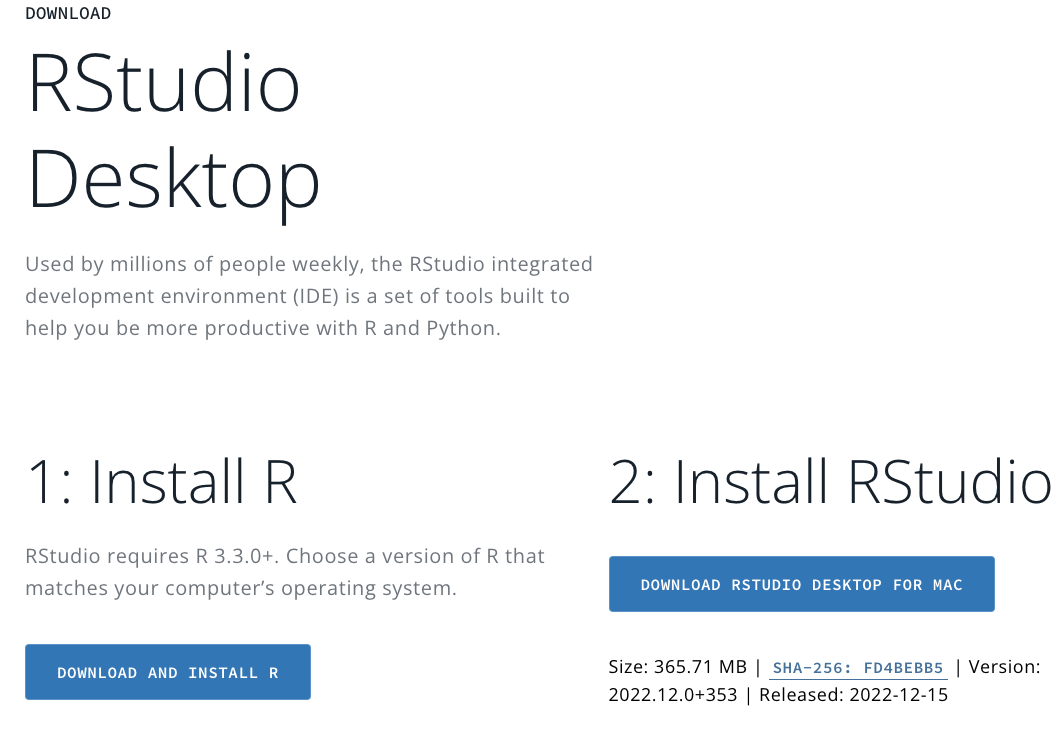
\includegraphics[width=14.71in]{images/2.1rdownload} \caption{Download screen for R and RStudio}\label{fig:unnamed-chunk-2}
\end{figure}

We want to install \textbf{R} before we install \textbf{RStudio}

Once you have downloaded both \textbf{R} and \textbf{RStudio} you can load up the \textbf{RStudio IDE} and it will come up with something like this.

\begin{figure}
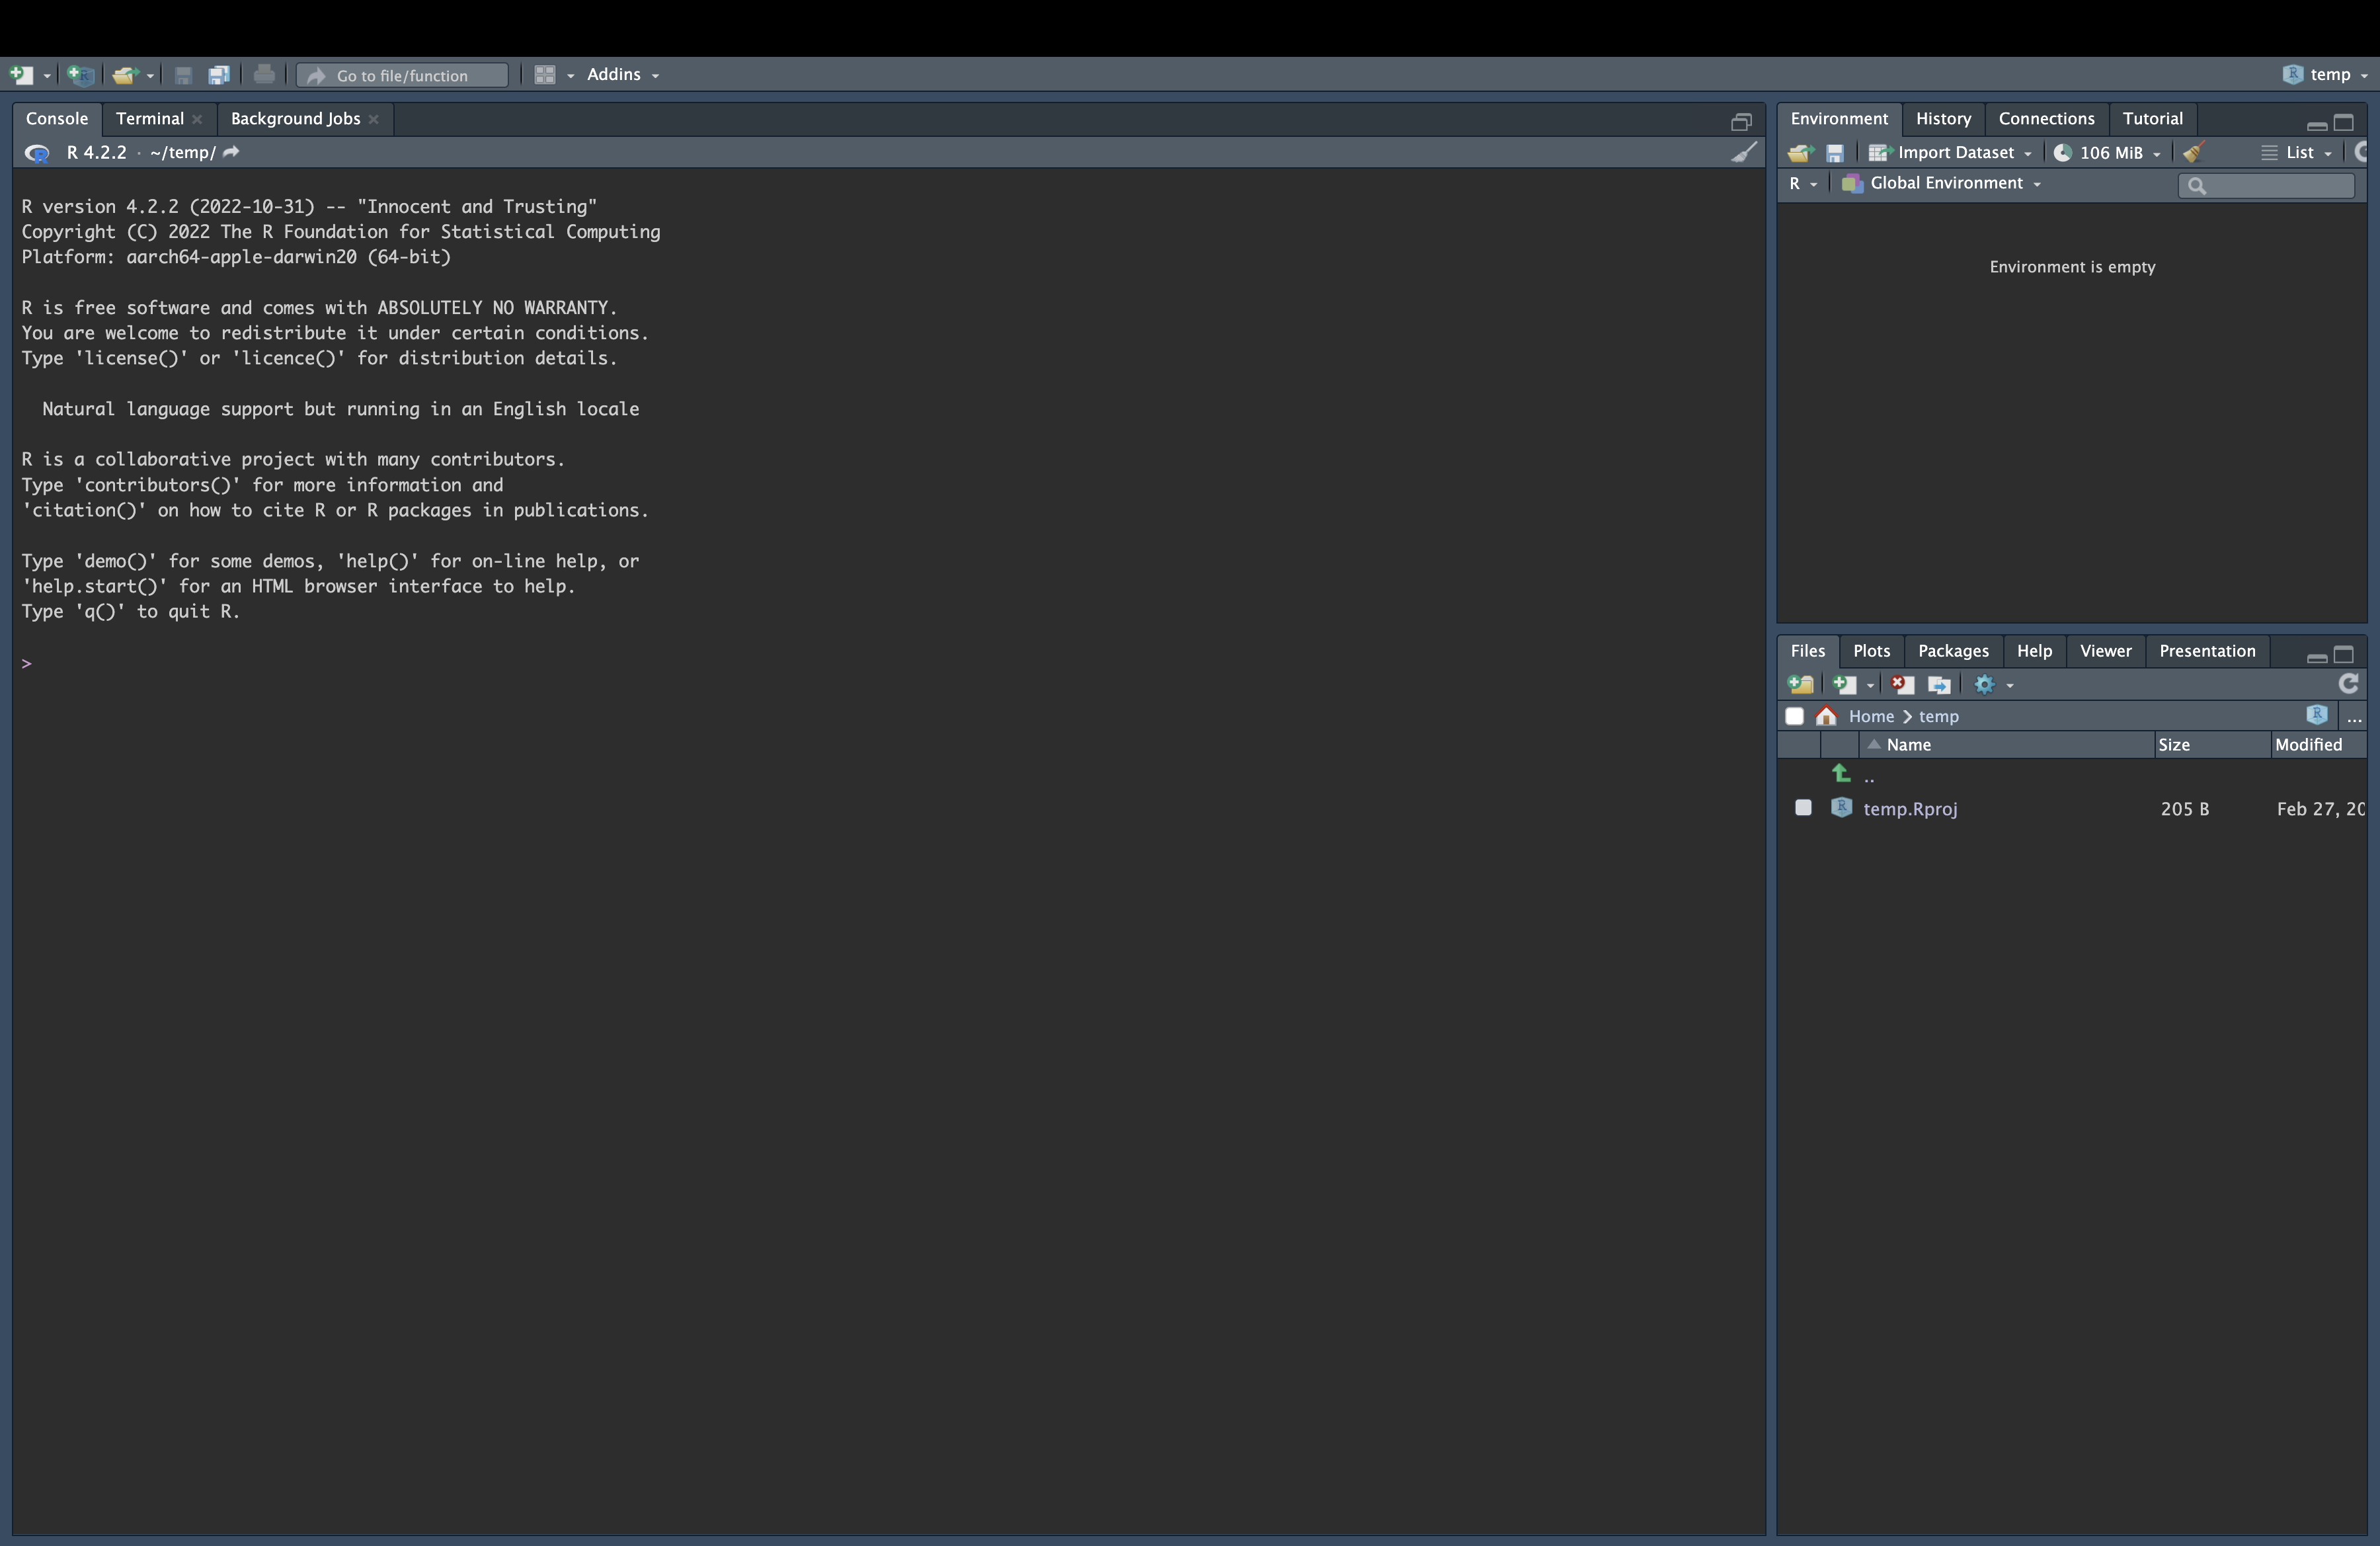
\includegraphics[width=50in]{images/2.3rstudio} \caption{RStudio IDE}\label{fig:unnamed-chunk-3}
\end{figure}

\hypertarget{creating-a-project}{%
\subsection{Creating a Project}\label{creating-a-project}}

Every time we want to work on something new, we should make a \texttt{New\ Project} to keep things organized. This will be a folder where all your code and output will be stored.

To create a new project we will go to `\texttt{File\ -\textgreater{}\ New\ Project}

\begin{figure}
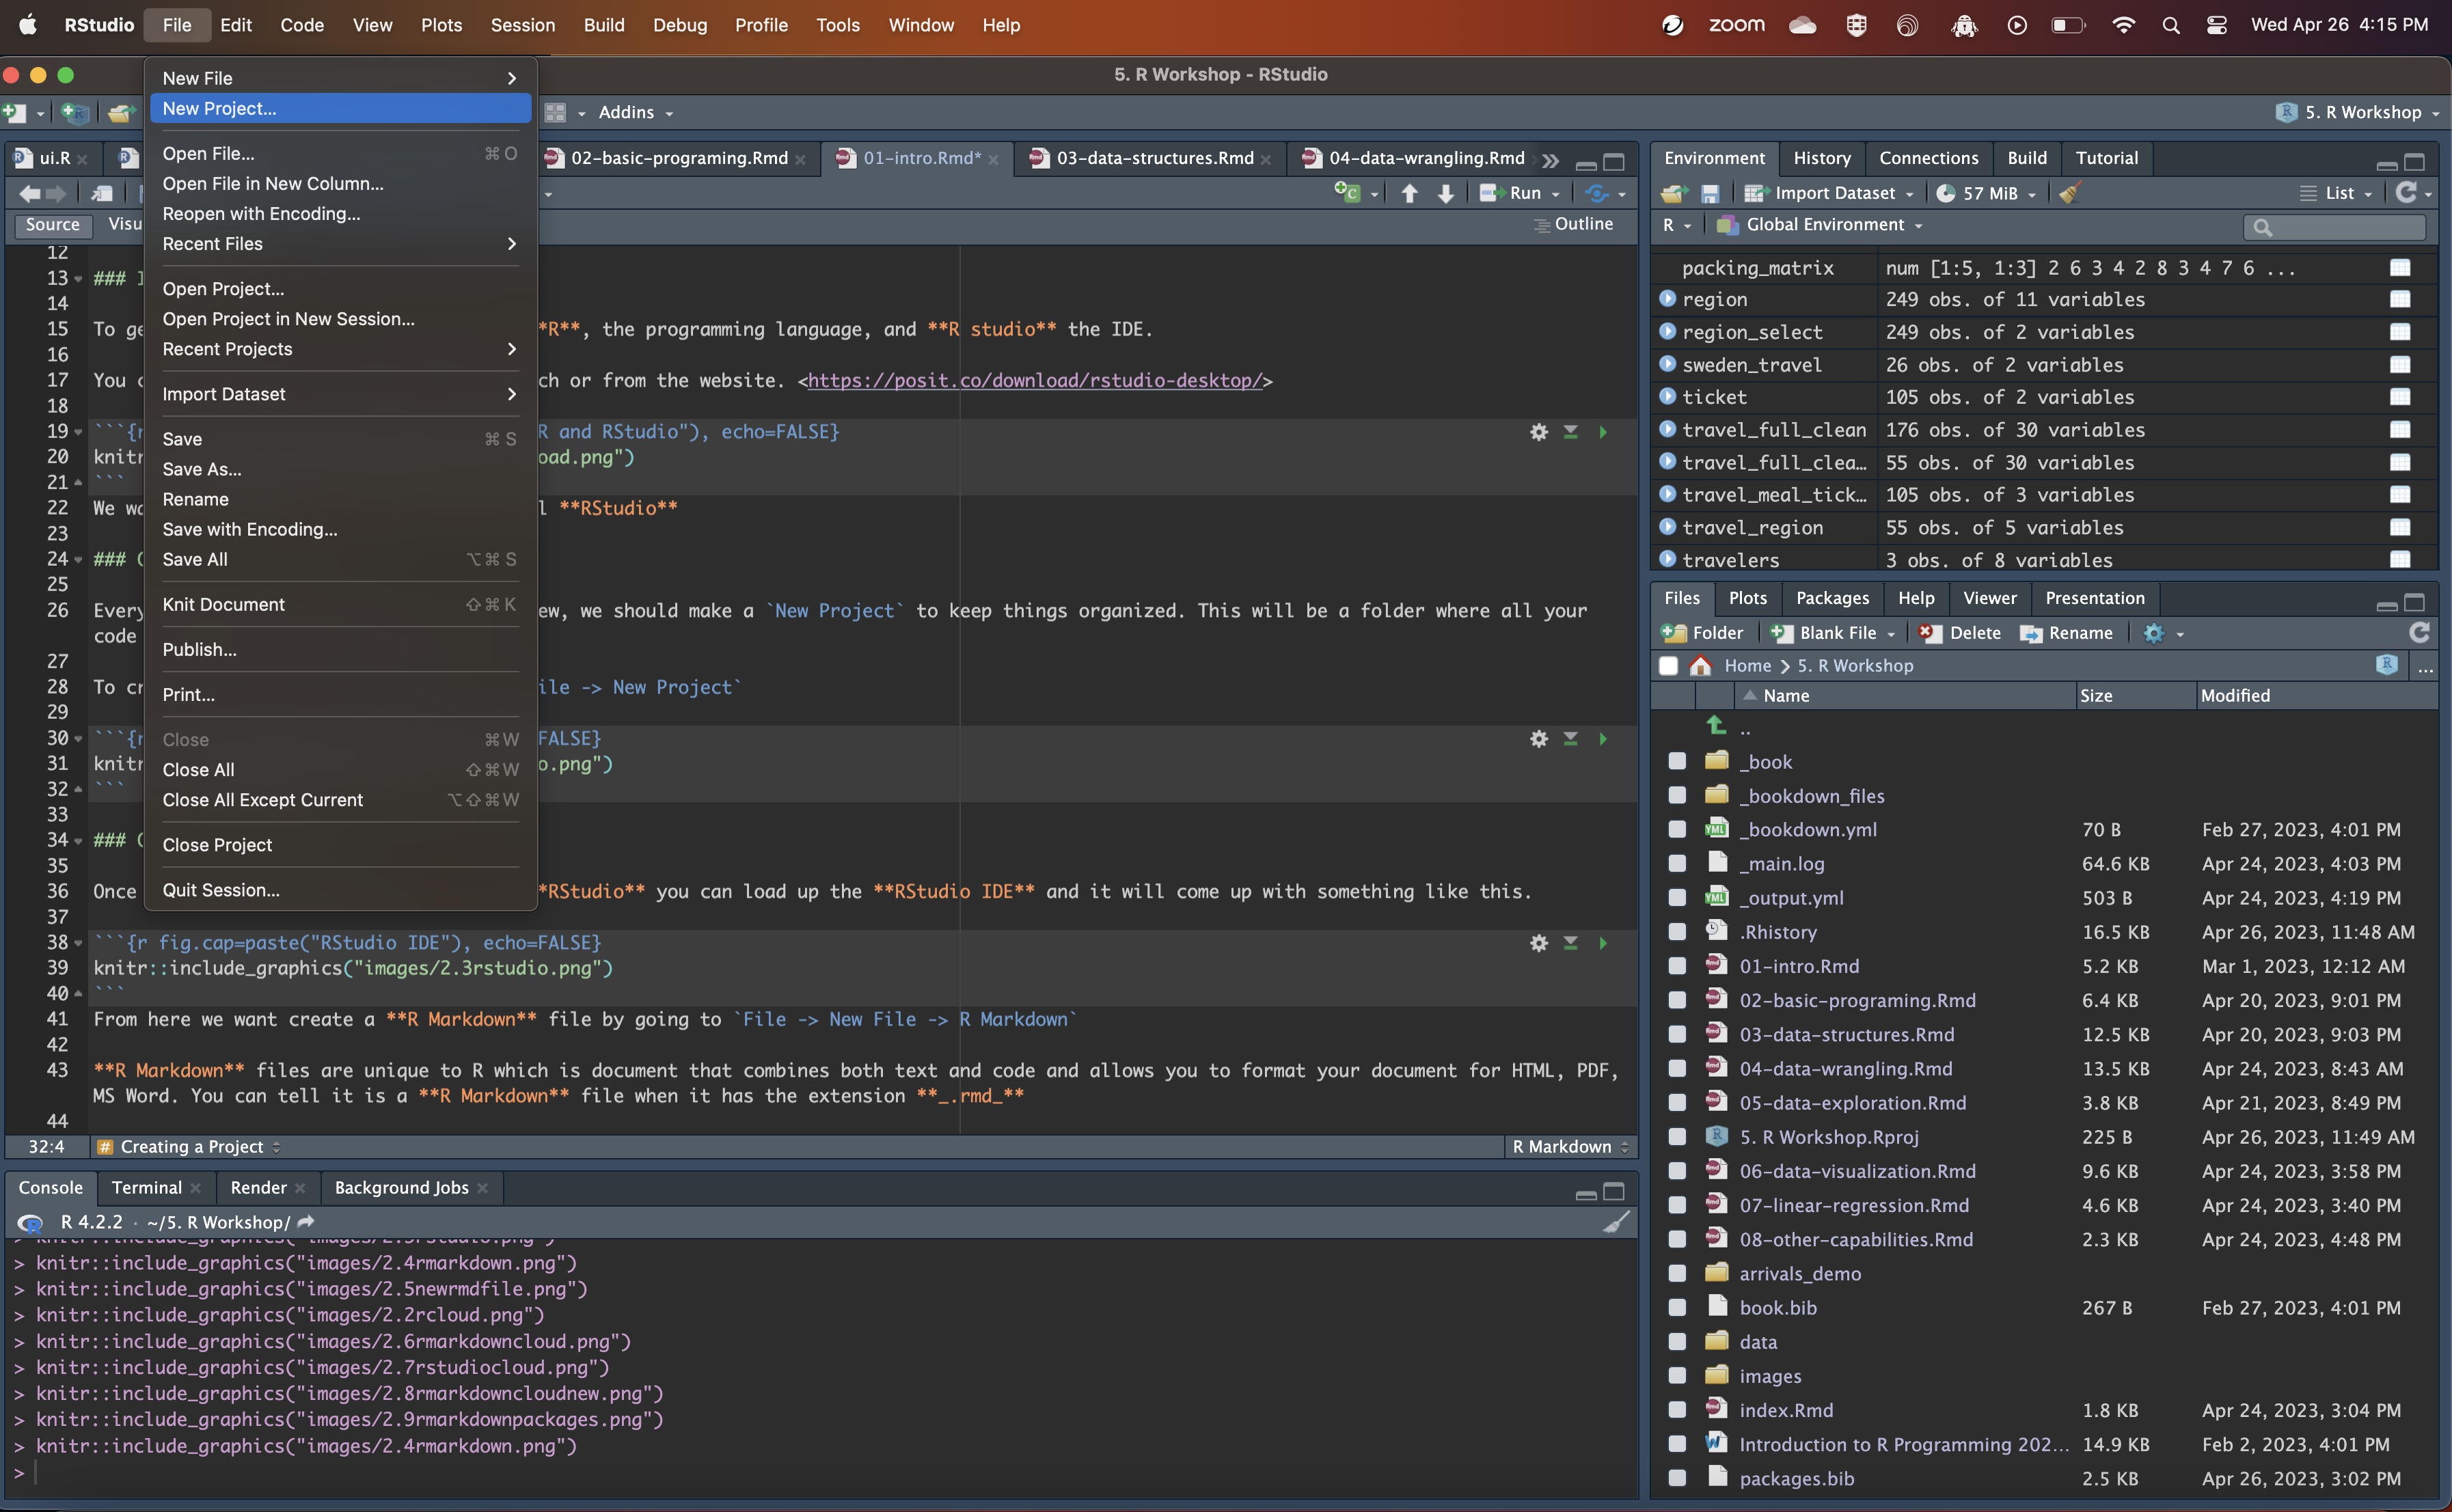
\includegraphics[width=49.83in]{images/2.10newproject} \caption{New}\label{fig:unnamed-chunk-4}
\end{figure}

After selecting \textbf{New Project}, select \textbf{New Directory} and then select \textbf{New Project}. You will then get a window that lets you type in a directory name and allows you to select a location for this folder.

\begin{figure}
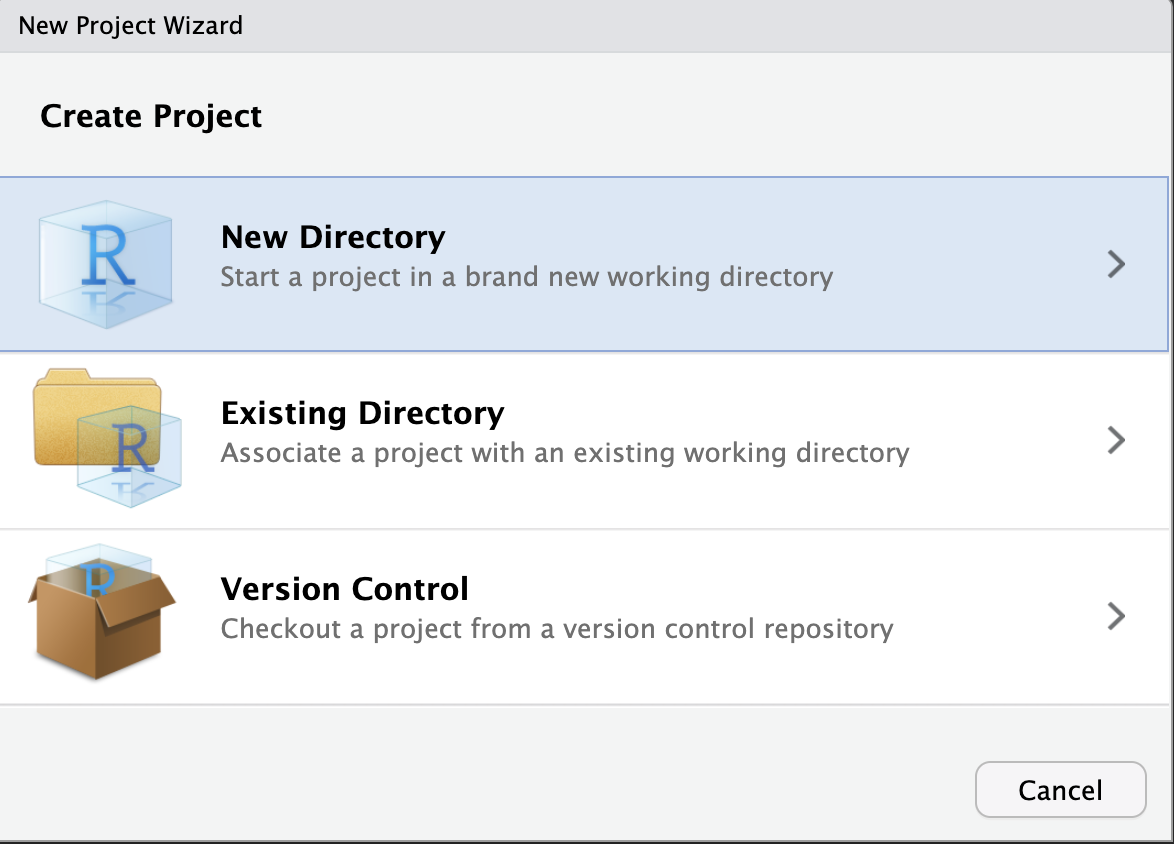
\includegraphics[width=16.31in]{images/2.11newproject1} \caption{Creating new project}\label{fig:unnamed-chunk-5-1}
\end{figure}
\begin{figure}
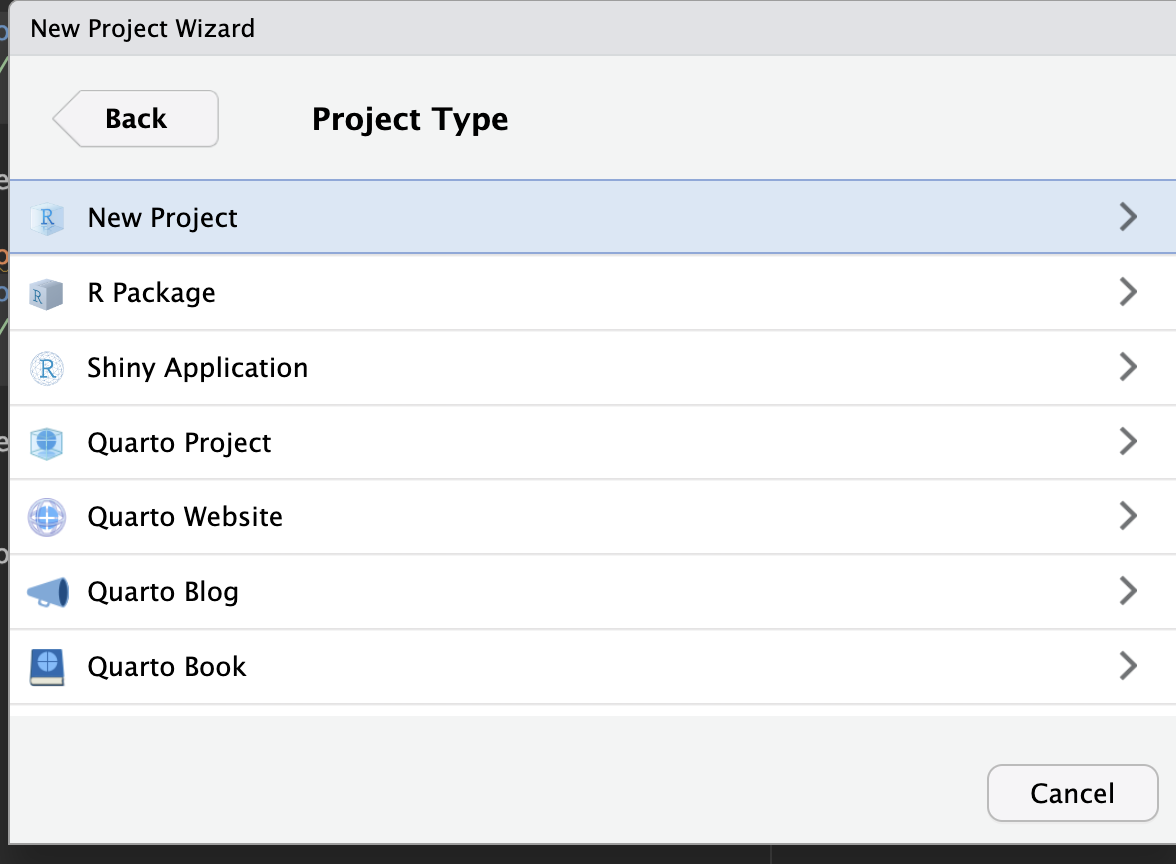
\includegraphics[width=16.33in]{images/2.12newproject2} \caption{Creating new project}\label{fig:unnamed-chunk-5-2}
\end{figure}
\begin{figure}
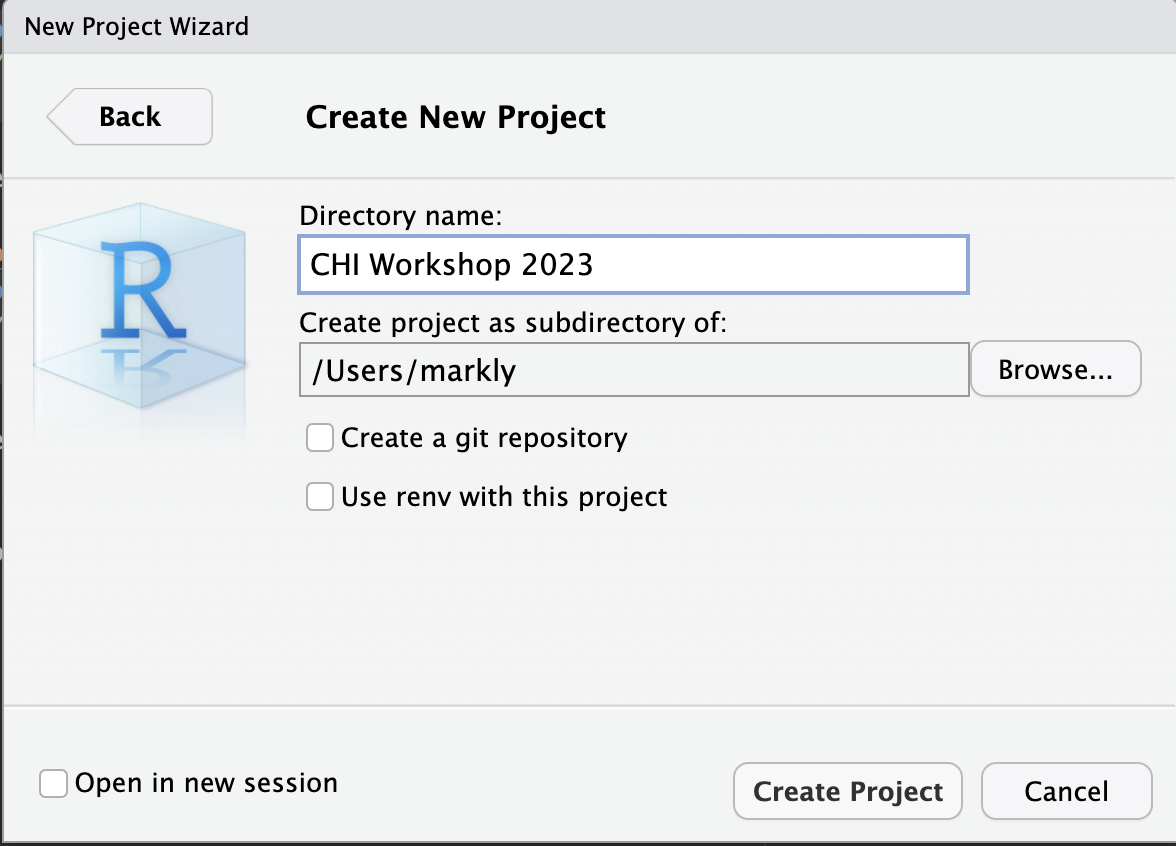
\includegraphics[width=16.33in]{images/2.13newproject3} \caption{Creating new project}\label{fig:unnamed-chunk-5-3}
\end{figure}

Once we created the new project folder, we can create a new folder in there to hold our data. This will be more clear when we start loading our datasets.

Now that everything is set up, we will start by making our first R-markdown file, which is a file format that allows you to write reports and as well with chunks of code.

\hypertarget{creating-.rmd-file}{%
\subsection{Creating .RMD file}\label{creating-.rmd-file}}

Now that we have created our new project and added our data to the folder, we can create our first \textbf{R Markdown} file by going to \texttt{File\ -\textgreater{}\ New\ File\ -\textgreater{}\ R\ Markdown}

\textbf{R Markdown} files are unique to R which is document that combines both text and code and allows you to format your document for HTML, PDF, MS Word. You can tell it is a \textbf{R Markdown} file when it has the extension \textbf{\emph{.rmd}}

A popup window should come up and we need to title our \textbf{R Markdown} file.

You can type in \textbf{\emph{2023 Rworkshop}} for the title and then click on ok to create the \textbf{\emph{.rmd}} file.

\begin{figure}
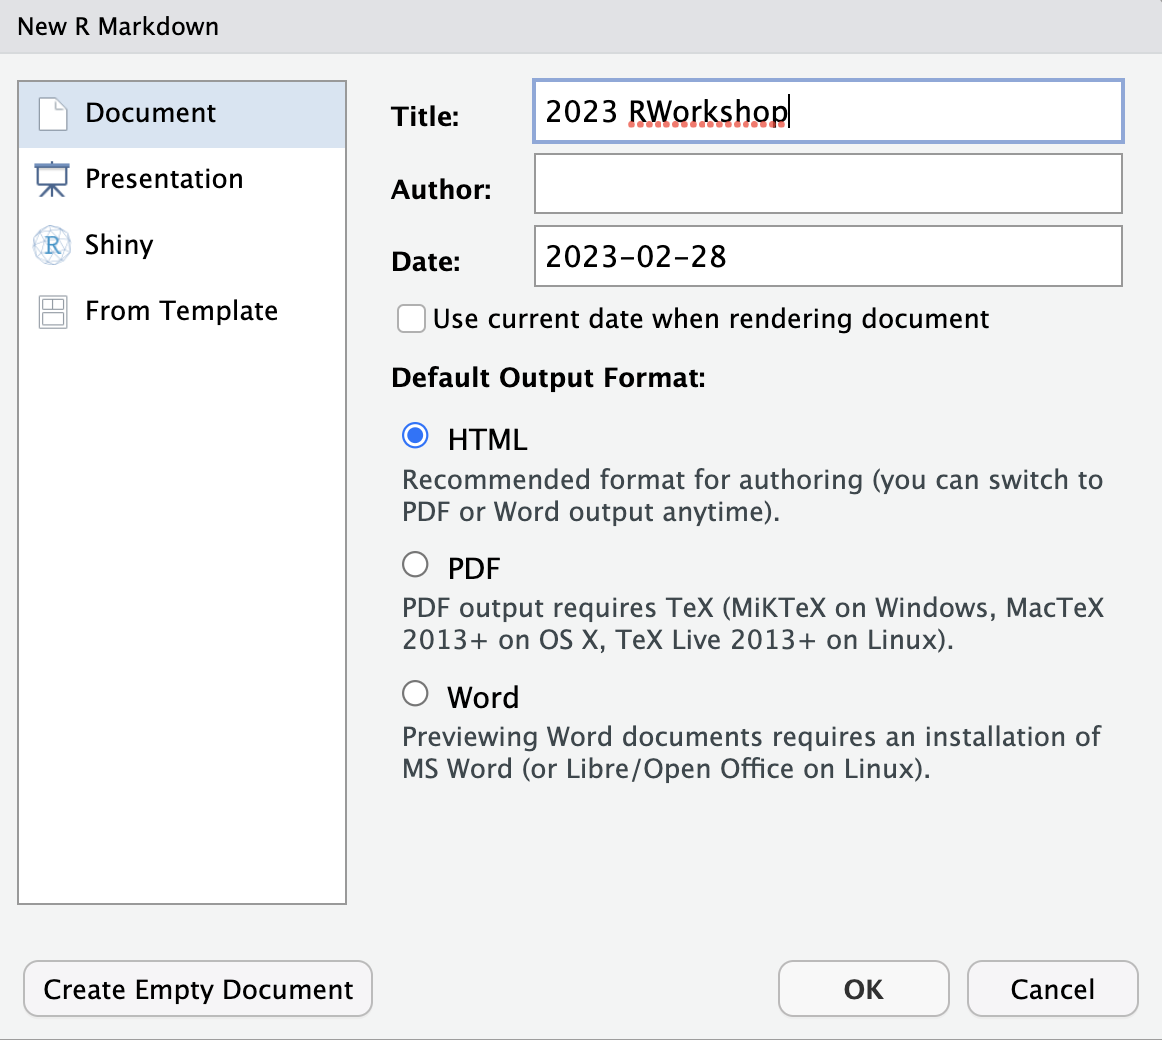
\includegraphics[width=16.14in]{images/2.4rmarkdown} \caption{RStudio markdown creation}\label{fig:unnamed-chunk-6}
\end{figure}

Once you hit \texttt{OK}, you should see a tab at the top that says \texttt{Untitled1} and your \textbf{RStudio IDE} should have 4 distinct panels.

\begin{figure}
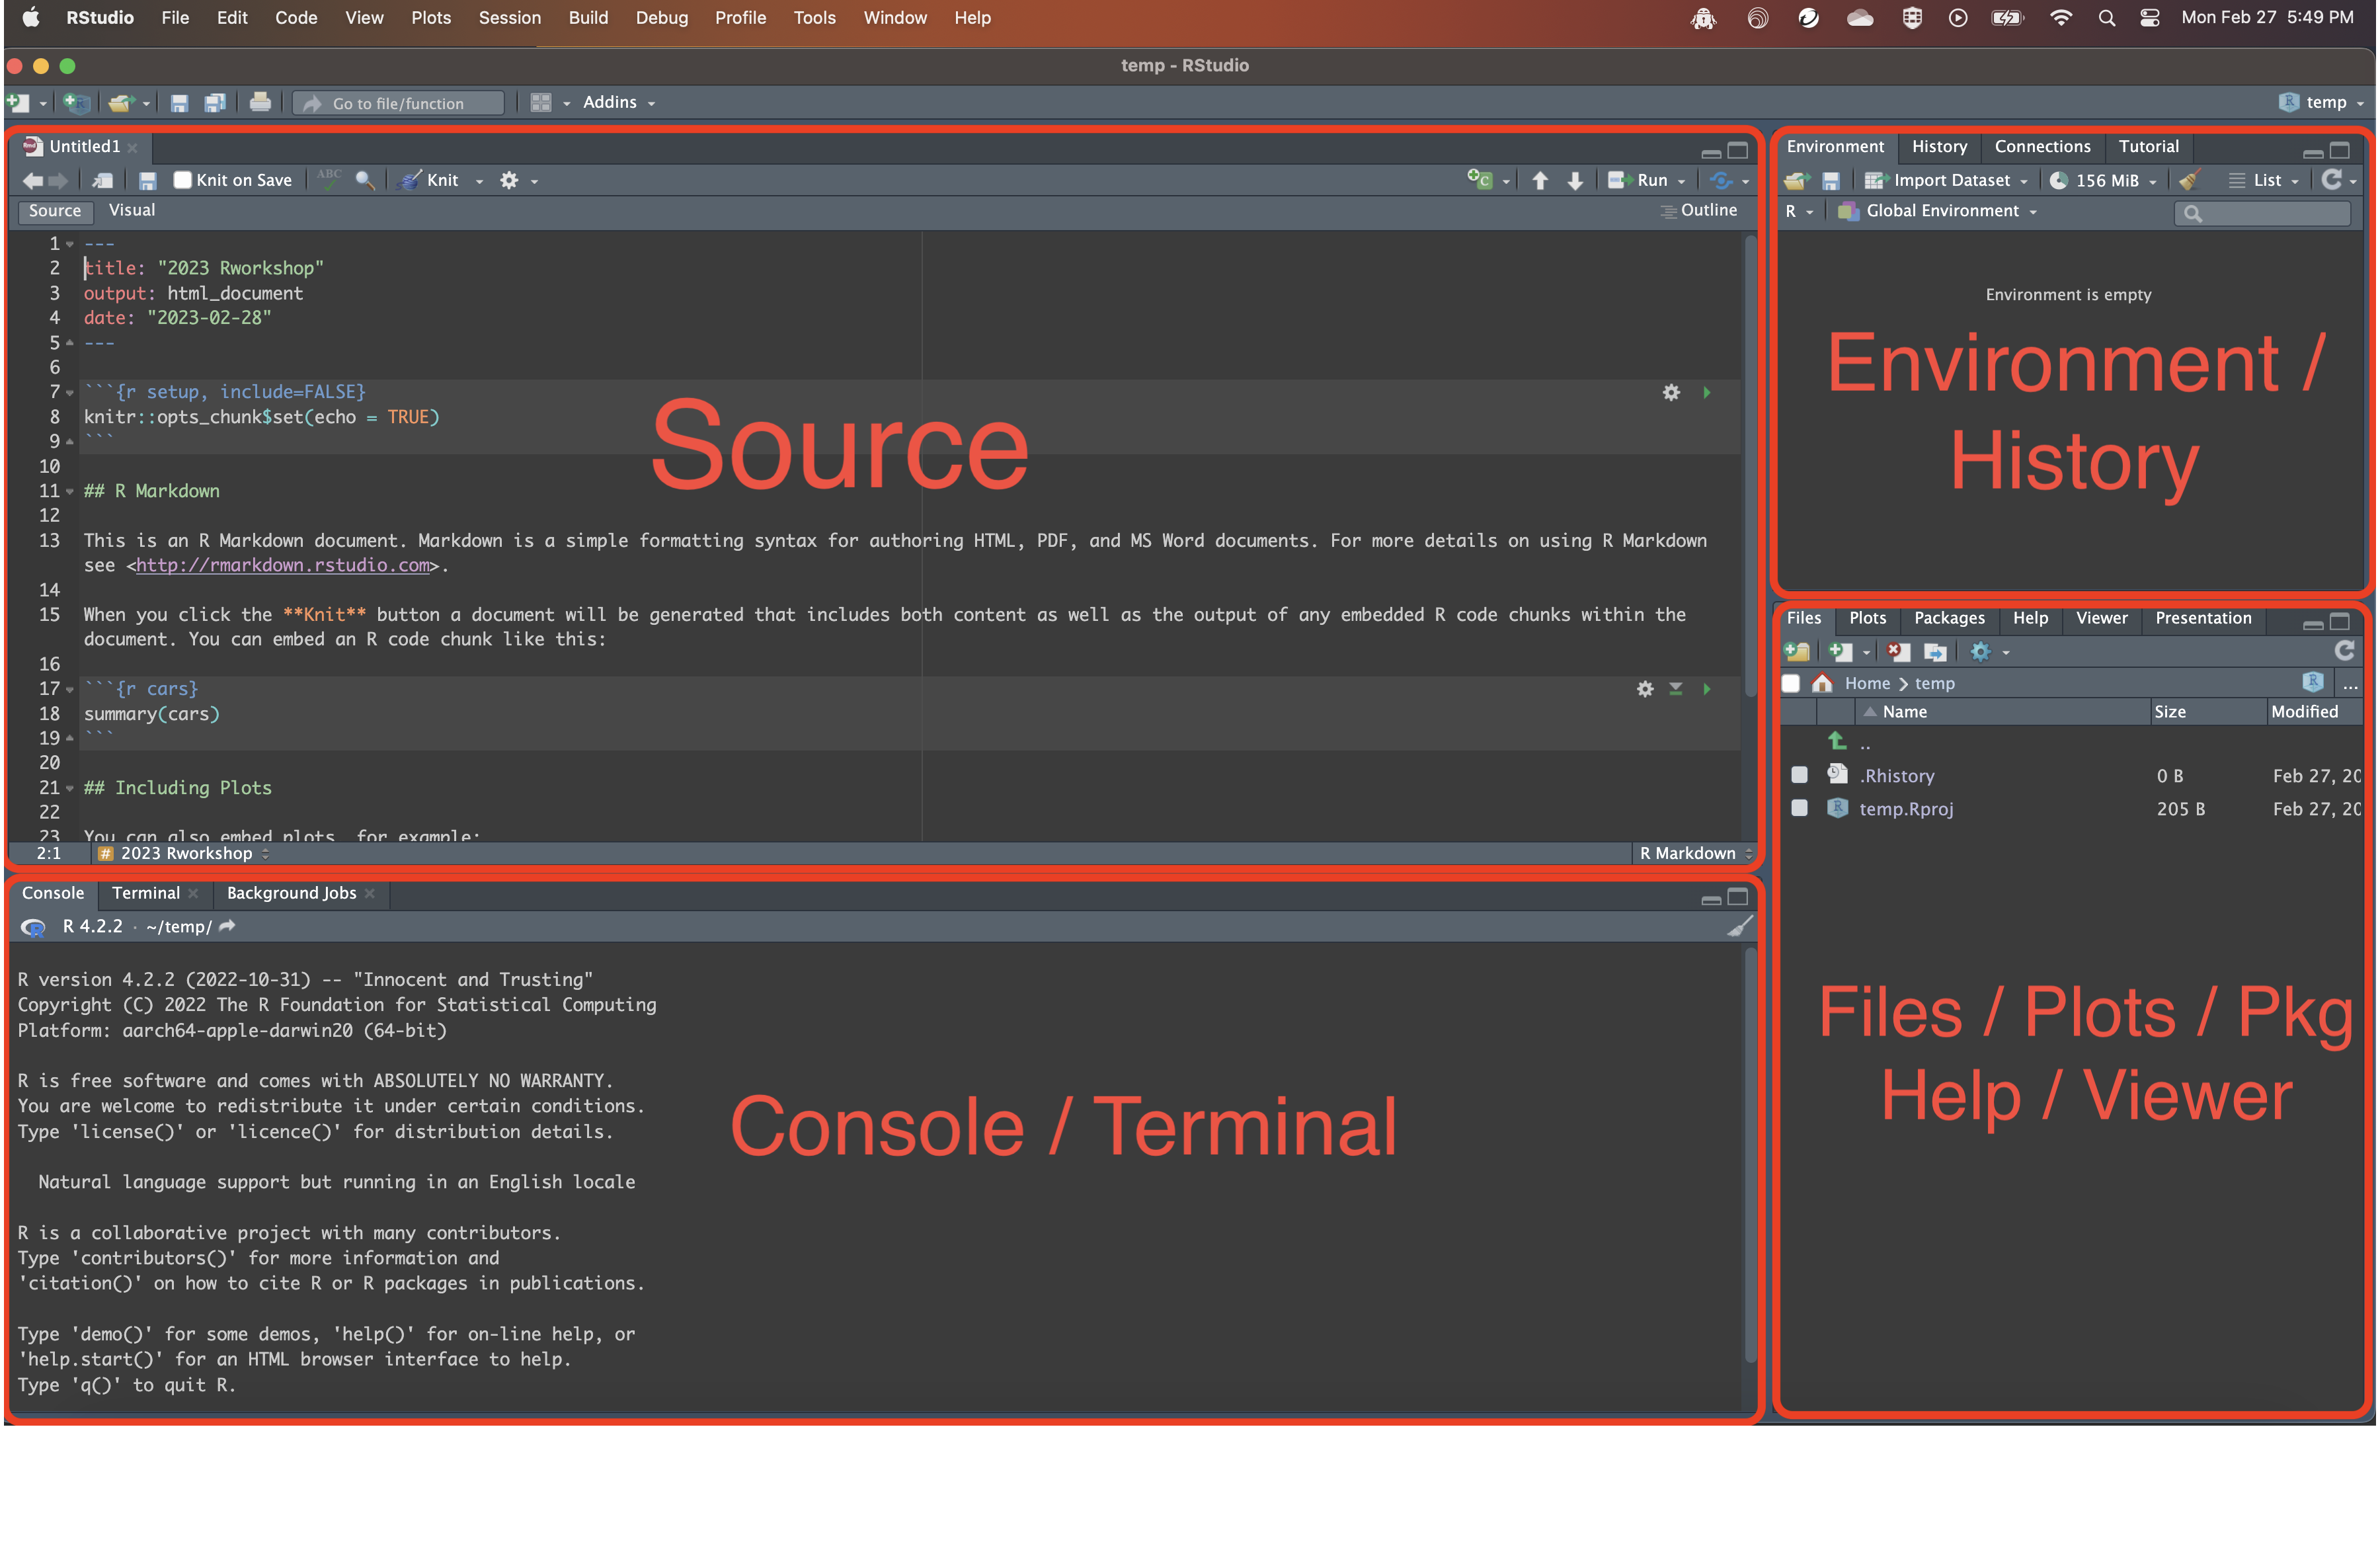
\includegraphics[width=50in]{images/2.5newrmdfile} \caption{New .rmd file}\label{fig:unnamed-chunk-7}
\end{figure}

\begin{enumerate}
\def\labelenumi{\arabic{enumi}.}
\item
  Source - Places where most of the coding happens. The source can look different depending the type of file you are working with (.rmd, .R, .MD). Any dataset you want to view will also show up in this window.
\item
  Environment/History - This is were you can find any stored variables (objects), imported scripts, loaded databases that are defined in memory. The history tab will contain a history of all the R commands that you have executed in this session
\item
  Console/Terminal - This is were the commands that are written in the source window are actually executed and started to run. This would be the same if you were to use R using a command line instead of an IDE. You can run and enter in commands and scripts in this window, but they will be executed as soon as you hit \texttt{ENTER/RETURN}. Can be used to quickly check a snip of code, do some basic calculations or install some packages. Runtime errors will also show up in this window which can be useful when you are debugging.
\item
  Files/Plots/Pkgs/Help/Viewer - This is more a directory window where you can cycle between files, plots, packages, help, and Viewer.
\end{enumerate}

\hypertarget{getting-started-cloud}{%
\section{Getting Started (Cloud)}\label{getting-started-cloud}}

If you would like to use the cloud version of \textbf{RStudio} you can sign up for the free version here:

\url{https://posit.cloud/plans/free}

\begin{figure}
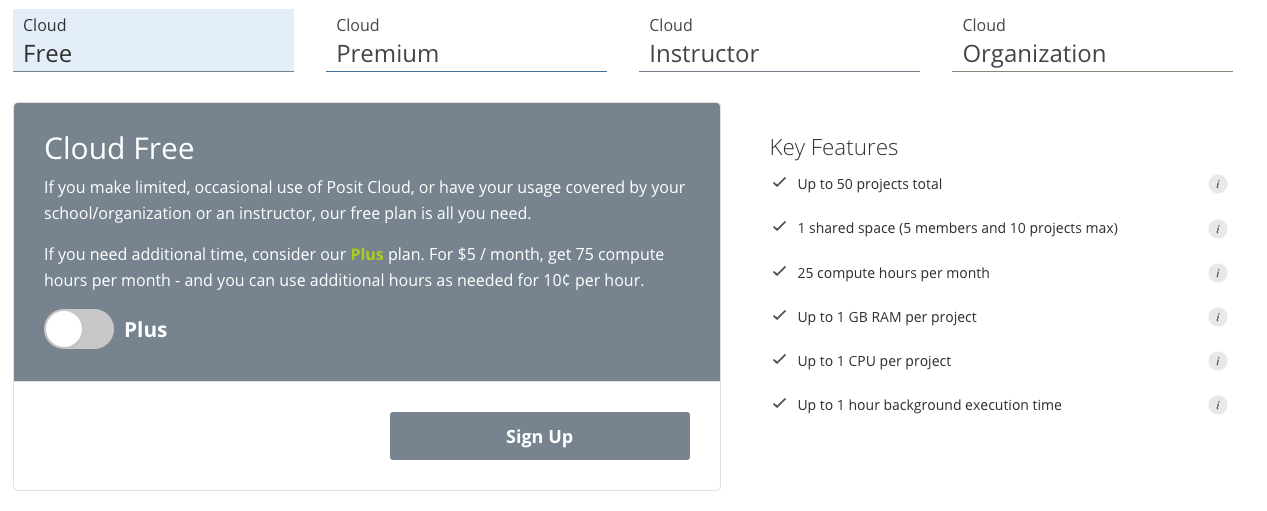
\includegraphics[width=17.6in]{images/2.2rcloud} \caption{Sign up for RStudio cloud}\label{fig:unnamed-chunk-8}
\end{figure}

If you are just planning to use R occasionally and don't need heavy computing, then the free version of RStudio cloud will work just fine.

\hypertarget{creating-.rmd-file-1}{%
\subsection{Creating .RMD File}\label{creating-.rmd-file-1}}

After logging in to the free account, you can click on \texttt{New\ Project} on the right hand side and select \texttt{New\ RStudio\ Project}

\begin{figure}
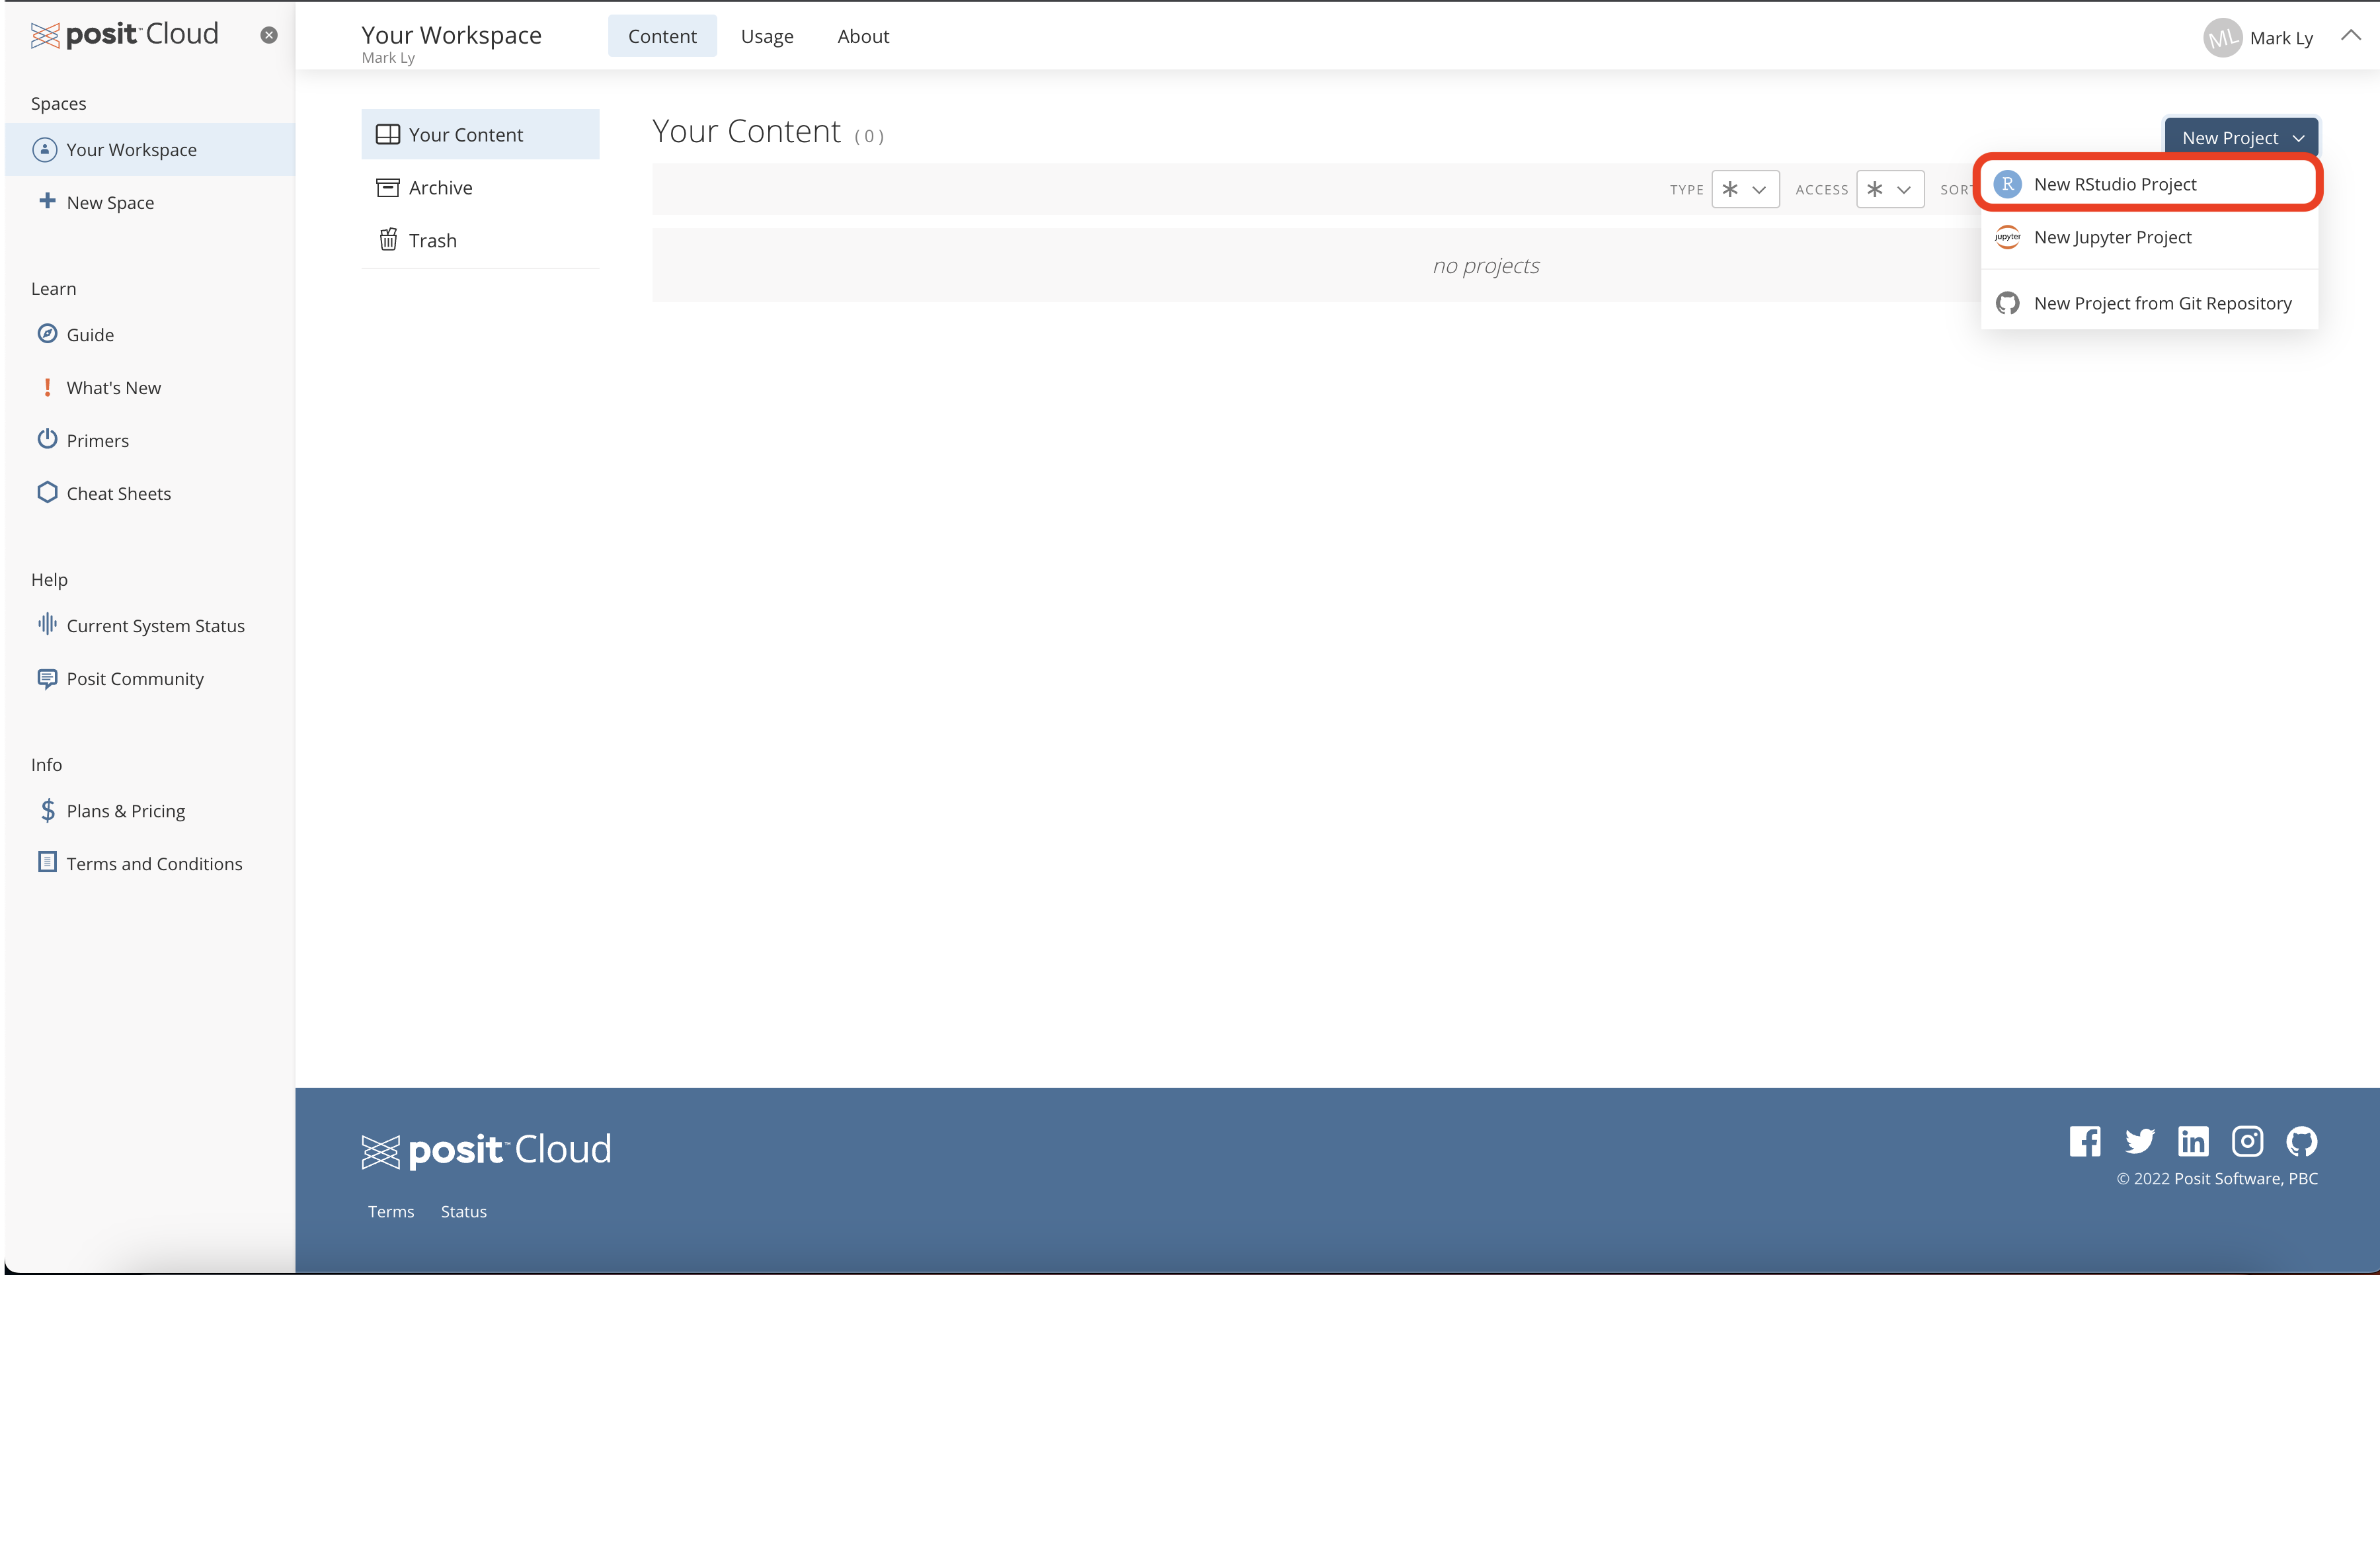
\includegraphics[width=50in]{images/2.6rmarkdowncloud} \caption{RStudio Cloud Creating a new project}\label{fig:unnamed-chunk-9}
\end{figure}

Once you open the new project, you will get a screen similar to this.

\begin{figure}
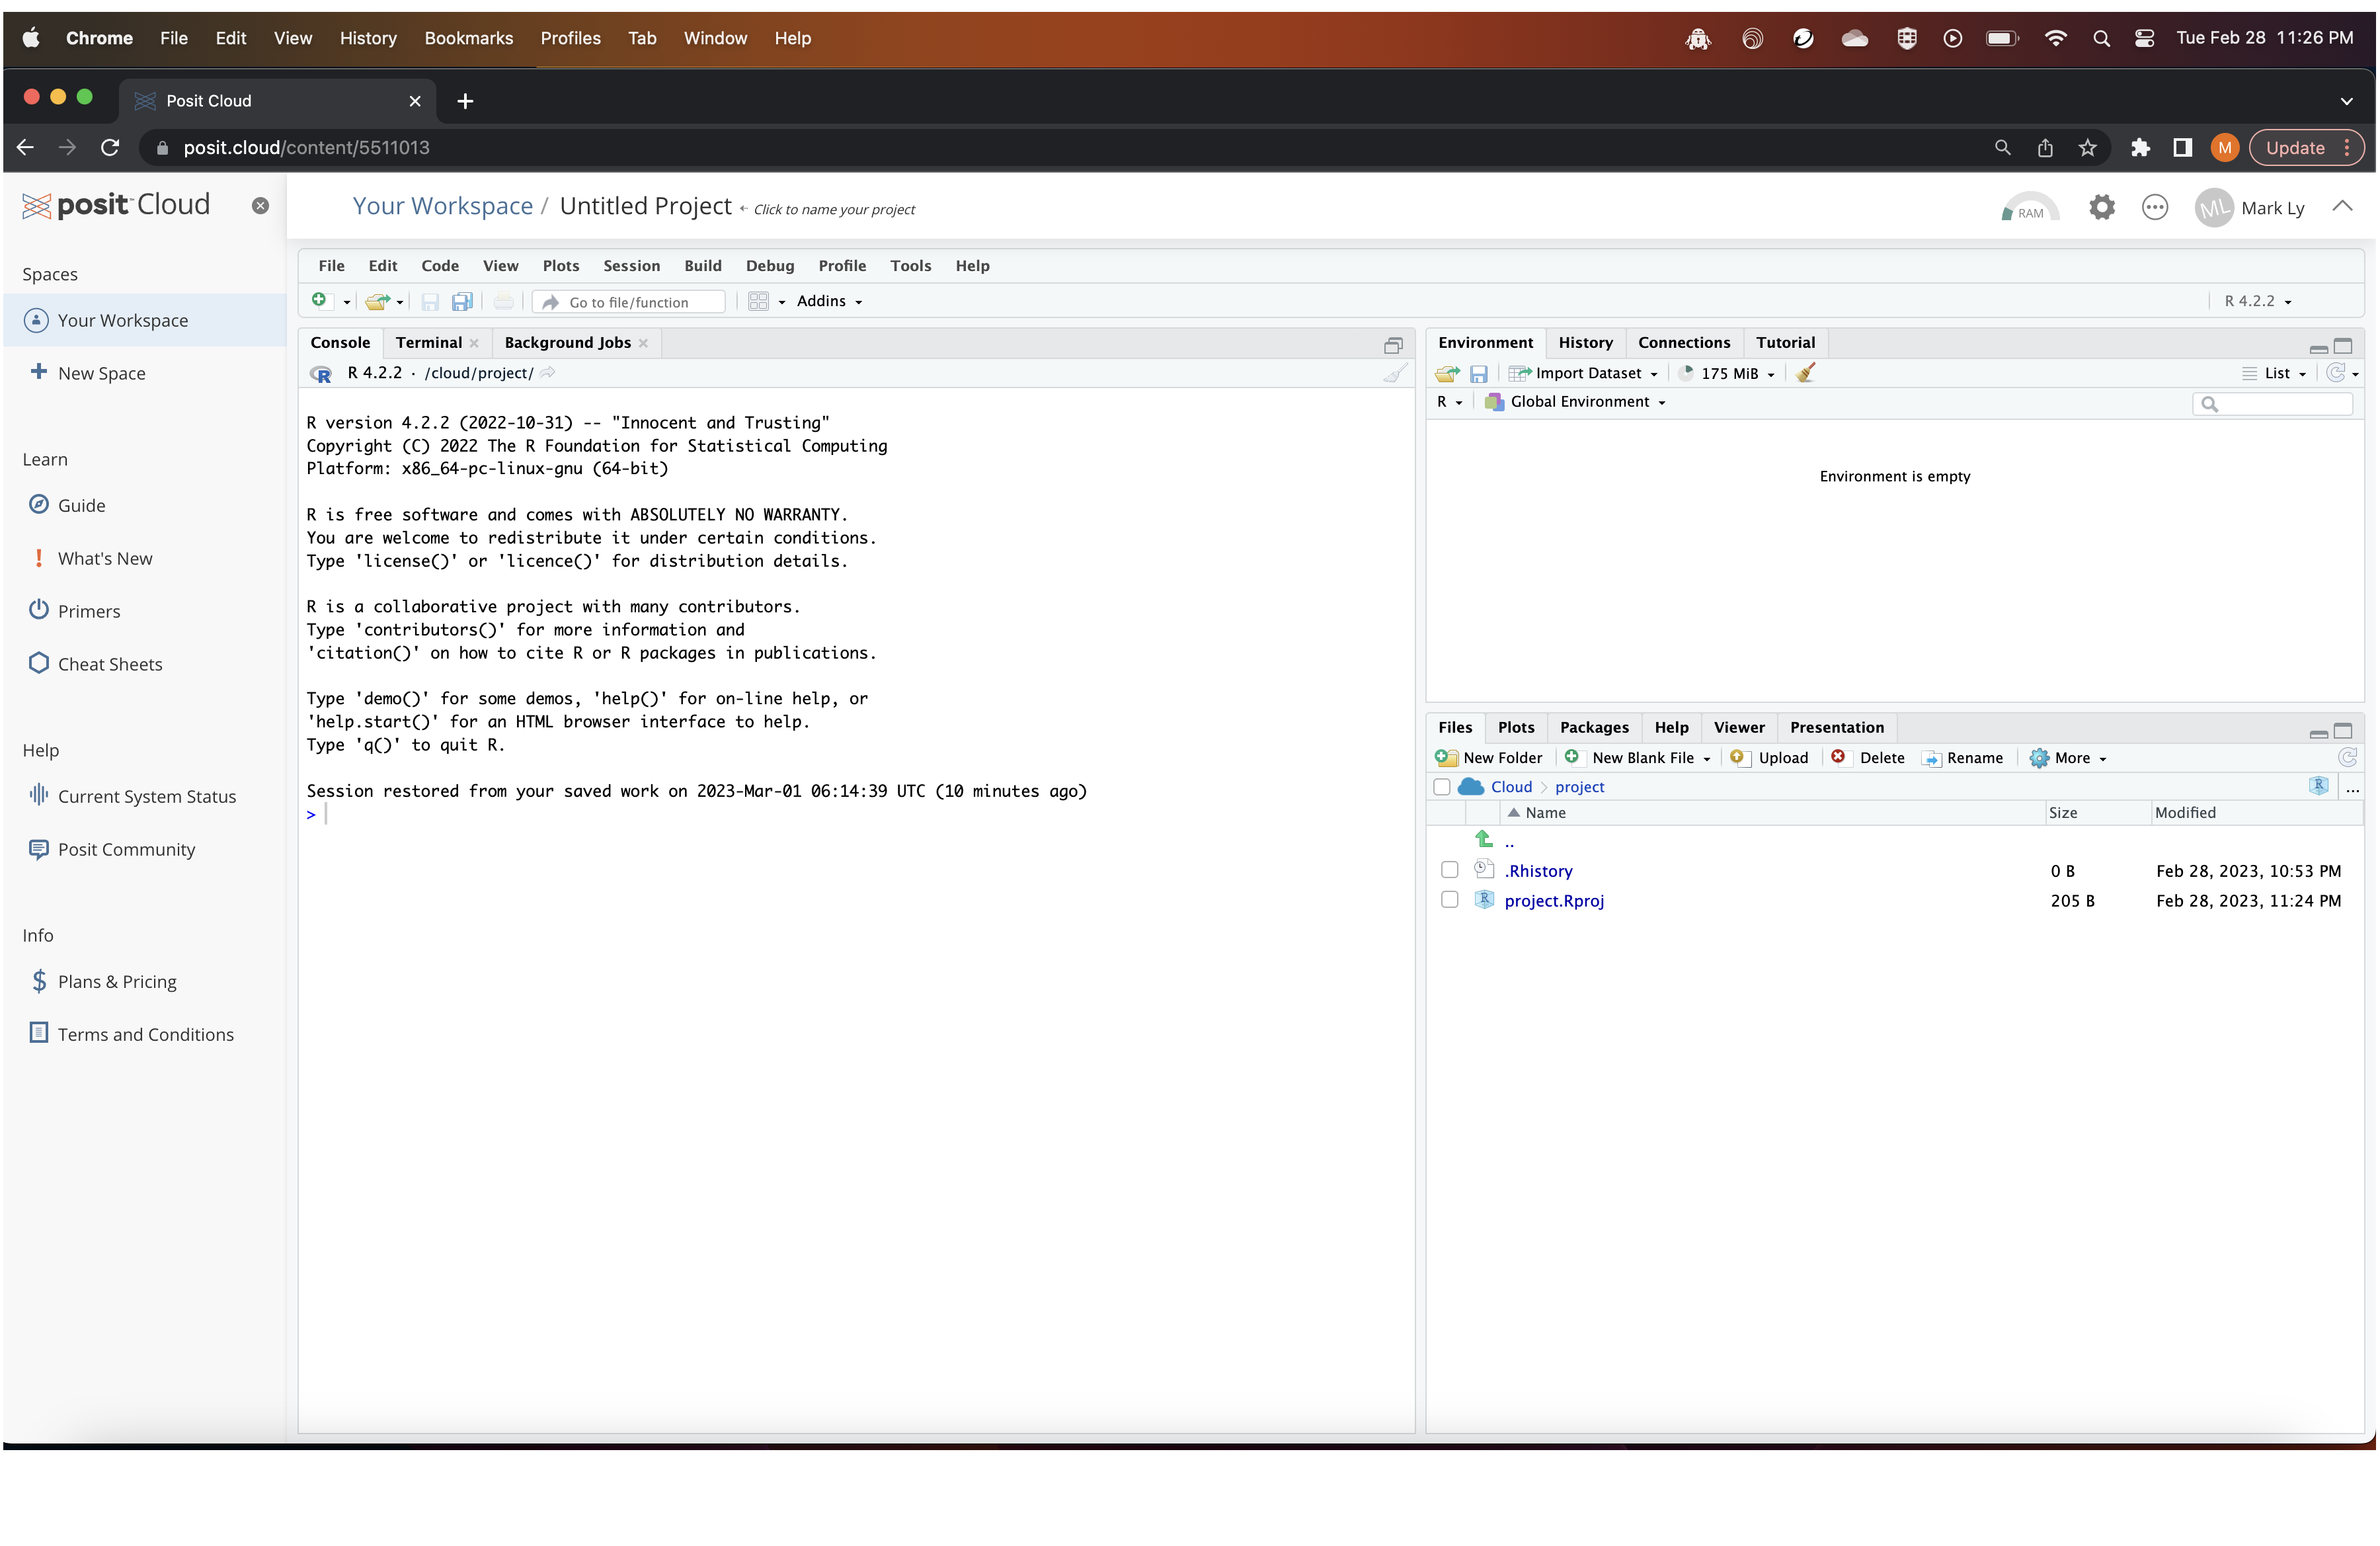
\includegraphics[width=50in]{images/2.7rstudiocloud} \caption{RStudio Cloud Creating a new project}\label{fig:unnamed-chunk-10}
\end{figure}

From here we want create a \textbf{R Markdown} file by going to \texttt{File\ -\textgreater{}\ New\ File\ -\textgreater{}\ R\ Markdown}

\begin{figure}
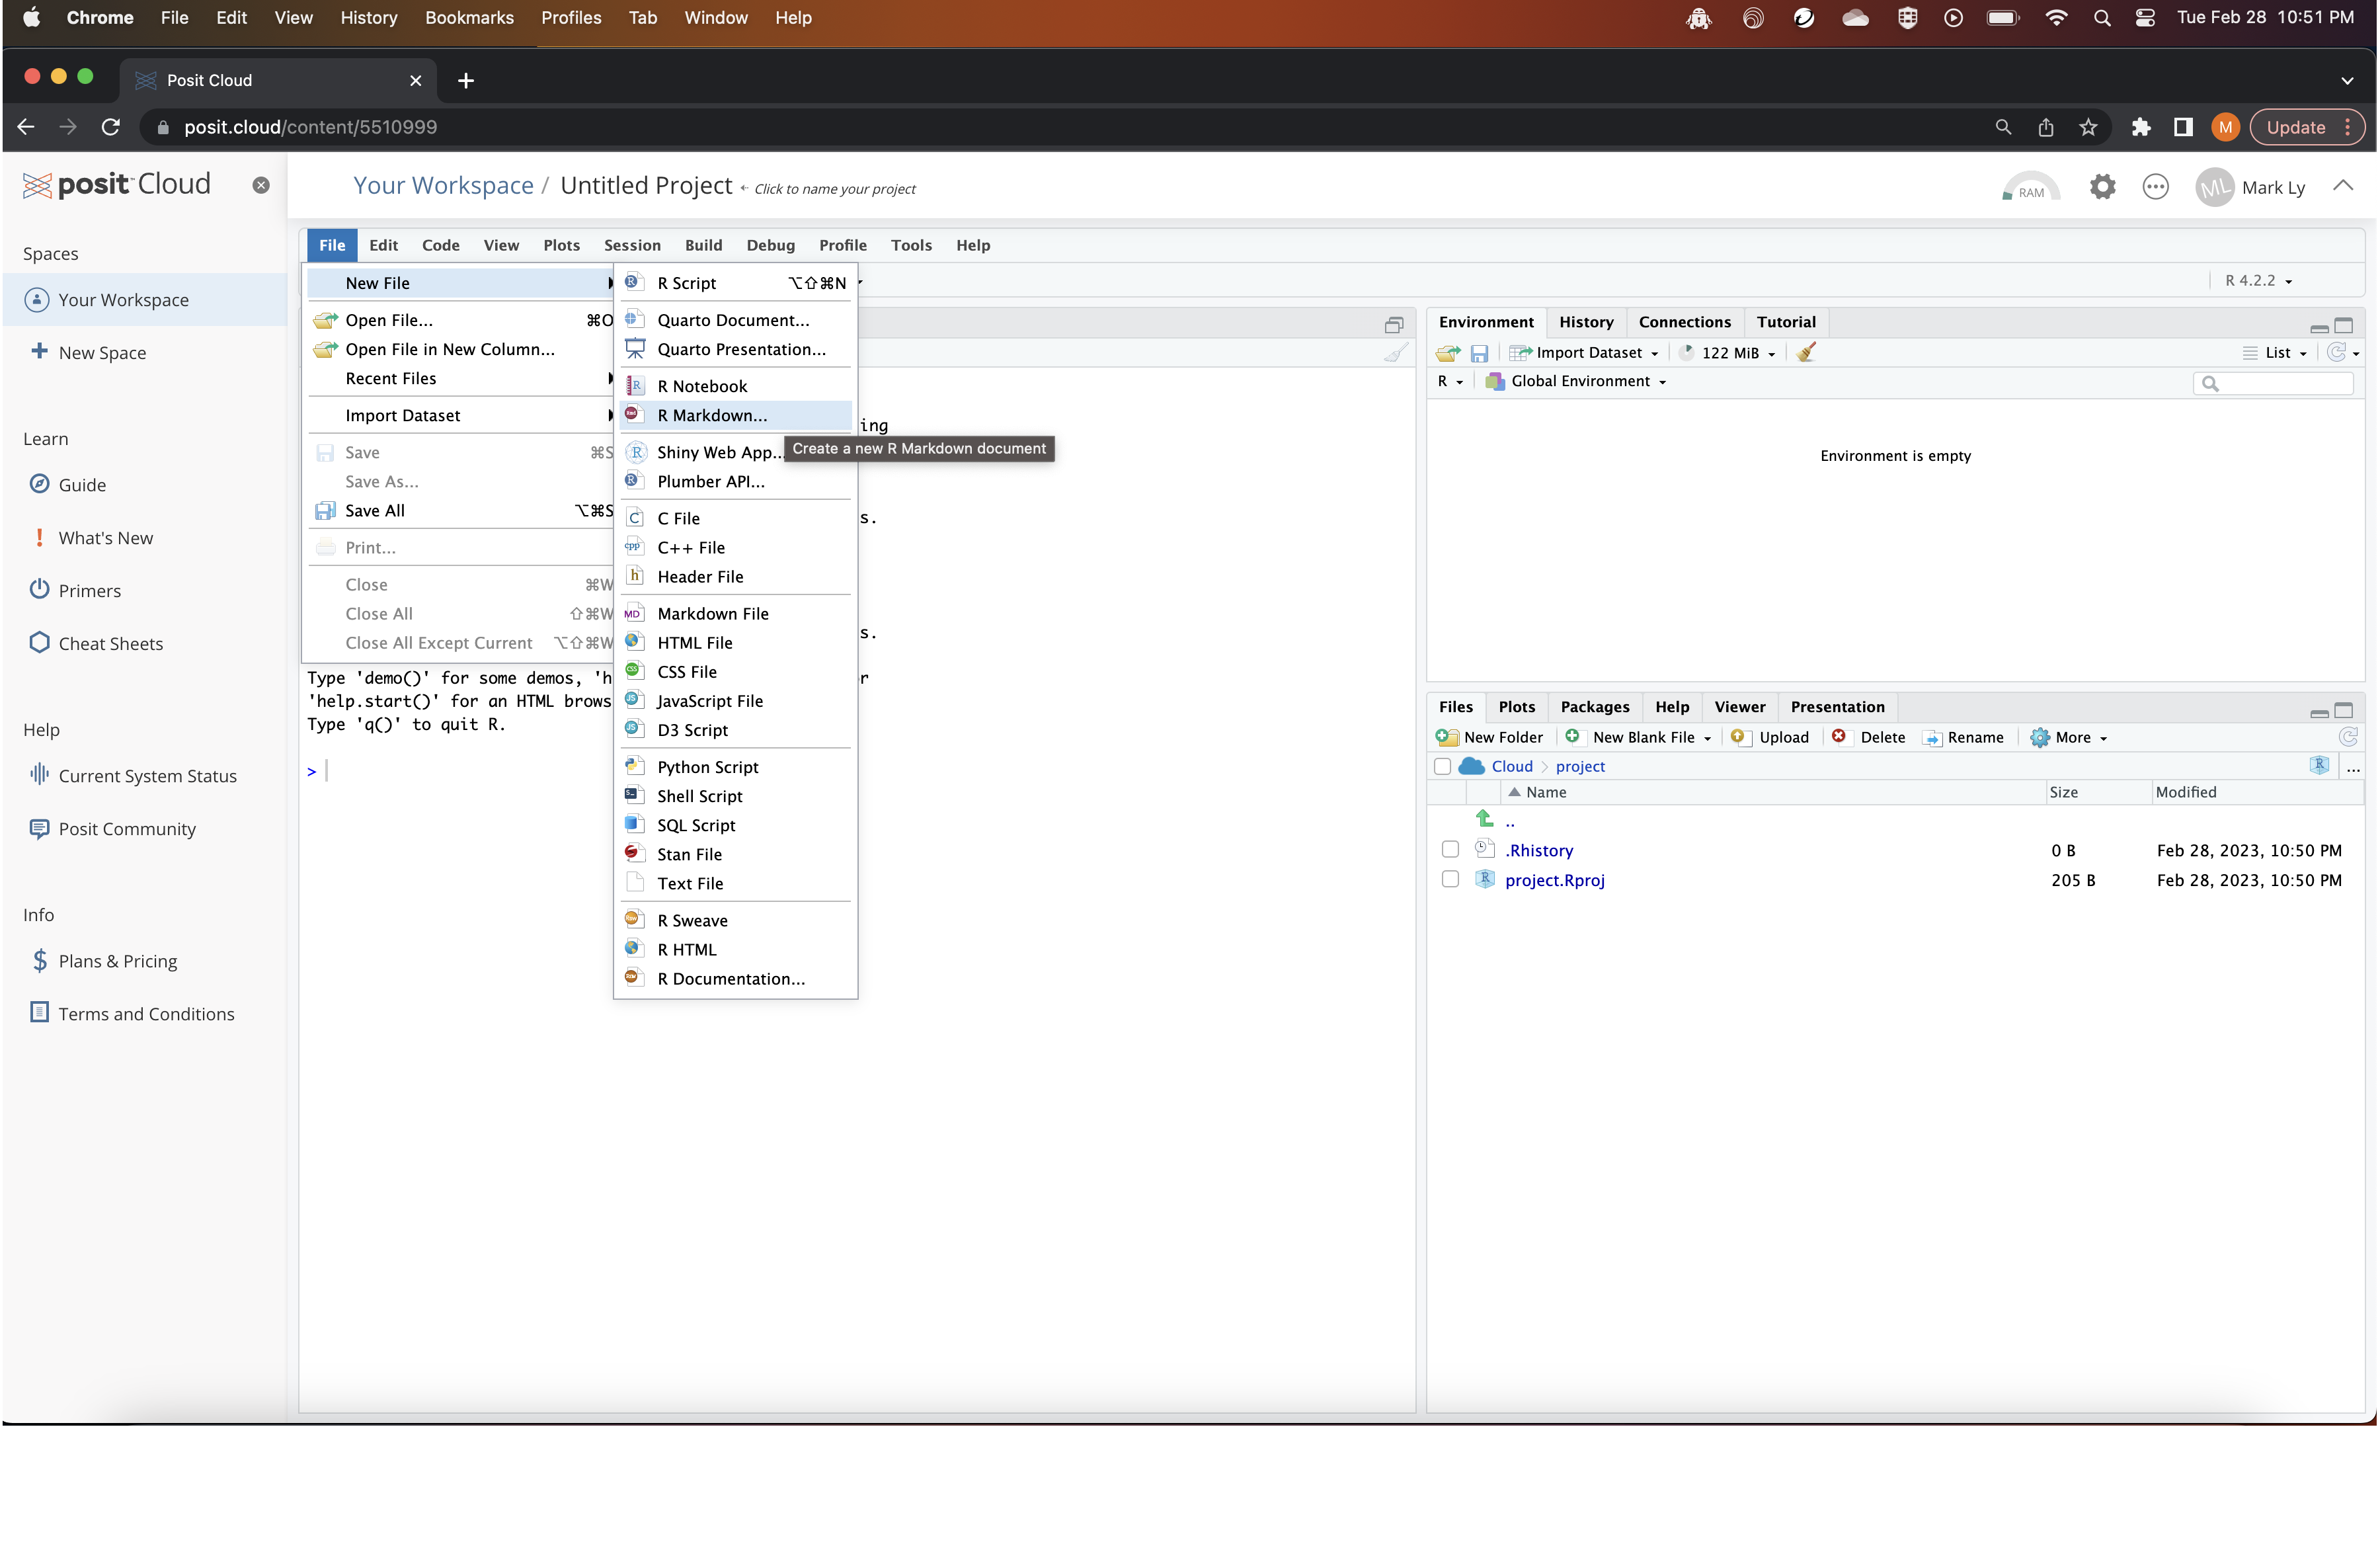
\includegraphics[width=50in]{images/2.8rmarkdowncloudnew} \caption{RStudio Cloud new markdown file}\label{fig:unnamed-chunk-11}
\end{figure}

A pop-up will appear saying it will need to install some packages to create a \textbf{R Markdown} file. You can install these by selecting \texttt{Yes}

\begin{figure}
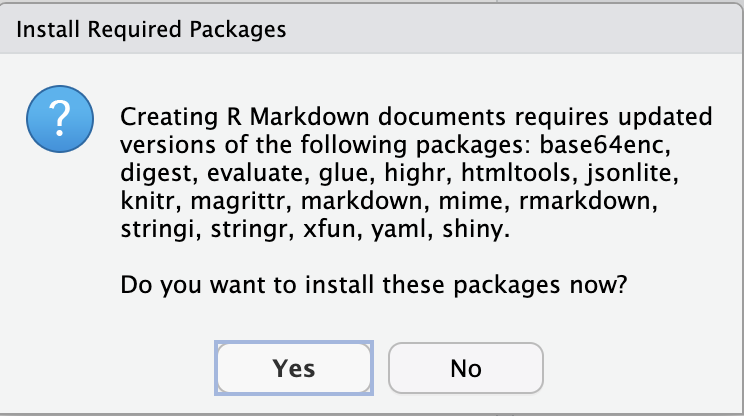
\includegraphics[width=10.33in]{images/2.9rmarkdownpackages} \caption{RStudio cloud markdown packages}\label{fig:unnamed-chunk-12}
\end{figure}

Another popup window should come up and we need to title our \textbf{R Markdown} file.

You can type in \textbf{\emph{2023 Rworkshop}} for the title and then click on ok to create the \textbf{\emph{.rmd}} file.

\begin{figure}
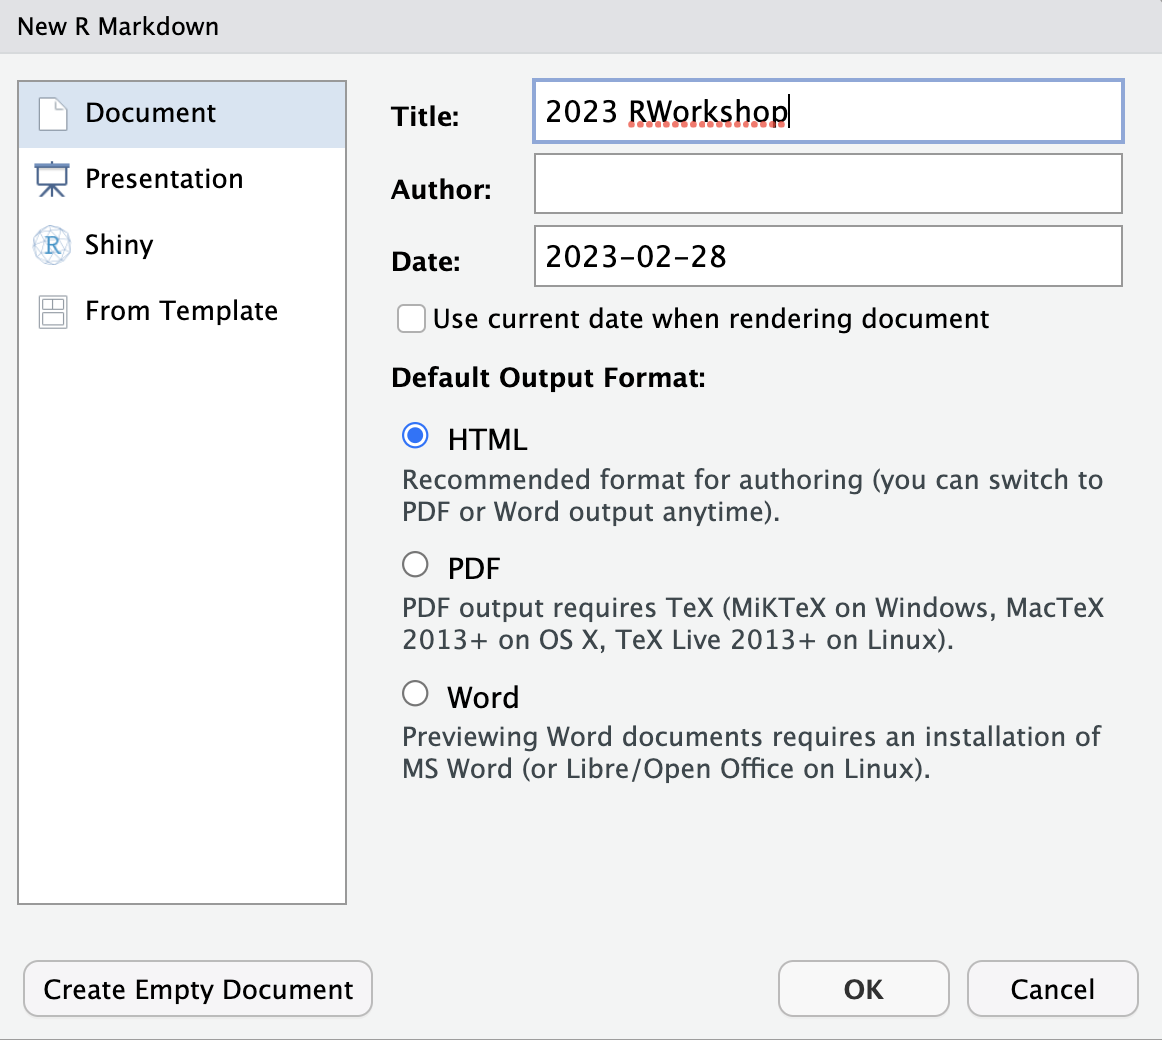
\includegraphics[width=16.14in]{images/2.4rmarkdown} \caption{RStudio cloud markdown name}\label{fig:unnamed-chunk-13}
\end{figure}

Once you hit \texttt{OK}, you should see a tab at the top that says \texttt{Untitled1} and your \textbf{RStudio IDE} should have 4 distinct panels.

The panels are the same as the ones described in \protect\hyperlink{getting-started-desktop}{Getting Started (Desktop)}

\hypertarget{basics}{%
\chapter{Basics}\label{basics}}

Now that we set-up our \textbf{R Markdown} file we can start exploring what we can do with \textbf{R}

The examples will be shown on \textbf{R Desktop} but will work the same if you are using \textbf{R Cloud}. Differences will be highlighted if they occur later on in the workshop.

In this section, we will learn about some simple coding operations you can perform with \textbf{R}, learn about different data types and, how to create and manipulate variables.

\hypertarget{basic-operations}{%
\section{Basic Operations}\label{basic-operations}}

All the basic arithmetic operators can be done in using \textbf{R} which includes

\begin{itemize}
\tightlist
\item
  Addition: \texttt{+}
\item
  Subtraction: \texttt{-}
\item
  Multiplication: \texttt{*}
\item
  Division: \texttt{/}
\item
  Exponentiation: \texttt{\^{}}
\item
  Modulo: \texttt{\%\%}
\end{itemize}

Modulo is an operation that will return the remainder of the division. For example;

\[
11 \bmod 4 = 3
\]
This is because 11 divides by 4 (twice) and you are left with 3 remaining.
\[
25 \bmod 5 = 0
\]
Alternatively, 25 divides into 5 evenly into 5 so you are left with no remainder.

Try

\begin{quote}
You can try out the following operations in the \textbf{Console} window in R studio.
\end{quote}

\begin{Shaded}
\begin{Highlighting}[]
\DecValTok{4} \SpecialCharTok{+} \DecValTok{5}
\DecValTok{24} \SpecialCharTok{{-}} \DecValTok{8}
\DecValTok{4} \SpecialCharTok{*} \DecValTok{4}
\DecValTok{11} \SpecialCharTok{/} \DecValTok{3}
\DecValTok{11} \SpecialCharTok{\%\%} \DecValTok{3}
\end{Highlighting}
\end{Shaded}

Alternatively, we can use our \textbf{R Markdown} file we created to do these operations as well.

\hypertarget{code-chunk}{%
\section{Code Chunk}\label{code-chunk}}

To use the \textbf{R Markdown} file we will need to create a \textbf{\emph{Code Chunk}}. For \textbf{R Markdown} files, each line outside of a code chunk will be text. To execute and run your code, it will need to be inside a code chunk.

To create a code chunk you can go to the top and find \texttt{Code} and then click on \texttt{Insert\ Chunk}.

NOTE

For Mac users the shortcut for inserting a code chunk is:

\begin{quote}
\texttt{Command\ +\ Option\ +\ i}
\end{quote}

For Windows users the shortcut for inserting a code chunk is:

\begin{quote}
\texttt{Ctrl\ +\ Alt\ +\ i}
\end{quote}

Try

\begin{quote}
Try to create a code chunk using either the menu at the top to insert or keyboard shortcuts in the source window where your \emph{R Markdown} file is. You should see a new section appear like the image below
\end{quote}

\begin{figure}
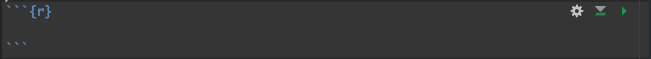
\includegraphics[width=9.04in]{images/3.1codechunk} \caption{RStudio code chunk}\label{fig:unnamed-chunk-14}
\end{figure}

You we can re-run the same operations from before in this code chunk instead of running it in the console. When you are ready, you can click on the green arrow at the top right of the code chunk to execute the entire chunk. The answers will be evaluated in order right beneath the code chunk.

Try

\begin{quote}
Try running the same equations as before but this time in the code chunk. Use the green arrow on the top right of code chunk to evaluate all the equations in the chunk.
\end{quote}

\begin{figure}
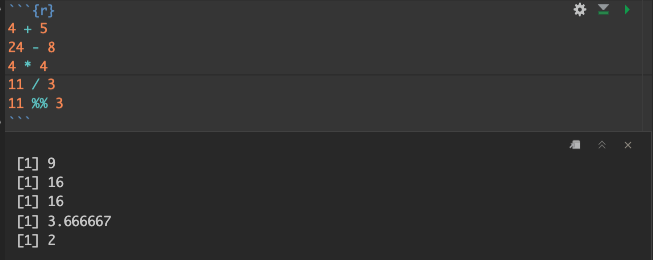
\includegraphics[width=9.07in]{images/3.2codechunkgreen} \caption{RStudio code chunk evaluated}\label{fig:unnamed-chunk-15}
\end{figure}

\hypertarget{storing-variables}{%
\section{Storing Variables}\label{storing-variables}}

We can use the code chunk to help us store variables we might want to reuse later on instead of having to type it out each time.

To assign a value of 8 to the variable \texttt{var1}, you can use the following commands

\begin{quote}
var1 \textless- 4
\end{quote}

or

\begin{quote}
var1 = 4
\end{quote}

Try

\begin{quote}
Create a new code chunk and try storing our previous results to the variables a-e
\end{quote}

\begin{Shaded}
\begin{Highlighting}[]
\NormalTok{a }\OtherTok{\textless{}{-}} \DecValTok{4} \SpecialCharTok{+} \DecValTok{5}
\NormalTok{b }\OtherTok{\textless{}{-}} \DecValTok{24} \SpecialCharTok{{-}} \DecValTok{8}
\NormalTok{c }\OtherTok{\textless{}{-}} \DecValTok{4} \SpecialCharTok{*} \DecValTok{4}
\NormalTok{d }\OtherTok{\textless{}{-}} \DecValTok{11} \SpecialCharTok{/} \DecValTok{3}
\NormalTok{e }\OtherTok{\textless{}{-}} \DecValTok{11} \SpecialCharTok{\%\%} \DecValTok{3}
\end{Highlighting}
\end{Shaded}

\begin{quote}
Note: When you assign a variable, RStudio will store it in the environment panel.
\end{quote}

\begin{figure}
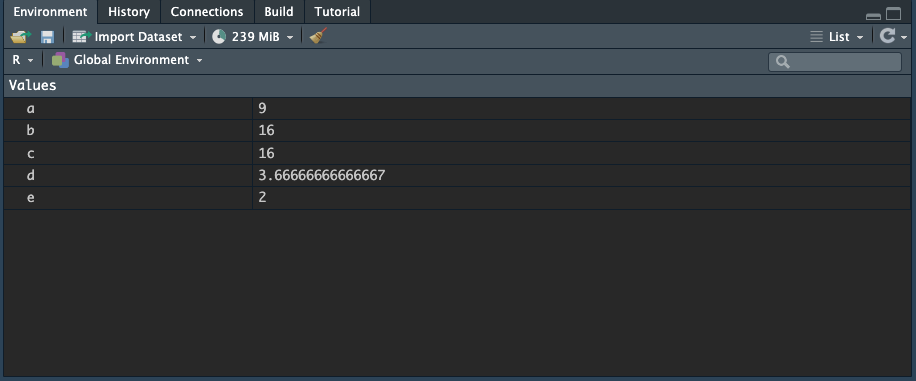
\includegraphics[width=12.72in]{images/3.3variableenvironment} \caption{Updated environemnt}\label{fig:unnamed-chunk-16}
\end{figure}

Once your variable is assigned you can recall the result by calling the variable. We can use the use these variables directly in the console or together in the \emph{R Markdown} file.

Try

\begin{quote}
Try recalling the new variables in both the \textbf{console} and in a \textbf{code chunk}. Create another new code chunk and just type in the variable name. Click on the green arrow when you are ready to evaluate
\end{quote}

\begin{figure}
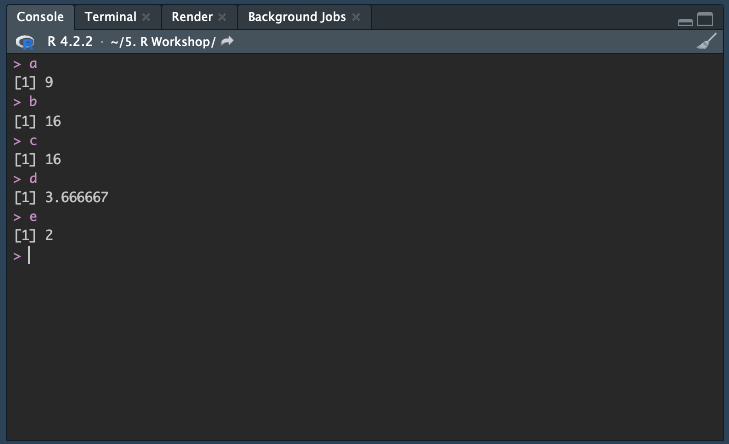
\includegraphics[width=10.12in]{images/3.4variablesconsole} \caption{Using variables console}\label{fig:unnamed-chunk-17}
\end{figure}

\hypertarget{using-variables}{%
\section{Using Variables}\label{using-variables}}

We can also perform the same mathematical operations using stored variables instead of needing to write out.

Try

\begin{quote}
Using a \textbf{code chunk} or just in the \textbf{console}, perform the following operations.
\end{quote}

\begin{Shaded}
\begin{Highlighting}[]
\NormalTok{a }\SpecialCharTok{+}\NormalTok{ a}
\NormalTok{b }\SpecialCharTok{{-}}\NormalTok{ c}
\NormalTok{a }\SpecialCharTok{*}\NormalTok{ d}
\NormalTok{b }\SpecialCharTok{\%\%}\NormalTok{ c}
\end{Highlighting}
\end{Shaded}

\hypertarget{logical-operators}{%
\section{Logical operators}\label{logical-operators}}

\textbf{R} can also perform logical operations as well that include

\begin{itemize}
\item
  Less than: \texttt{\textless{}}
\item
  Less than or equal to: \texttt{\textless{}=}
\item
  Greater than: \texttt{\textgreater{}}
\item
  Greater than or equal to: \texttt{\textgreater{}=}
\item
  Exactly Equal to: \texttt{==}
\item
  Not equal to: \texttt{!=}
\item
  OR: \texttt{\textbar{}}
\item
  AND: \texttt{\&}
\end{itemize}

In any type of programming you do, you will likely run into these logical operations. You will commonly see these types of operators when we are cleaning and preparing data sets for analysis. For health data, we can use logical operators to help us determine disease status or help us separate age groups.

Try

\begin{quote}
Try using the following logical operators on the variables that we created in the \emph{console} or in a \emph{code chunk}
\end{quote}

\begin{Shaded}
\begin{Highlighting}[]
\NormalTok{a }\SpecialCharTok{\textgreater{}}\NormalTok{ b}
\NormalTok{b }\SpecialCharTok{==}\NormalTok{ c}
\NormalTok{e }\SpecialCharTok{\textless{}=}\NormalTok{ b}
\end{Highlighting}
\end{Shaded}

\hypertarget{data-types}{%
\section{Data types}\label{data-types}}

There are different data types you will run into while you are working on a data set including

\begin{itemize}
\item
  \textbf{Numeric}: All real numbers with or without decimals \texttt{8.4}
\item
  \textbf{Integers}: Whole numbers \texttt{29}
\item
  \textbf{Logical}: Boolean values \texttt{TRUE\ or\ FALSE}
\item
  \textbf{Characters}: Characters or String values. A single letter is a character \texttt{A}. A word or a sentence would be a string \texttt{Orange}
\end{itemize}

It is important to know the data type you are working with since some of the common mistakes in cleaning and working with a data set is trying to combine data types that are not compatible.

Try

\begin{quote}
Let's create a new code chunk and create one of each variable time and try to perform some arithmetic operations on them to see what happens.
\end{quote}

Note

\begin{quote}
Logical variables: The proper syntax is all caps TRUE or FALSE
\end{quote}

\begin{quote}
Characters: For strings and characters, you need to surround the word or the letter with single or double quotations. ``Apple'' ``Orange'' `Cat'
\end{quote}

\begin{Shaded}
\begin{Highlighting}[]
\NormalTok{new\_num }\OtherTok{\textless{}{-}} \FloatTok{8.4}

\NormalTok{new\_int }\OtherTok{\textless{}{-}} \DecValTok{29}

\NormalTok{new\_logi }\OtherTok{\textless{}{-}} \ConstantTok{TRUE}

\NormalTok{new\_stringA }\OtherTok{\textless{}{-}} \StringTok{"R Workshop"}

\NormalTok{new\_stringB }\OtherTok{\textless{}{-}} \StringTok{"2023"}
\end{Highlighting}
\end{Shaded}

Note

\begin{quote}
A quick way to check what type of variable you are dealing with is to use the class function. i.e., class(new\_num)
\end{quote}

\begin{Shaded}
\begin{Highlighting}[]
\NormalTok{new\_num }\SpecialCharTok{+}\NormalTok{ new\_int}

\NormalTok{new\_stringA }\SpecialCharTok{==}\NormalTok{ new\_stringB}
\end{Highlighting}
\end{Shaded}

To combine strings together we want to use the \texttt{paste()} function

\begin{Shaded}
\begin{Highlighting}[]
\FunctionTok{paste}\NormalTok{(new\_stringA, new\_stringB)}
\end{Highlighting}
\end{Shaded}

\hypertarget{data-structures}{%
\chapter{Data Structures}\label{data-structures}}

So far we've learned some basics of what you can do in \emph{R} and \emph{R Studio} including the creation and storage of variables. When processing data sets, we need to use data structures for processing, retrieving and storing data. These data structures are

\begin{itemize}
\item
  \textbf{Vectors}: Elements of the same type
\item
  \textbf{Lists}: Contains elements of different types. Can contain store numerical values, strings and characters all together.
\item
  \textbf{Matrices}: arranged in a 2d layout with rows and columns. s
\item
  \textbf{Data frames}: a 2d table-like structure where each column can have a different data type.
\item
  \textbf{Factors}: Used to categorize the data and store it in levels.
\end{itemize}

\hypertarget{vectors}{%
\section{Vectors}\label{vectors}}

This is a one dimensional data structure where all the elements in the vector are the same. Similar to vectors that are found in mathematics.

Imagine you are. Imagine that you're going on a vacation and you need to pack all the essentials in your luggage. To make most space you want to use packing cubes and pack all your similar items together. So all your shirts go in one cube, all your pant in another and, all your electric devices in the third one. You can think of your packing cube as a vector in R, and the items you're packing as the elements of the vector.

\hypertarget{creating-simple-vectors}{%
\subsection{Creating simple vectors}\label{creating-simple-vectors}}

Try

\begin{quote}
Try creating a vector using the \textbf{c( )} function.
\end{quote}

\begin{Shaded}
\begin{Highlighting}[]
\NormalTok{num\_vector }\OtherTok{\textless{}{-}} \FunctionTok{c}\NormalTok{(}\DecValTok{2}\NormalTok{,}\DecValTok{0}\NormalTok{,}\DecValTok{2}\NormalTok{,}\DecValTok{3}\NormalTok{)}

\NormalTok{shirt\_vector }\OtherTok{\textless{}{-}} \FunctionTok{c}\NormalTok{(}\StringTok{"Grey shirt"}\NormalTok{,}\StringTok{"White Shirt"}\NormalTok{,}\StringTok{"Black Shirt"}\NormalTok{)}

\NormalTok{pant\_vector }\OtherTok{\textless{}{-}} \FunctionTok{c}\NormalTok{(}\StringTok{"Blue jeans"}\NormalTok{, }\StringTok{"Beige chinos"}\NormalTok{, }\StringTok{"Black shorts"}\NormalTok{)}

\NormalTok{electronic\_vector }\OtherTok{\textless{}{-}}\FunctionTok{c}\NormalTok{(}\StringTok{"Phone charger"}\NormalTok{, }\StringTok{"Phone cable"}\NormalTok{, }\StringTok{"Laptop"}\NormalTok{)}
\end{Highlighting}
\end{Shaded}

\begin{figure}
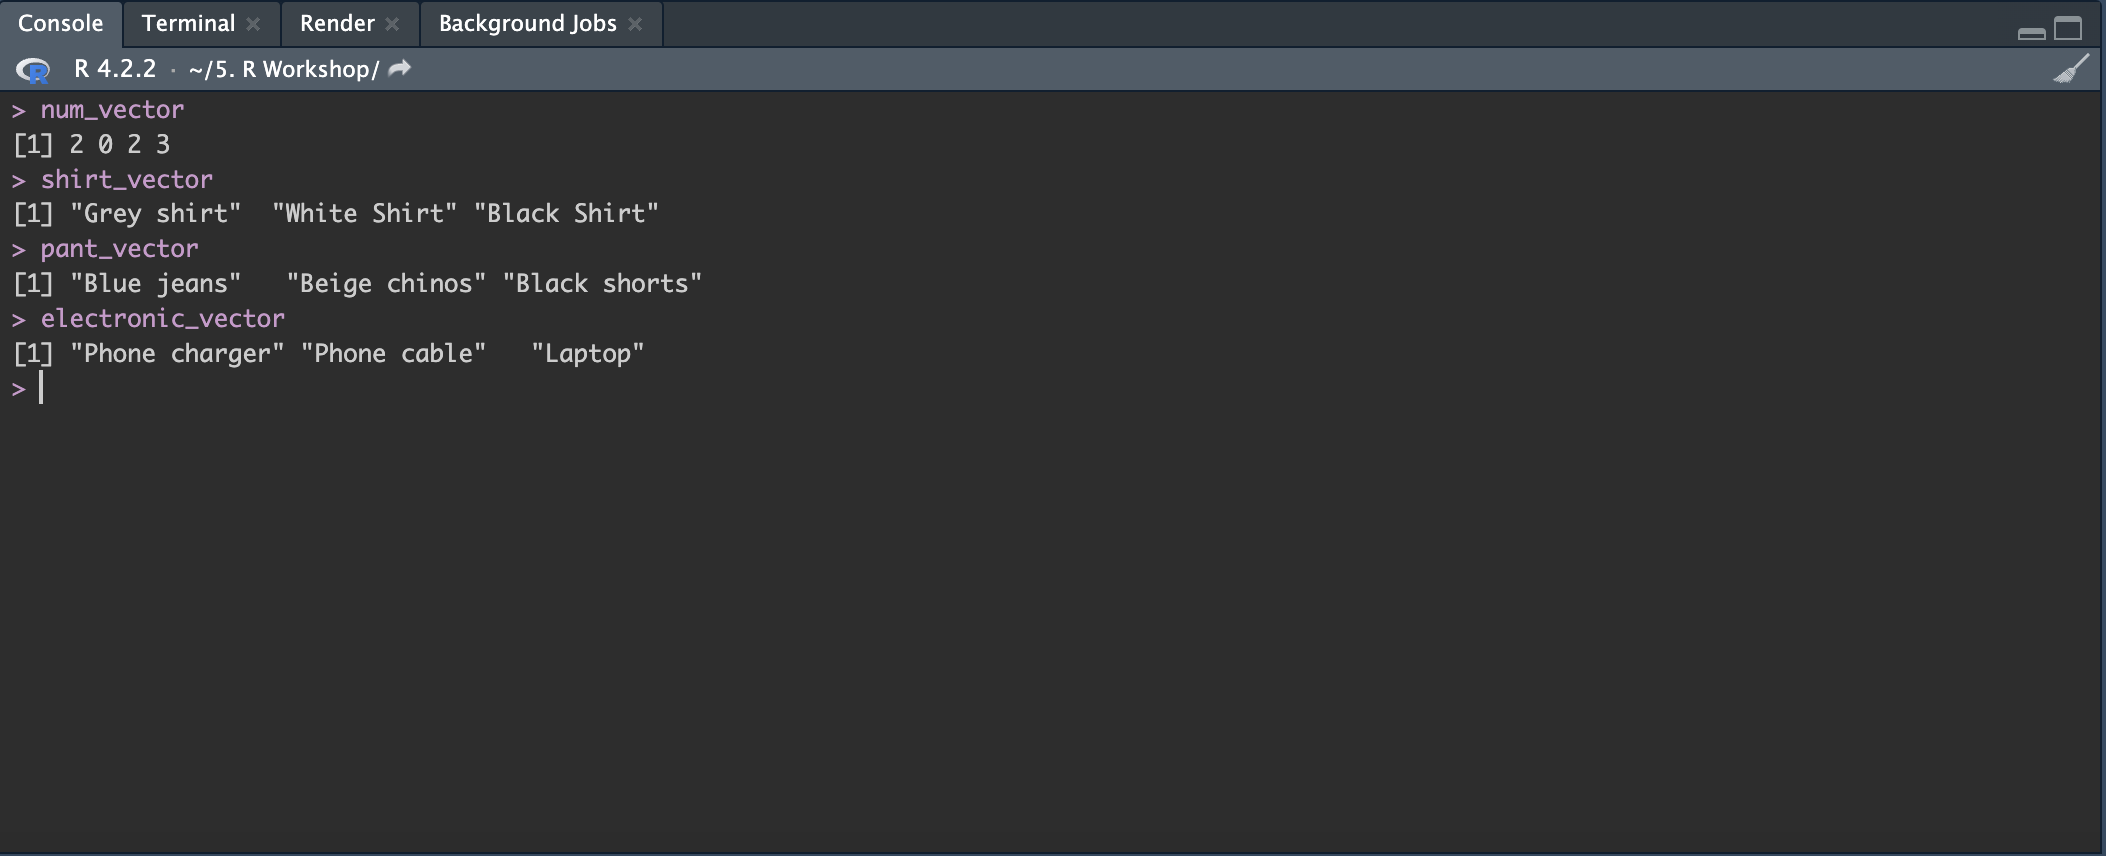
\includegraphics[width=29.25in]{images/3.5vectorconsole} \caption{Basic Vectors}\label{fig:unnamed-chunk-18}
\end{figure}

\hypertarget{simple-vector-operations}{%
\subsection{Simple vector operations}\label{simple-vector-operations}}

One thing that's unique about vectors in R is that you can perform operations on them all at once. Because of your organized packing you are able to double the number of shirts you can pack. If \textbf{num\_vector} represents the number of each shirt, you can simply multiply this by 2 and you can increase the number of shirts you are bringing with you.

Try

\begin{quote}
Try doubling the \textbf{num\_vector} variable you created. Also, try to see what happens when you try to double the \textbf{shirt\_vector}.
\end{quote}

\hypertarget{lists}{%
\section{Lists}\label{lists}}

A list in R is like a container that can hold any type of data. So in this case, your luggage will be a list because it used to hold all the the different items together (shirts, pants, electronics). We will have a luggage list which contains a shirt vector, a pant vector and electronic vector.

\hypertarget{creating-a-list-of-vectors}{%
\subsection{Creating a list of vectors}\label{creating-a-list-of-vectors}}

Try

\begin{quote}
Try to make the luggage list with the our previous vectors by using the \textbf{list( )} function
\end{quote}

\begin{Shaded}
\begin{Highlighting}[]
\NormalTok{luggage\_list }\OtherTok{\textless{}{-}} \FunctionTok{list}\NormalTok{(shirt\_vector, pant\_vector,electronic\_vector)}
\end{Highlighting}
\end{Shaded}

\begin{figure}
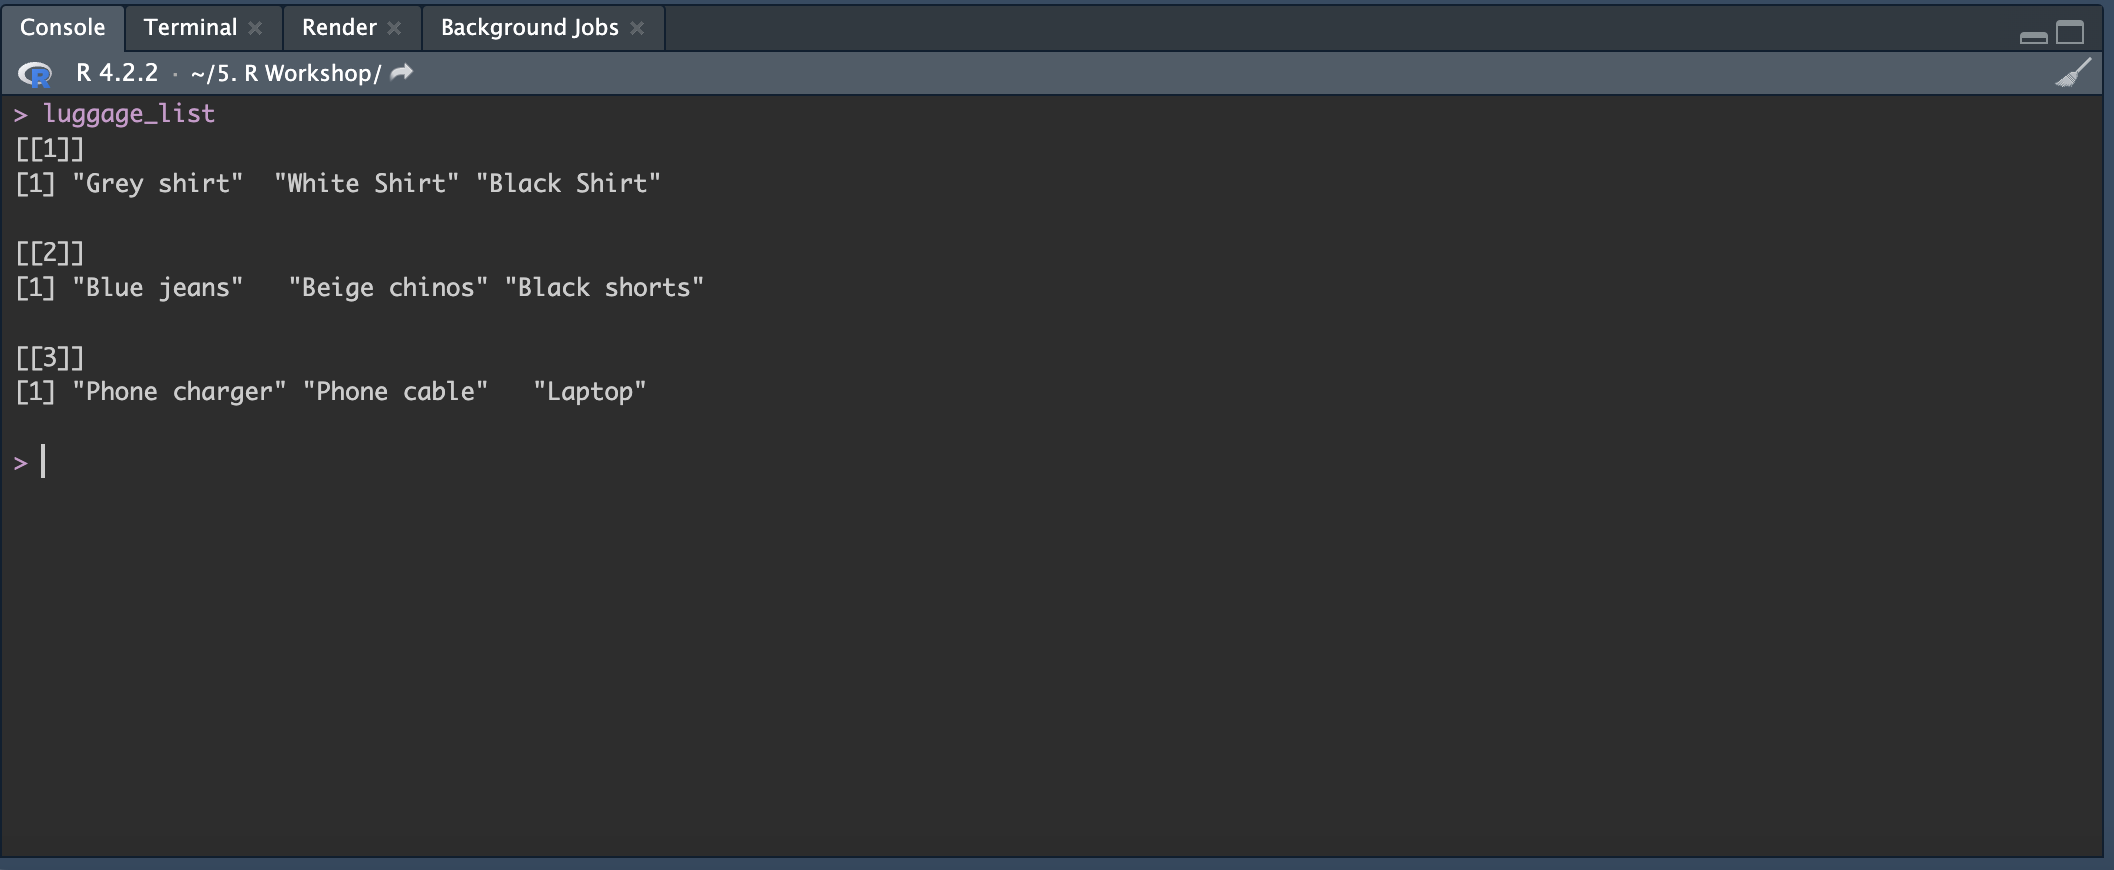
\includegraphics[width=29.36in]{images/3.6listconsole} \caption{Basic Lists}\label{fig:unnamed-chunk-19}
\end{figure}

\hypertarget{accessing-elements-in-the-list}{%
\subsection{Accessing elements in the list}\label{accessing-elements-in-the-list}}

Notice the output we get when we call our list. Our shirts are the first item in our list, pants the second and electronics the third. If you want to check what \textbf{jeans} you packed in your luggage list, you can use \textbf{luggage\_list{[}{[}2{]}{]}}

Try

Try accessing the pants section in our luggage list.

\hypertarget{adding-items-to-lists}{%
\subsection{Adding items to lists}\label{adding-items-to-lists}}

\hypertarget{add-to-the-end}{%
\subsubsection{Add to the end}\label{add-to-the-end}}

Let's say you need to add another packing cube but this time it has all your toiletries. To do this you need try the following:

\begin{Shaded}
\begin{Highlighting}[]
\NormalTok{luggage\_list[[}\FunctionTok{length}\NormalTok{(luggage\_list)}\SpecialCharTok{+}\DecValTok{1}\NormalTok{]] }\OtherTok{\textless{}{-}} \FunctionTok{c}\NormalTok{(}\StringTok{"Toothbrush"}\NormalTok{, }\StringTok{"Toothpaste"}\NormalTok{,}\StringTok{"Floss"}\NormalTok{)}
\end{Highlighting}
\end{Shaded}

If we were to check our list again, we can see that our new toiletry vector has been added to the end of the list.

\hypertarget{add-to-the-front}{%
\subsubsection{Add to the front}\label{add-to-the-front}}

We still have a little bit of space in our luggage and decide to pack some shoes. If we want to add shoes to the front our list try the following

\begin{Shaded}
\begin{Highlighting}[]
\NormalTok{shoes\_vector }\OtherTok{\textless{}{-}} \FunctionTok{c}\NormalTok{(}\StringTok{"Running shoes"}\NormalTok{,}\StringTok{"Sandles"}\NormalTok{)}

\NormalTok{luggage\_list }\OtherTok{\textless{}{-}} \FunctionTok{c}\NormalTok{(}\FunctionTok{list}\NormalTok{(shoes\_vector), luggage\_list)}
\end{Highlighting}
\end{Shaded}

Try

\begin{quote}
Try adding toiletries vector to the end of the list and the shoes vector to the front of our luggage list using the code provided above.
\end{quote}

Your luggage list should now have shoes, shirts, jeans, electronics and toiletries.

\hypertarget{labeling-items-within-lists}{%
\subsection{Labeling items within lists}\label{labeling-items-within-lists}}

Now that our list has grown, we should label each item incase we forget the of our items. To rename the items in the list you can use the \textbf{names( )} function.

\begin{Shaded}
\begin{Highlighting}[]
\FunctionTok{names}\NormalTok{(luggage\_list) }\OtherTok{\textless{}{-}} \FunctionTok{c}\NormalTok{(}\StringTok{"Shoes"}\NormalTok{,}\StringTok{"Shirts"}\NormalTok{,}\StringTok{"Pants"}\NormalTok{,}\StringTok{"Electronics"}\NormalTok{,}\StringTok{"Tolietries"}\NormalTok{)}
\end{Highlighting}
\end{Shaded}

Now we can we can access our items by using the \textbf{\$} symbol which make it easier to check what lists we have.

Try

\begin{quote}
Try accessing the \textbf{Electronics} vector in our luggage\_list using the \textbf{\$} Symbol.
\end{quote}

\begin{figure}
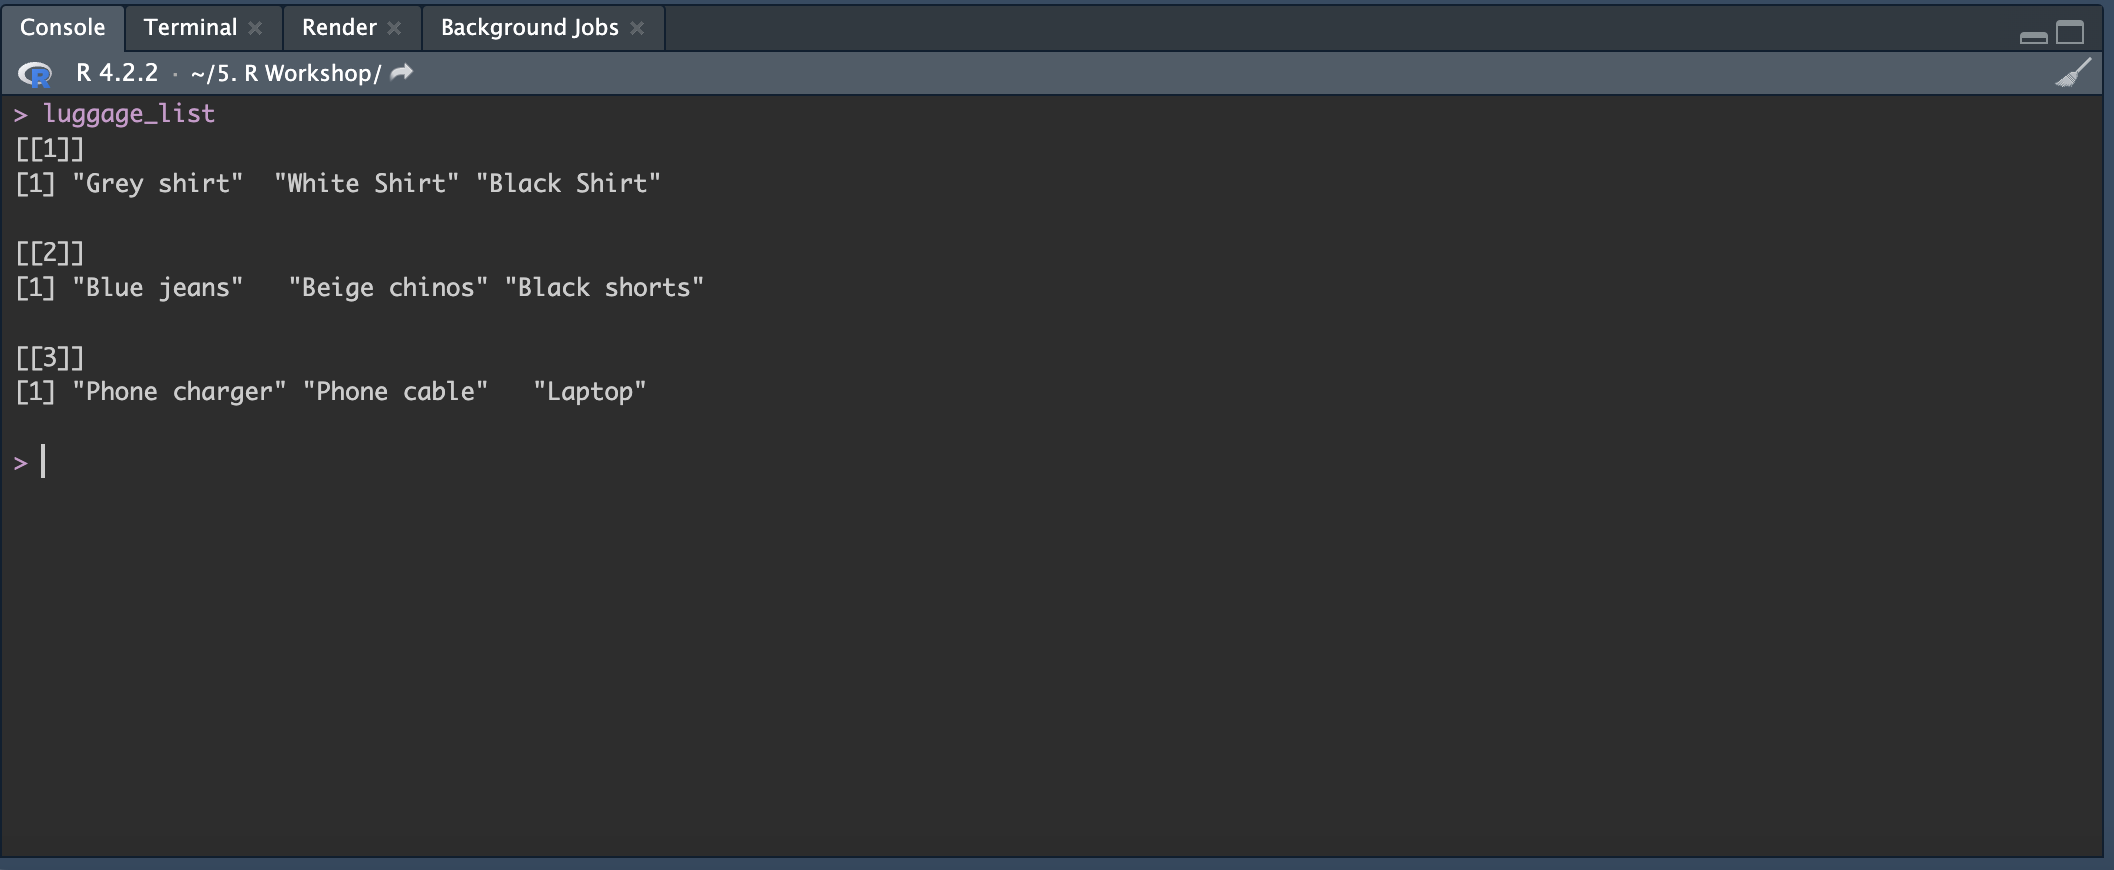
\includegraphics[width=29.36in]{images/3.6listconsole} \caption{Basic Lists}\label{fig:unnamed-chunk-20}
\end{figure}

We have created a \textbf{luggage\_list} that has 5 vectors that are labeled shoes, shirts, pants, electronics and tolietries.

\hypertarget{matrices}{%
\section{Matrices}\label{matrices}}

A matrix 2d data structure that contains rows and columns. Matrices can only contain elements of the same data type, so all the elements in the matrix must be either numeric, character, or logical. Matrices are useful for organizing and manipulating data in a structure and efficient manner since we are able to perform mathematic operations on them, like linear algebra.

In our current example, we can consider a matrix as a packing checklist where each row represents a particular item to pack (such as shirts, pants, or shoes) and each column represents a each of our travel partners luggage. The elements of the matrix could then represent the quantity of each item to pack in each suitcase

\hypertarget{creating-a-matrix}{%
\subsection{Creating a matrix}\label{creating-a-matrix}}

We can generate a matrix using the \textbf{matrix( )} function

\begin{Shaded}
\begin{Highlighting}[]
\NormalTok{packing\_matrix }\OtherTok{\textless{}{-}} \FunctionTok{matrix}\NormalTok{(}\DecValTok{0}\NormalTok{,}\AttributeTok{nrow =} \DecValTok{5}\NormalTok{, }\AttributeTok{ncol=}\DecValTok{3}\NormalTok{)}

\FunctionTok{rownames}\NormalTok{(packing\_matrix) }\OtherTok{\textless{}{-}} \FunctionTok{c}\NormalTok{(}\StringTok{"Shoes"}\NormalTok{, }\StringTok{"Shirts"}\NormalTok{, }\StringTok{"Pants"}\NormalTok{, }\StringTok{"Electronics"}\NormalTok{, }\StringTok{"Toiletries"}\NormalTok{)}

\FunctionTok{colnames}\NormalTok{(packing\_matrix) }\OtherTok{\textless{}{-}} \FunctionTok{c}\NormalTok{(}\StringTok{"My\_Luggage"}\NormalTok{, }\StringTok{"Traveler\_2"}\NormalTok{, }\StringTok{"Travler\_3"}\NormalTok{)}

\FunctionTok{print}\NormalTok{(packing\_matrix)}
\end{Highlighting}
\end{Shaded}

\begin{verbatim}
##             My_Luggage Traveler_2 Travler_3
## Shoes                0          0         0
## Shirts               0          0         0
## Pants                0          0         0
## Electronics          0          0         0
## Toiletries           0          0         0
\end{verbatim}

Try

\begin{quote}
Try creating a packing matrix using the code provided above
\end{quote}

\hypertarget{navigating-the-matrix}{%
\subsection{Navigating the matrix}\label{navigating-the-matrix}}

\hypertarget{filling-in-values}{%
\subsubsection{Filling in values}\label{filling-in-values}}

Now that we have created our matrix, we can access certain columns and rows by indexing which is done using square brackets \emph{{[} {]}}. The synatax for using square brackets would be \textbf{matrix{[}row,column{]}}. Currently, we have no values in our matrix but we can fill them using indexing.

Let's say you ended up packing 2 shoes, 6 shirts, 3 pants, 4 electronics, and 2 toiletries. To add this to your matrix, you would create a vector and then pass that vector into the first column using the indexing syntax

\begin{Shaded}
\begin{Highlighting}[]
\NormalTok{packing\_matrix[, }\DecValTok{1}\NormalTok{] }\OtherTok{\textless{}{-}} \FunctionTok{c}\NormalTok{(}\DecValTok{2}\NormalTok{, }\DecValTok{6}\NormalTok{, }\DecValTok{3}\NormalTok{, }\DecValTok{4}\NormalTok{, }\DecValTok{2}\NormalTok{)}
\end{Highlighting}
\end{Shaded}

Now when check our matrix we should have the first column filled out with the number of items that we packed.

\begin{figure}
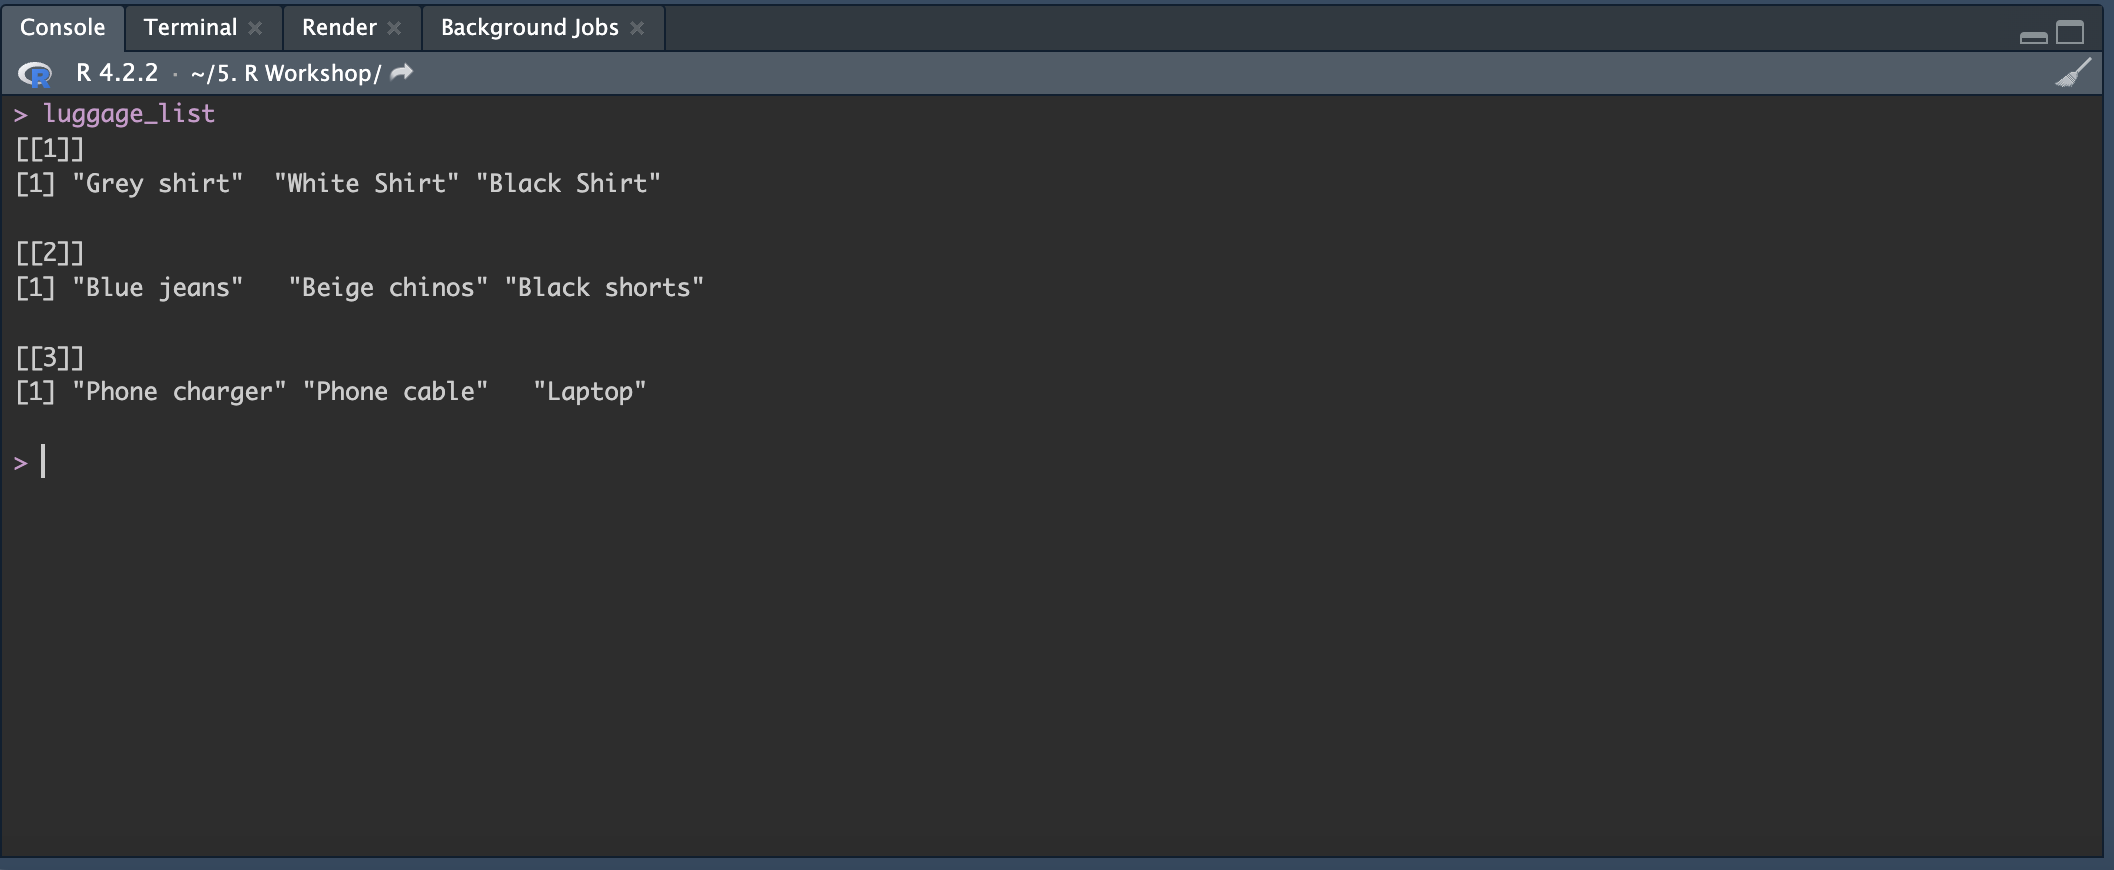
\includegraphics[width=29.36in]{images/3.6listconsole} \caption{Matrix filled}\label{fig:unnamed-chunk-21}
\end{figure}

Try

\begin{quote}
Try filling putting values for Traveler\_2 and Traveler\_3. You can select them yourself or just generate them randomly.
\end{quote}

Note

\begin{quote}
To randomly generate some numbers we can use the sample( ) function.
\end{quote}

\begin{quote}
i.e., sample(1:8, 5, replace = TRUE)
\end{quote}

\begin{Shaded}
\begin{Highlighting}[]
\NormalTok{packing\_matrix[,}\DecValTok{2}\NormalTok{] }\OtherTok{\textless{}{-}} \FunctionTok{sample}\NormalTok{(}\DecValTok{1}\SpecialCharTok{:}\DecValTok{8}\NormalTok{, }\DecValTok{5}\NormalTok{, }\AttributeTok{replace =} \ConstantTok{TRUE}\NormalTok{)}
\NormalTok{packing\_matrix[,}\DecValTok{3}\NormalTok{] }\OtherTok{\textless{}{-}} \FunctionTok{sample}\NormalTok{(}\DecValTok{1}\SpecialCharTok{:}\DecValTok{8}\NormalTok{, }\DecValTok{5}\NormalTok{, }\AttributeTok{replace =} \ConstantTok{TRUE}\NormalTok{)}
\end{Highlighting}
\end{Shaded}

Now that our have filled our packing matrix, we can easily showcase how to access columns and rows in a matrix.

\hypertarget{selecting-columns}{%
\subsubsection{Selecting columns}\label{selecting-columns}}

Let's say we want to double check all the things that were packed for myself. To index a column of a matrix you simply have to use the square brackets. Since we know we are the first column in the matrix we can use \textbf{packing\_matrix{[},1{]}} to find out what we packed.

\begin{Shaded}
\begin{Highlighting}[]
\NormalTok{packing\_matrix[,}\DecValTok{1}\NormalTok{]}
\end{Highlighting}
\end{Shaded}

\begin{verbatim}
##       Shoes      Shirts       Pants Electronics  Toiletries 
##           2           6           3           4           2
\end{verbatim}

Try

\begin{quote}
Try see what Traveler\_2 and Traveler\_3 packed
\end{quote}

\hypertarget{selecting-rows}{%
\subsubsection{Selecting rows}\label{selecting-rows}}

Let's say we are curious on how many shirts each person going on this trip packed. We will still use square brackets, but this time we will be indexing the row instead of the column. \textbf{packing\_matrix{[}1,{]}}

\begin{Shaded}
\begin{Highlighting}[]
\NormalTok{packing\_matrix[}\DecValTok{1}\NormalTok{,]}
\end{Highlighting}
\end{Shaded}

\begin{verbatim}
## My_Luggage Traveler_2  Travler_3 
##          2          4          7
\end{verbatim}

\hypertarget{multiple-selections}{%
\subsubsection{Multiple selections}\label{multiple-selections}}

If we want to see how our packing compares to our travelling partners packing we can use a vector to index 2 columns at the same time.

\begin{Shaded}
\begin{Highlighting}[]
\NormalTok{packing\_matrix[,}\FunctionTok{c}\NormalTok{(}\DecValTok{1}\NormalTok{,}\DecValTok{3}\NormalTok{)]}
\end{Highlighting}
\end{Shaded}

\begin{verbatim}
##             My_Luggage Travler_3
## Shoes                2         7
## Shirts               6         8
## Pants                3         2
## Electronics          4         8
## Toiletries           2         4
\end{verbatim}

We can also index a certain range instead of selecting specific rows or columns. Let's say we want to check the what each person packed for shoes, shirts and pants. We could index using a vector by putting all 3 numbers or we can use a colon \emph{:} to check the range.

\begin{Shaded}
\begin{Highlighting}[]
\NormalTok{packing\_matrix[}\DecValTok{1}\SpecialCharTok{:}\DecValTok{3}\NormalTok{,]}
\end{Highlighting}
\end{Shaded}

\begin{verbatim}
##        My_Luggage Traveler_2 Travler_3
## Shoes           2          4         7
## Shirts          6          8         8
## Pants           3          7         2
\end{verbatim}

\hypertarget{dataframes}{%
\section{Dataframes}\label{dataframes}}

Dataframes is a very popular data structure in R since they are easy to work with and allows you do organize and work with data very effciently. A dataframe is another tabular object like the matrix but the difference between the two is that you can store different types of data in a dataframe. Think of it simliar to an excel spreadsheet where you can different types of data for each column (age, gender, income, etc.).

\hypertarget{creating-a-dataframe}{%
\subsection{Creating a dataframe}\label{creating-a-dataframe}}

So with our vacation example, we can use a dataframe to keep track of the preferences of each traveler with the following variables.

\begin{itemize}
\item
  Age (numerical)
\item
  Gender (factor)
\item
  Budget (numerical)
\item
  Number of luggages (numerical)
\item
  Weight of luggages (numerical)
\item
  Food allergies (string)
\item
  Activities (string)
\item
  Must see places (string)
\end{itemize}

Note

\begin{quote}
To create a dataframe you can use the function \textbf{data.frame( )}
\end{quote}

\begin{Shaded}
\begin{Highlighting}[]
\NormalTok{travelers }\OtherTok{\textless{}{-}} \FunctionTok{data.frame}\NormalTok{(}
  \AttributeTok{Age =} \FunctionTok{c}\NormalTok{(}\DecValTok{25}\NormalTok{, }\DecValTok{30}\NormalTok{, }\DecValTok{35}\NormalTok{),}
  \AttributeTok{Gender =} \FunctionTok{factor}\NormalTok{(}\FunctionTok{c}\NormalTok{(}\StringTok{"Female"}\NormalTok{, }\StringTok{"Male"}\NormalTok{, }\StringTok{"Non{-}binary"}\NormalTok{), }\AttributeTok{levels =} \FunctionTok{c}\NormalTok{(}\StringTok{"Male"}\NormalTok{, }\StringTok{"Female"}\NormalTok{, }\StringTok{"Non{-}binary"}\NormalTok{)),}
  \AttributeTok{Budget =} \FunctionTok{c}\NormalTok{(}\DecValTok{1500}\NormalTok{, }\DecValTok{2500}\NormalTok{, }\DecValTok{2000}\NormalTok{),}
  \AttributeTok{Num\_luggages =} \FunctionTok{c}\NormalTok{(}\DecValTok{2}\NormalTok{, }\DecValTok{3}\NormalTok{, }\DecValTok{1}\NormalTok{),}
  \AttributeTok{Weight\_luggages =} \FunctionTok{c}\NormalTok{(}\DecValTok{20}\NormalTok{, }\DecValTok{15}\NormalTok{, }\DecValTok{25}\NormalTok{),}
  \AttributeTok{Food\_allergies =} \FunctionTok{c}\NormalTok{(}\StringTok{"Peanuts, shellfish"}\NormalTok{, }\StringTok{"Gluten, dairy"}\NormalTok{, }\StringTok{"None"}\NormalTok{),}
  \AttributeTok{Activities =} \FunctionTok{c}\NormalTok{(}\StringTok{"Hiking, sightseeing"}\NormalTok{, }\StringTok{"Museums, beach"}\NormalTok{, }\StringTok{"Shopping, nightlife"}\NormalTok{),}
  \AttributeTok{Must\_see\_places =} \FunctionTok{c}\NormalTok{(}\StringTok{"Eiffel Tower, Colosseum"}\NormalTok{, }\StringTok{"Statue of Liberty, Grand Canyon"}\NormalTok{, }\StringTok{"Golden Gate Bridge, Machu Picchu"}\NormalTok{)}
\NormalTok{)}

\FunctionTok{print}\NormalTok{(travelers)}
\end{Highlighting}
\end{Shaded}

\begin{verbatim}
##   Age     Gender Budget Num_luggages Weight_luggages     Food_allergies
## 1  25     Female   1500            2              20 Peanuts, shellfish
## 2  30       Male   2500            3              15      Gluten, dairy
## 3  35 Non-binary   2000            1              25               None
##            Activities                  Must_see_places
## 1 Hiking, sightseeing          Eiffel Tower, Colosseum
## 2      Museums, beach  Statue of Liberty, Grand Canyon
## 3 Shopping, nightlife Golden Gate Bridge, Machu Picchu
\end{verbatim}

\hypertarget{using-the-a-dataframe}{%
\subsection{Using the a dataframe}\label{using-the-a-dataframe}}

\hypertarget{manipulating-data}{%
\subsubsection{Manipulating data}\label{manipulating-data}}

Like spreedsheets, we can manipulate the dataframe to create new variables. If we wanted to find out the average weight of the luggages we can use build in mean function

\begin{Shaded}
\begin{Highlighting}[]
\FunctionTok{mean}\NormalTok{(travelers}\SpecialCharTok{$}\NormalTok{Weight\_luggages)}
\end{Highlighting}
\end{Shaded}

\begin{verbatim}
## [1] 20
\end{verbatim}

We can also find the median as well using the median function

\begin{Shaded}
\begin{Highlighting}[]
\FunctionTok{median}\NormalTok{(travelers}\SpecialCharTok{$}\NormalTok{Weight\_luggages)}
\end{Highlighting}
\end{Shaded}

\begin{verbatim}
## [1] 20
\end{verbatim}

\hypertarget{subsetting-data}{%
\subsubsection{Subsetting data}\label{subsetting-data}}

If we don't want all the columns, we can subset what we need into a new dataframe using square brackets \textbf{df{[}row,col{]}}. If we wanted to to look \textbf{Age}, \textbf{Gender} and, \textbf{Budget} we can use the following code.

Note:

\begin{quote}
This is using base R, we will be using a package later on called `dplyr' to also subset the data
\end{quote}

\begin{Shaded}
\begin{Highlighting}[]
\NormalTok{travelers[,}\DecValTok{1}\SpecialCharTok{:}\DecValTok{3}\NormalTok{]}
\end{Highlighting}
\end{Shaded}

\begin{verbatim}
##   Age     Gender Budget
## 1  25     Female   1500
## 2  30       Male   2500
## 3  35 Non-binary   2000
\end{verbatim}

Note:

\begin{quote}
If we didn't know the names the columns we can use the \textbf{names( )} function to find out the column names.
\end{quote}

\begin{quote}
If we knew the names, we can also subset using a vector and the names of the columns we want to subset \textbf{travelers{[},c(``Age'',``Gender'',``Budget''){]}}
\end{quote}

\hypertarget{filtering-data}{%
\subsubsection{Filtering data}\label{filtering-data}}

Let's say that we are only interested in those who have a budget that is \textbf{\textless{} 2500}. We can use the logical statements that were introduced in Chapter 3 to do this.

\begin{Shaded}
\begin{Highlighting}[]
\NormalTok{travelers[travelers}\SpecialCharTok{$}\NormalTok{Budget }\SpecialCharTok{\textless{}}\DecValTok{2500}\NormalTok{, ]}
\end{Highlighting}
\end{Shaded}

\begin{verbatim}
##   Age     Gender Budget Num_luggages Weight_luggages     Food_allergies
## 1  25     Female   1500            2              20 Peanuts, shellfish
## 3  35 Non-binary   2000            1              25               None
##            Activities                  Must_see_places
## 1 Hiking, sightseeing          Eiffel Tower, Colosseum
## 3 Shopping, nightlife Golden Gate Bridge, Machu Picchu
\end{verbatim}

Try

\begin{quote}
Try to subset the dataframe for \textbf{Age \textgreater{} 25}
\end{quote}

\begin{Shaded}
\begin{Highlighting}[]
\NormalTok{travelers[travelers}\SpecialCharTok{$}\NormalTok{Age }\SpecialCharTok{\textgreater{}}\DecValTok{25}\NormalTok{, ]}
\end{Highlighting}
\end{Shaded}

\begin{verbatim}
##   Age     Gender Budget Num_luggages Weight_luggages Food_allergies
## 2  30       Male   2500            3              15  Gluten, dairy
## 3  35 Non-binary   2000            1              25           None
##            Activities                  Must_see_places
## 2      Museums, beach  Statue of Liberty, Grand Canyon
## 3 Shopping, nightlife Golden Gate Bridge, Machu Picchu
\end{verbatim}

\hypertarget{factors}{%
\section{Factors}\label{factors}}

Factors are used to represent categorical variables such as \textbf{Gender} or \textbf{Income levels}. Using the \emph{factor( )} function, we can change text data types to factor data types and use built in-functions to work with categorical data.

You may have noticed before when we created our travel dataframe that gender was coded using the \emph{factor( )}

\begin{Shaded}
\begin{Highlighting}[]
\FunctionTok{factor}\NormalTok{(}\FunctionTok{c}\NormalTok{(}\StringTok{"Female"}\NormalTok{, }\StringTok{"Male"}\NormalTok{, }\StringTok{"Non{-}binary"}\NormalTok{), }\AttributeTok{levels =} \FunctionTok{c}\NormalTok{(}\StringTok{"Male"}\NormalTok{, }\StringTok{"Female"}\NormalTok{, }\StringTok{"Non{-}binary"}\NormalTok{))}
\end{Highlighting}
\end{Shaded}

\begin{verbatim}
## [1] Female     Male       Non-binary
## Levels: Male Female Non-binary
\end{verbatim}

we can use the table function to show us the number observations in each category.

\begin{Shaded}
\begin{Highlighting}[]
\FunctionTok{table}\NormalTok{(travelers}\SpecialCharTok{$}\NormalTok{Gender)}
\end{Highlighting}
\end{Shaded}

\begin{verbatim}
## 
##       Male     Female Non-binary 
##          1          1          1
\end{verbatim}

the \emph{levels( )} function will show the order of our categorical variable. In our \textbf{travelers} dataframe, we set the levels as \textbf{Male, Female, Non-binary}. If want to know the integer representation we can use the \textbf{as.numeric( )} function to show us the order. In our example, the first traveler is \textbf{``Female''}, second is \textbf{``Male''} and, third is \textbf{``Non-binary''}.

\begin{Shaded}
\begin{Highlighting}[]
\FunctionTok{as.numeric}\NormalTok{(travelers}\SpecialCharTok{$}\NormalTok{Gender)}
\end{Highlighting}
\end{Shaded}

\begin{verbatim}
## [1] 2 1 3
\end{verbatim}

\hypertarget{data-wrangling}{%
\chapter{Data Wrangling}\label{data-wrangling}}

\hypertarget{r-packages}{%
\section{R Packages}\label{r-packages}}

Packages are a collection of functions that extend the functionality of R. They are tools that help with data analysis, modelling, data visualization. Some of the most common packages in R is \textbf{ggplot2} for data visualization, \textbf{dplyr} for data wrangling/manipulation and \emph{caret} for machine learning.

\hypertarget{installing-packages}{%
\subsection{Installing Packages}\label{installing-packages}}

To use packages we will have the the \textbf{install.packages( )} function and put in the package. We can either does this as a \emph{chunk} in a R-markdown file or we can type it directly into the console.

Try

\begin{quote}
Try installing \textbf{dplyr} and \textbf{ggplot2} packages
\end{quote}

Note

\begin{quote}
You can install multiple packages are the same time if you put then in a vector and before using the \textbf{install.packages( )} function.
\end{quote}

\begin{quote}
i.e., install.packages(c(`dplyr',`ggplot2'))
\end{quote}

\hypertarget{using-packages}{%
\subsection{Using Packages}\label{using-packages}}

\hypertarget{loading-packages}{%
\subsubsection{Loading Packages}\label{loading-packages}}

After installing our packages, we have to load them using the \textbf{library( )} function or the \textbf{require( )} function. This is similar to opening up a new app or program that you just installed.

\begin{Shaded}
\begin{Highlighting}[]
\FunctionTok{library}\NormalTok{(dplyr)}
\end{Highlighting}
\end{Shaded}

\begin{verbatim}
## 
## Attaching package: 'dplyr'
\end{verbatim}

\begin{verbatim}
## The following objects are masked from 'package:stats':
## 
##     filter, lag
\end{verbatim}

\begin{verbatim}
## The following objects are masked from 'package:base':
## 
##     intersect, setdiff, setequal, union
\end{verbatim}

\hypertarget{dplyr}{%
\section{dplyr}\label{dplyr}}

The \textbf{dplyr} is used for data manipulation and can allow us to work with data more efficiently than with base R. We can do the same operations in our previous \emph{travelers} dataframe using \textbf{dplyr}.

\hypertarget{pipe-function}{%
\subsection{Pipe function (\%\textgreater\%)}\label{pipe-function}}

This is one of the most powerful functions in the \textbf{dplyr} package. What the pipe function does is takes the output of one function and then passes it along to the next one. So instead of saving results to multiple variables, we can perform a sequence of commands in as one command. Using our previous \textbf{travelers} dataframe, we were able to calculate the \emph{mean luggage weight} for all travelers but what if we are interested in the total weight of the luggage each traveler is bringing? We can do this in \textbf{dplyr} using the pipe function (\%\textgreater\%) and \textbf{mutate( )} function, which creates a new column. We can also subset the data as in the same function as well. Let's say we are only interested in all the numerical values, we can use the \textbf{select} function to ask it to select all the columns that hold numerical data.

\begin{Shaded}
\begin{Highlighting}[]
\NormalTok{travelers }\SpecialCharTok{\%\textgreater{}\%}
  \FunctionTok{mutate}\NormalTok{(}\AttributeTok{mean\_weight =}\NormalTok{ Weight\_luggages}\SpecialCharTok{/}\NormalTok{Num\_luggages) }\SpecialCharTok{\%\textgreater{}\%}
  \FunctionTok{select}\NormalTok{(}\FunctionTok{c}\NormalTok{(}\FunctionTok{where}\NormalTok{(is.numeric)))}
\end{Highlighting}
\end{Shaded}

\begin{verbatim}
##   Age Budget Num_luggages Weight_luggages mean_weight
## 1  25   1500            2              20          10
## 2  30   2500            3              15           5
## 3  35   2000            1              25          25
\end{verbatim}

You can see our new column \textbf{mean\_weight} added to the end and that the dataframe only contains numerical values. If we were to do this without the pipe function, we would first need to get add the \textbf{mean\_weight} column, save it, then subset our data for all numeric values including our new column.

Lets say we want to filter our data finding travelers with a \textbf{age \textgreater25} or if they have a \textbf{budget \textgreater2500}. We can do this all together in one command using dplyr using the \textbf{filter( )} command.

\begin{Shaded}
\begin{Highlighting}[]
\NormalTok{travelers }\SpecialCharTok{\%\textgreater{}\%} 
  \FunctionTok{filter}\NormalTok{(Age }\SpecialCharTok{\textgreater{}} \DecValTok{25} \SpecialCharTok{|}\NormalTok{ Budget }\SpecialCharTok{\textgreater{}} \DecValTok{2500}\NormalTok{)}
\end{Highlighting}
\end{Shaded}

\begin{verbatim}
##   Age     Gender Budget Num_luggages Weight_luggages Food_allergies
## 1  30       Male   2500            3              15  Gluten, dairy
## 2  35 Non-binary   2000            1              25           None
##            Activities                  Must_see_places
## 1      Museums, beach  Statue of Liberty, Grand Canyon
## 2 Shopping, nightlife Golden Gate Bridge, Machu Picchu
\end{verbatim}

Note

\begin{quote}
The \emph{\textbar{}} is the logical statment \textbf{OR} in R. \emph{\&} is the logical statment for \textbf{AND}
\end{quote}

We can see that we have 2 entries that are either \textbf{Age \textgreater25} or have a \textbf{Budget \textgreater2500}

There are a lot more functions that are part of dplyr package. The most common ones for data manipulation are

\begin{itemize}
\item
  mutate() - Adds a new variable to your dataframe based on existing variables
\item
  select() - Picks variables from a dataframe based on their names
\item
  filter() - Picks out cases based on criteria
\item
  summarise() - Reduces down values down to a single summary
\item
  arrange() - Changes the order of the rows based
\end{itemize}

For more information or more practice you can go to the dplyr website which also has a R-bookdown on data transformation.

\url{https://dplyr.tidyverse.org/}

\hypertarget{loading-datasets}{%
\section{Loading datasets}\label{loading-datasets}}

More often than not, we will be working with a datasets instead of creating our own. In \textbf{R} we can load the different types of files, the most common being a comma separated file (\textbf{CSV}). Now that we have our travelers preferences and budget we need to find a destination that would be suitable for each of our travelers. We will be using a few datasets from \textbf{Numbeo.com} and \textbf{The World bank}.

We want to save these as variables so we can access them later.

To load a dataset, we will use the \textbf{read.csv( )} function and save the dataset as a variable in our environment. The first one we want to load is from \textbf{numbeo.com} which shows us the cost of a inexpensive meal at a restaurant.

Note

\begin{quote}
The data from \textbf{numbeo.com} is aggregated by user submissions and calculates the average costs of certain products
\end{quote}

\begin{Shaded}
\begin{Highlighting}[]
\NormalTok{meals }\OtherTok{\textless{}{-}} \FunctionTok{read.csv}\NormalTok{(}\StringTok{"data/numbeo\_meal.csv"}\NormalTok{)}
\end{Highlighting}
\end{Shaded}

Another way to load your data is using the import function in R studio.

When you select the file you want to import a window will appear and you can do some quick modification to our data if needed.

Note

\begin{quote}
One of the most common issues when using this feature is the setting the headers. There is a radial button for the header which you can toggle on and off.
\end{quote}

Try

\begin{quote}
We will be making use of the ticket, arrivals and, country codes dataset. You can try loading these files with the interface or using a code chunk.
\end{quote}

\begin{Shaded}
\begin{Highlighting}[]
\NormalTok{ticket }\OtherTok{\textless{}{-}} \FunctionTok{read.csv}\NormalTok{(}\StringTok{"data/numbeo\_ticket.csv"}\NormalTok{)}
\NormalTok{arrival }\OtherTok{\textless{}{-}} \FunctionTok{read.csv}\NormalTok{(}\StringTok{"data/world\_bank\_arrival.csv"}\NormalTok{)}
\NormalTok{country\_codes }\OtherTok{\textless{}{-}} \FunctionTok{read.csv}\NormalTok{(}\StringTok{"data/country\_codes\_iso.csv"}\NormalTok{)}
\end{Highlighting}
\end{Shaded}

\hypertarget{understanding-your-dataset}{%
\section{Understanding your dataset}\label{understanding-your-dataset}}

Understanding your datasets is important when performing data analysis. The more familiar you are with the shape of your dataset, the more insights you are able to pull out from it. This includes knowing the number of rows and columns as well as the types of columns that you are working with.

We can use the \textbf{View( )} function in order to open up a new tab to view the dataset like an excel sheet.

Note

\begin{quote}
This function is case sensitive and must be called with a uppercase \textbf{V}
\end{quote}

\begin{Shaded}
\begin{Highlighting}[]
\FunctionTok{View}\NormalTok{(meals)}
\end{Highlighting}
\end{Shaded}

To quickly look at the first 6 rows of the data we can use the \textbf{head( )} function.

\begin{Shaded}
\begin{Highlighting}[]
\FunctionTok{head}\NormalTok{(meals,}\DecValTok{3}\NormalTok{)}
\end{Highlighting}
\end{Shaded}

\begin{verbatim}
##         Country Meal_Inexpensive_Restaurant
## 1   Switzerland                       37.35
## 2       Denmark                       27.58
## 3 United States                       26.72
\end{verbatim}

Note

\begin{quote}
You can specify the number of rows you want to examine by adding the number to function
\end{quote}

\begin{quote}
i.e., \textbf{head(meals,4)}
\end{quote}

You can also view the last rows of the column using the \textbf{tail( )} function

\begin{Shaded}
\begin{Highlighting}[]
\FunctionTok{tail}\NormalTok{(meals,}\DecValTok{3}\NormalTok{)}
\end{Highlighting}
\end{Shaded}

\begin{verbatim}
##       Country Meal_Inexpensive_Restaurant
## 103 Sri Lanka                        2.05
## 104   Nigeria                        2.02
## 105  Pakistan                        1.65
\end{verbatim}

We can do some quick summary statistics using the \textbf{summary( )} function as well. Depending on the type of data in each column, we can see the length or a number summary including the min, max, mean, median, mode, and the 1st and 3rd quartiles.

\begin{Shaded}
\begin{Highlighting}[]
\FunctionTok{summary}\NormalTok{(meals)}
\end{Highlighting}
\end{Shaded}

\begin{verbatim}
##    Country          Meal_Inexpensive_Restaurant
##  Length:105         Min.   : 1.65              
##  Class :character   1st Qu.: 5.87              
##  Mode  :character   Median :10.21              
##                     Mean   :11.53              
##                     3rd Qu.:15.52              
##                     Max.   :37.35
\end{verbatim}

\hypertarget{combining-your-dataset}{%
\section{Combining your dataset}\label{combining-your-dataset}}

Currently we have 4 separate datasets that contain all the information we need. Our goal is to combine all the dataset to a singular one which we can start our data analysis. To do this need something that is unique for all the entries. In our case, the ISO country code and the country name are something that is unique for each entry.

We will be using the country\_codes dataset as our base.

\hypertarget{binds}{%
\subsection{Binds}\label{binds}}

There are different types of ways to join your dataset depending on your desired outcome. Sometimes we just need to add columns or rows to the base dataset. For this, we can use either \textbf{rbind( )} or \textbf{cbind( )} if the conditions are appropriate.

\begin{itemize}
\item
  rbind() - row bind will add rows to the base dataset if they number of rows and the row names are the same.
\item
  cbind() - column bind will add more columns to the base dataset if the they have the same number of rows.
\end{itemize}

\hypertarget{joins}{%
\subsection{Joins}\label{joins}}

Most times, we will have an unequal amount of rows or columns and we want to match with something unique to eaach row. For this we can utilize joins. There are different types of joins you can use that all perform their task differently.

\begin{itemize}
\item
  left\_join() - Matches all paired variables to the left dataframe
\item
  right\_join() - Matches all paired variables to the right dataframe
\item
  inner\_join() - Returns a dataframe with only matching variables. If their is no matching variable, it does not get included.
\item
  full\_join() - Keeps all variables from both dataframes even if they do not match.
\end{itemize}

Note

\begin{quote}
left\_join() is the most common join you will be using during a data analysis
\end{quote}

Let's try to combine all 4 datasets into one working dataset. First we want to combine our \emph{meal} and \emph{ticket} dataframes since they have the same number of rows. We will use a \emph{left\_join( )} to combine these based on the country name.

Try

\begin{quote}
Try to perform a \emph{left\_join( )} on the \emph{meal} and \emph{ticket} based on \emph{Country} name.
\end{quote}

\begin{Shaded}
\begin{Highlighting}[]
\NormalTok{travel\_meal\_tickets }\OtherTok{\textless{}{-}} \FunctionTok{left\_join}\NormalTok{(meals,ticket,}\AttributeTok{by =} \StringTok{"Country"}\NormalTok{)}
\FunctionTok{head}\NormalTok{(travel\_meal\_tickets,}\DecValTok{3}\NormalTok{)}
\end{Highlighting}
\end{Shaded}

\begin{verbatim}
##         Country Meal_Inexpensive_Restaurant one_way_ticket_local
## 1   Switzerland                       37.35                 5.38
## 2       Denmark                       27.58                 4.73
## 3 United States                       26.72                 3.34
\end{verbatim}

Using a left join, we now have a single dataframe with 3 columns, Country name, the price for the restaurants and price for a one way ticket.

Next, lets combine this dataframe with the country codes dataframe. Looking at the \textbf{country code} dataframe, we have 4 columns and 249 rows. We do need some cleaning on this dataframe before continuing. Let's keep the Country column and just the 3 digit alpha code using \textbf{dplyr} and the \textbf{select( )} function

\begin{Shaded}
\begin{Highlighting}[]
\NormalTok{country\_code\_subset }\OtherTok{\textless{}{-}}\NormalTok{ country\_codes }\SpecialCharTok{\%\textgreater{}\%}
  \FunctionTok{select}\NormalTok{(}\FunctionTok{c}\NormalTok{(Country,alpha\_3\_code)) }\SpecialCharTok{\%\textgreater{}\%}
  \FunctionTok{rename}\NormalTok{(}\AttributeTok{country\_code =}\NormalTok{ alpha\_3\_code)}

\FunctionTok{head}\NormalTok{(country\_code\_subset,}\DecValTok{3}\NormalTok{)}
\end{Highlighting}
\end{Shaded}

\begin{verbatim}
##       Country country_code
## 1 Afghanistan          AFG
## 2     Albania          ALB
## 3     Algeria          DZA
\end{verbatim}

We want to use our new subset of the country\_codes as our base model and join the meal/ticket dataframe to this one. Since the country code has 249 rows and the meal/ticket one has 105 rows. We want to use a full join here because we aren't sure of the country names are spelled the same in each dataframes. Using the \textbf{filter( )} function, we can filter out which alpha\_3\_codes are missing and we notice there is just one which is Kosovo.

\begin{Shaded}
\begin{Highlighting}[]
\NormalTok{country\_ticket\_meal\_code }\OtherTok{\textless{}{-}} \FunctionTok{full\_join}\NormalTok{(country\_code\_subset,travel\_meal\_tickets, }\AttributeTok{by =} \StringTok{"Country"}\NormalTok{)}

\FunctionTok{head}\NormalTok{(country\_ticket\_meal\_code,}\DecValTok{3}\NormalTok{)}
\end{Highlighting}
\end{Shaded}

\begin{verbatim}
##       Country country_code Meal_Inexpensive_Restaurant one_way_ticket_local
## 1 Afghanistan          AFG                          NA                   NA
## 2     Albania          ALB                        7.79                 0.52
## 3     Algeria          DZA                        2.96                 0.25
\end{verbatim}

Using the \textbf{filter( )} function, we can filter out which alpha\_3\_codes are missing and we notice there is just one which is Kosovo.

Note

\begin{quote}
Kosovo is not country recognized by ISO 3166 standards.
\end{quote}

Finally we want to join our last database which is the from the world bank that contains the number of arrivals to the country from 1960 - 2021 however, we need to perform some data cleaning before we can combine them together. Having a look at our dataframe we see each columns for years has a \textbf{\emph{X}} in front of it. We will want to rename that by using the \textbf{rename\_all( )} which is part of the \textbf{dplyr} package.

Note

\begin{quote}
The period \textbf{(.)} being used here is a special character here that means for this ``For this current dataframe''
\end{quote}

\begin{Shaded}
\begin{Highlighting}[]
\NormalTok{arrival\_clean }\OtherTok{\textless{}{-}}\NormalTok{ arrival }\SpecialCharTok{\%\textgreater{}\%} 
  \FunctionTok{rename\_all}\NormalTok{(}\SpecialCharTok{\textasciitilde{}}\NormalTok{stringr}\SpecialCharTok{::}\FunctionTok{str\_replace}\NormalTok{(.,}\StringTok{"\^{}X"}\NormalTok{,}\StringTok{""}\NormalTok{))}

\FunctionTok{head}\NormalTok{(arrival,}\DecValTok{3}\NormalTok{)}
\end{Highlighting}
\end{Shaded}

\begin{verbatim}
##                       Country country_code X1960 X1961 X1962 X1963 X1964 X1965
## 1                       Aruba          ABW    NA    NA    NA    NA    NA    NA
## 2 Africa Eastern and Southern          AFE    NA    NA    NA    NA    NA    NA
## 3                 Afghanistan          AFG    NA    NA    NA    NA    NA    NA
##   X1966 X1967 X1968 X1969 X1970 X1971 X1972 X1973 X1974 X1975 X1976 X1977 X1978
## 1    NA    NA    NA    NA    NA    NA    NA    NA    NA    NA    NA    NA    NA
## 2    NA    NA    NA    NA    NA    NA    NA    NA    NA    NA    NA    NA    NA
## 3    NA    NA    NA    NA    NA    NA    NA    NA    NA    NA    NA    NA    NA
##   X1979 X1980 X1981 X1982 X1983 X1984 X1985 X1986 X1987 X1988 X1989 X1990 X1991
## 1    NA    NA    NA    NA    NA    NA    NA    NA    NA    NA    NA    NA    NA
## 2    NA    NA    NA    NA    NA    NA    NA    NA    NA    NA    NA    NA    NA
## 3    NA    NA    NA    NA    NA    NA    NA    NA    NA    NA    NA    NA    NA
##   X1992 X1993 X1994    X1995    X1996    X1997    X1998    X1999    X2000
## 1    NA    NA    NA   912000   957000   947000   906000   972000  1211000
## 2    NA    NA    NA 11583545 13088654 13456246 14403852 15309378 15353177
## 3    NA    NA    NA       NA       NA       NA       NA       NA       NA
##      X2001    X2002    X2003    X2004    X2005    X2006    X2007    X2008
## 1  1178000  1225000  1184000  1304000  1286000  1285000  1254000  1383000
## 2 15854696 17383375 17844385 18745951 19917566 22650321 25114898 25413098
## 3       NA       NA       NA       NA       NA       NA       NA       NA
##      X2009    X2010    X2011    X2012    X2013    X2014    X2015    X2016
## 1  1420000  1394000  1469000  1481000  1667000  1739000  1832000  1758000
## 2 25964418 29071501 31650244 32748552 34426633 35738392 35318681 37645888
## 3       NA       NA       NA       NA       NA       NA       NA       NA
##      X2017    X2018    X2019 X2020 X2021
## 1  1863000  1897000  1951000    NA    NA
## 2 38258348 41189145 39826701    NA    NA
## 3       NA       NA       NA    NA    NA
\end{verbatim}

\begin{Shaded}
\begin{Highlighting}[]
\FunctionTok{head}\NormalTok{(arrival\_clean,}\DecValTok{3}\NormalTok{)}
\end{Highlighting}
\end{Shaded}

\begin{verbatim}
##                       Country country_code 1960 1961 1962 1963 1964 1965 1966
## 1                       Aruba          ABW   NA   NA   NA   NA   NA   NA   NA
## 2 Africa Eastern and Southern          AFE   NA   NA   NA   NA   NA   NA   NA
## 3                 Afghanistan          AFG   NA   NA   NA   NA   NA   NA   NA
##   1967 1968 1969 1970 1971 1972 1973 1974 1975 1976 1977 1978 1979 1980 1981
## 1   NA   NA   NA   NA   NA   NA   NA   NA   NA   NA   NA   NA   NA   NA   NA
## 2   NA   NA   NA   NA   NA   NA   NA   NA   NA   NA   NA   NA   NA   NA   NA
## 3   NA   NA   NA   NA   NA   NA   NA   NA   NA   NA   NA   NA   NA   NA   NA
##   1982 1983 1984 1985 1986 1987 1988 1989 1990 1991 1992 1993 1994     1995
## 1   NA   NA   NA   NA   NA   NA   NA   NA   NA   NA   NA   NA   NA   912000
## 2   NA   NA   NA   NA   NA   NA   NA   NA   NA   NA   NA   NA   NA 11583545
## 3   NA   NA   NA   NA   NA   NA   NA   NA   NA   NA   NA   NA   NA       NA
##       1996     1997     1998     1999     2000     2001     2002     2003
## 1   957000   947000   906000   972000  1211000  1178000  1225000  1184000
## 2 13088654 13456246 14403852 15309378 15353177 15854696 17383375 17844385
## 3       NA       NA       NA       NA       NA       NA       NA       NA
##       2004     2005     2006     2007     2008     2009     2010     2011
## 1  1304000  1286000  1285000  1254000  1383000  1420000  1394000  1469000
## 2 18745951 19917566 22650321 25114898 25413098 25964418 29071501 31650244
## 3       NA       NA       NA       NA       NA       NA       NA       NA
##       2012     2013     2014     2015     2016     2017     2018     2019 2020
## 1  1481000  1667000  1739000  1832000  1758000  1863000  1897000  1951000   NA
## 2 32748552 34426633 35738392 35318681 37645888 38258348 41189145 39826701   NA
## 3       NA       NA       NA       NA       NA       NA       NA       NA   NA
##   2021
## 1   NA
## 2   NA
## 3   NA
\end{verbatim}

Next, we don't actually really don't want to use all the years but just want to have a look at some of the most recent years. In this dataset, we have values from 1995 - 2020. There are a few ways we can filter this data.

\begin{itemize}
\item
  We can filter by the column type by using a combination of the \textbf{where( )} function and the \textbf{is.numeric( )} function
\item
  We can specify a specific range of dates using the range operator \textbf{(:)}
\end{itemize}

You can try either method. Remember to save your filtered dataframe to a new variable.

\begin{Shaded}
\begin{Highlighting}[]
\NormalTok{arrival\_clean\_subset }\OtherTok{\textless{}{-}}\NormalTok{ arrival\_clean }\SpecialCharTok{\%\textgreater{}\%}
  \FunctionTok{select}\NormalTok{(}\FunctionTok{c}\NormalTok{(}\StringTok{"Country"}\NormalTok{,}\StringTok{"country\_code"}\NormalTok{, }\FunctionTok{where}\NormalTok{(is.numeric)))}

\FunctionTok{head}\NormalTok{(arrival\_clean\_subset,}\DecValTok{3}\NormalTok{)}
\end{Highlighting}
\end{Shaded}

\begin{verbatim}
##                       Country country_code     1995     1996     1997     1998
## 1                       Aruba          ABW   912000   957000   947000   906000
## 2 Africa Eastern and Southern          AFE 11583545 13088654 13456246 14403852
## 3                 Afghanistan          AFG       NA       NA       NA       NA
##       1999     2000     2001     2002     2003     2004     2005     2006
## 1   972000  1211000  1178000  1225000  1184000  1304000  1286000  1285000
## 2 15309378 15353177 15854696 17383375 17844385 18745951 19917566 22650321
## 3       NA       NA       NA       NA       NA       NA       NA       NA
##       2007     2008     2009     2010     2011     2012     2013     2014
## 1  1254000  1383000  1420000  1394000  1469000  1481000  1667000  1739000
## 2 25114898 25413098 25964418 29071501 31650244 32748552 34426633 35738392
## 3       NA       NA       NA       NA       NA       NA       NA       NA
##       2015     2016     2017     2018     2019 2020
## 1  1832000  1758000  1863000  1897000  1951000   NA
## 2 35318681 37645888 38258348 41189145 39826701   NA
## 3       NA       NA       NA       NA       NA   NA
\end{verbatim}

\begin{Shaded}
\begin{Highlighting}[]
\NormalTok{arrival\_clean }\SpecialCharTok{\%\textgreater{}\%}
   \FunctionTok{select}\NormalTok{(}\FunctionTok{c}\NormalTok{(Country,country\_code,}\StringTok{"1995"}\SpecialCharTok{:}\StringTok{"2020"}\NormalTok{))}
\end{Highlighting}
\end{Shaded}

Now that we have all the dataframes ready to be combined we can decided to use the country code, the country name or both. Using the country code it self would be great but to be sure that we maximize the matching, we can use both country name and country code.

\begin{Shaded}
\begin{Highlighting}[]
\NormalTok{travel\_full\_clean }\OtherTok{\textless{}{-}} \FunctionTok{inner\_join}\NormalTok{(country\_ticket\_meal\_code,arrival\_clean\_subset, }\AttributeTok{by=}\FunctionTok{c}\NormalTok{(}\StringTok{\textquotesingle{}country\_code\textquotesingle{}}\OtherTok{=}\StringTok{\textquotesingle{}country\_code\textquotesingle{}}\NormalTok{, }\StringTok{\textquotesingle{}Country\textquotesingle{}}\OtherTok{=}\StringTok{\textquotesingle{}Country\textquotesingle{}}\NormalTok{))}
\FunctionTok{head}\NormalTok{(travel\_full\_clean,}\DecValTok{3}\NormalTok{)}
\end{Highlighting}
\end{Shaded}

\begin{verbatim}
##       Country country_code Meal_Inexpensive_Restaurant one_way_ticket_local
## 1 Afghanistan          AFG                          NA                   NA
## 2     Albania          ALB                        7.79                 0.52
## 3     Algeria          DZA                        2.96                 0.25
##     1995   1996   1997   1998   1999   2000   2001   2002    2003    2004
## 1     NA     NA     NA     NA     NA     NA     NA     NA      NA      NA
## 2 304000 287000 119000 184000 371000 317000 354000 470000  557000  645000
## 3 520000 605000 635000 678000 749000 866000 901000 988000 1166000 1234000
##      2005    2006    2007    2008    2009    2010    2011    2012    2013
## 1      NA      NA      NA      NA      NA      NA      NA      NA      NA
## 2  748000  937000 1127000 1420000 1856000 2417000 2932000 3514000 3256000
## 3 1443000 1638000 1743000 1772000 1912000 2070000 2395000 2634000 2733000
##      2014    2015    2016    2017    2018    2019    2020
## 1      NA      NA      NA      NA      NA      NA      NA
## 2 3673000 4131000 4736000 5118000 5927000 6406000 2658000
## 3 2301000 1710000 2039000 2451000 2657000 2371000  591000
\end{verbatim}

\hypertarget{missing-values}{%
\section{Missing values}\label{missing-values}}

One aspect that is important when working with any dataset is how we deal with missing data. Our goal is to process our dataset so that we have complete rows of data with no missing or duplicate values. Here are some methods we can use when we are trying to deal with missing values.

\begin{itemize}
\item
  Removing the value from the dataset. We have to consider how many values are missing and will removing them impact the analysis we are trying to achieve.
\item
  Imputation. This involves filling in the missing data with a value that makes sense. You can input using the mean, median or regression. Again, you have to determine if imputing your data makes sense with the data you are working with.
\item
  Statistical models. In some cases we can use the existing data to predict the missing data with regression models.
\item
  Find other sources. Sometimes the dataset you get is incomplete. You can also try to find other data sources to fill it in.
\end{itemize}

In our cases we have 121 countries with missing values and 55 countries for full analysis. We can use the function \textbf{complete.cases( )} to check this.

\begin{Shaded}
\begin{Highlighting}[]
\FunctionTok{sum}\NormalTok{(}\FunctionTok{complete.cases}\NormalTok{(travel\_full\_clean))}
\end{Highlighting}
\end{Shaded}

\begin{verbatim}
## [1] 55
\end{verbatim}

Note

\begin{quote}
The exclaimation mark \textbf{(!)} is a special character that is used when you want to say ``is not''
\end{quote}

For this workshop we will only worry about the 55 countries that have complete rows of data. We can use the \textbf{na.omit( )} function in order to select all the rows with complete data.

\begin{Shaded}
\begin{Highlighting}[]
\NormalTok{travel\_full\_clean\_subset }\OtherTok{\textless{}{-}} \FunctionTok{na.omit}\NormalTok{(travel\_full\_clean) }
\FunctionTok{head}\NormalTok{(travel\_full\_clean\_subset,}\DecValTok{3}\NormalTok{)}
\end{Highlighting}
\end{Shaded}

\begin{verbatim}
##   Country country_code Meal_Inexpensive_Restaurant one_way_ticket_local   1995
## 2 Albania          ALB                        7.79                 0.52 304000
## 3 Algeria          DZA                        2.96                 0.25 520000
## 9 Armenia          ARM                       10.13                 0.34  12000
##     1996   1997   1998   1999   2000   2001   2002    2003    2004    2005
## 2 287000 119000 184000 371000 317000 354000 470000  557000  645000  748000
## 3 605000 635000 678000 749000 866000 901000 988000 1166000 1234000 1443000
## 9  13000  23000  32000  41000  45000 123000 162000  206000  263000  319000
##      2006    2007    2008    2009    2010    2011    2012    2013    2014
## 2  937000 1127000 1420000 1856000 2417000 2932000 3514000 3256000 3673000
## 3 1638000 1743000 1772000 1912000 2070000 2395000 2634000 2733000 2301000
## 9  382000  511000  558000  575000  684000  758000  963000 1084000 1204000
##      2015    2016    2017    2018    2019    2020
## 2 4131000 4736000 5118000 5927000 6406000 2658000
## 3 1710000 2039000 2451000 2657000 2371000  591000
## 9 1192000 1260000 1495000 1652000 1894000  375000
\end{verbatim}

Our dataset is now ready for the exploration an analysis.

\hypertarget{data-exploration}{%
\chapter{Data Exploration}\label{data-exploration}}

Exploratory data analysis (EDA) is the first step in the getting insights from a dataset. In this section we will see look at our cleaned dataset and perform some summary statistics and visualizations to see what would be a good destinations for our travellers to head to.

\hypertarget{summary-statistics}{%
\section{Summary statistics}\label{summary-statistics}}

We can make use of the \textbf{summary( )} function that was introduced in Chapter 4 to determine the mean and mean costs for \textbf{meals} and \textbf{one way ticket} costs. We can make use of indexing to select just these two columns.

\begin{Shaded}
\begin{Highlighting}[]
\FunctionTok{summary}\NormalTok{(travel\_full\_clean\_subset[}\DecValTok{3}\SpecialCharTok{:}\DecValTok{4}\NormalTok{])}
\end{Highlighting}
\end{Shaded}

\begin{verbatim}
##  Meal_Inexpensive_Restaurant one_way_ticket_local
##  Min.   : 2.050              Min.   :0.210       
##  1st Qu.: 6.315              1st Qu.:0.495       
##  Median :10.530              Median :1.200       
##  Mean   :11.836              Mean   :1.715       
##  3rd Qu.:17.490              3rd Qu.:2.200       
##  Max.   :26.720              Max.   :5.140
\end{verbatim}

We can see that the \textbf{median} costs for a meal \$10.53 CAD, and the \textbf{mean} costs is \$11.84 CAD. The lowest priced meals are shown as \textbf{min} \$2.05 CAD, and the most expensive is \textbf{max} \$26.72 CAD.

We can use this information to filter out countries that we want to visit based on food or ticket costs. Lets consider filtering out food by the interquartile range (\textbf{IQR}). Knowing that the 1st quartile is \$6.32 CAD and the 3rd quartile is \$17.49 we can use the \textbf{filter( )} function and the \textbf{between( )} function to select only those countries in this range.

\begin{Shaded}
\begin{Highlighting}[]
\NormalTok{travel\_full\_clean\_subset }\SpecialCharTok{\%\textgreater{}\%}
  \FunctionTok{filter}\NormalTok{(}\FunctionTok{between}\NormalTok{(Meal\_Inexpensive\_Restaurant,}\FloatTok{6.32}\NormalTok{,}\FloatTok{17.49}\NormalTok{)) }\SpecialCharTok{\%\textgreater{}\%}
  \FunctionTok{select}\NormalTok{(}\FunctionTok{c}\NormalTok{(Country,Meal\_Inexpensive\_Restaurant)) }\SpecialCharTok{\%\textgreater{}\%}
  \FunctionTok{arrange}\NormalTok{(Meal\_Inexpensive\_Restaurant) }\SpecialCharTok{\%\textgreater{}\%}
  \FunctionTok{head}\NormalTok{(}\DecValTok{5}\NormalTok{)}
\end{Highlighting}
\end{Shaded}

\begin{verbatim}
##    Country Meal_Inexpensive_Restaurant
## 1 Ethiopia                        6.68
## 2  Jamaica                        6.96
## 3  Ukraine                        7.18
## 4   Jordan                        7.53
## 5  Albania                        7.79
\end{verbatim}

If we want to rank the previous countries based on meals from least expensive to most expensive we can use the \textbf{arrange( )} function. If we would like to go from most expensive to least expensive, we can add the \textbf{desc( )} function.

Note

\begin{quote}
We can also use the \textbf{tail( )} function instead of the \textbf{head( )} function to get the most expensive.
\end{quote}

\begin{Shaded}
\begin{Highlighting}[]
\NormalTok{travel\_full\_clean\_subset }\SpecialCharTok{\%\textgreater{}\%}
  \FunctionTok{filter}\NormalTok{(}\FunctionTok{between}\NormalTok{(Meal\_Inexpensive\_Restaurant,}\FloatTok{6.32}\NormalTok{,}\FloatTok{17.49}\NormalTok{)) }\SpecialCharTok{\%\textgreater{}\%}
  \FunctionTok{select}\NormalTok{(}\FunctionTok{c}\NormalTok{(Country,Meal\_Inexpensive\_Restaurant)) }\SpecialCharTok{\%\textgreater{}\%}
  \FunctionTok{arrange}\NormalTok{(}\FunctionTok{desc}\NormalTok{(Meal\_Inexpensive\_Restaurant)) }\SpecialCharTok{\%\textgreater{}\%}
  \FunctionTok{head}\NormalTok{(}\DecValTok{5}\NormalTok{)}
\end{Highlighting}
\end{Shaded}

\begin{verbatim}
##       Country Meal_Inexpensive_Restaurant
## 1 Puerto Rico                       17.37
## 2      Sweden                       15.52
## 3      Latvia                       14.67
## 4    Slovenia                       14.67
## 5     Georgia                       14.37
\end{verbatim}

On the lower meal price end we have

\begin{itemize}
\item
  Ethiopia
\item
  Jamaica
\item
  Ukraine
\item
  Jordon
\item
  Albania
\end{itemize}

and the higher end we have

\begin{itemize}
\item
  Puerto Rico
\item
  Sweden
\item
  Latvia
\item
  Solenia
\item
  Georgia
\end{itemize}

We combining what we the data wrangling from the previous section, we can determine what the average number of arrivals for each country is from the lat 5 years using the functions \textbf{mutate( )} and \textbf{arrange( )}

\begin{Shaded}
\begin{Highlighting}[]
\NormalTok{travel\_full\_clean\_subset }\SpecialCharTok{\%\textgreater{}\%}
  \FunctionTok{mutate}\NormalTok{(}
    \AttributeTok{mean5year =} \FunctionTok{rowMeans}\NormalTok{(}\FunctionTok{select}\NormalTok{(., }\StringTok{"2015"}\SpecialCharTok{:}\StringTok{"2020"}\NormalTok{))) }\SpecialCharTok{\%\textgreater{}\%}
  \FunctionTok{select}\NormalTok{(}\FunctionTok{c}\NormalTok{(Country,mean5year)) }\SpecialCharTok{\%\textgreater{}\%}
  \FunctionTok{arrange}\NormalTok{(}\FunctionTok{desc}\NormalTok{(mean5year)) }\SpecialCharTok{\%\textgreater{}\%}
  \FunctionTok{head}\NormalTok{(}\DecValTok{5}\NormalTok{)}
\end{Highlighting}
\end{Shaded}

\begin{verbatim}
##         Country mean5year
## 1 United States 151042948
## 2         China 130066667
## 3         Spain 105691333
## 4        Mexico  87727000
## 5         Italy  80495100
\end{verbatim}

\hypertarget{standard-deviation-and-variance}{%
\section{Standard deviation and variance}\label{standard-deviation-and-variance}}

We can easily calculate the dispersion of the data using standard deviaton and variance that are built in functions with R.

\hypertarget{standard-deviation}{%
\subsection{Standard deviation}\label{standard-deviation}}

Standard deviation explains how far away a group of numbers is from the mean. If we wanted to find the standard deviation for our meals, we can just the \textbf{sd( )} function.

Note

\begin{quote}
The \textbf{sd( )} function will generate the sample standard deviation.
\end{quote}

\begin{quote}
To calculate the population standard deivation we would need to multiple the standard deviation by sqrt((n-1)/n) * sd(x)
\end{quote}

\begin{Shaded}
\begin{Highlighting}[]
\FunctionTok{sd}\NormalTok{(travel\_full\_clean\_subset}\SpecialCharTok{$}\NormalTok{Meal\_Inexpensive\_Restaurant)}
\end{Highlighting}
\end{Shaded}

\begin{verbatim}
## [1] 7.042914
\end{verbatim}

\hypertarget{varience}{%
\subsection{Varience}\label{varience}}

Variance is how spread out the data is around the mean. To calculate variance the meals variable we can use the \textbf{var( )} function.

Note

\begin{quote}
The \textbf{var( )} function will generate the sample varience.
If you ever need to calculate the population varience we would need to multiple the varience by (n-1)/n * var(x)
\end{quote}

\begin{Shaded}
\begin{Highlighting}[]
\FunctionTok{var}\NormalTok{(travel\_full\_clean\_subset}\SpecialCharTok{$}\NormalTok{Meal\_Inexpensive\_Restaurant)}
\end{Highlighting}
\end{Shaded}

\begin{verbatim}
## [1] 49.60264
\end{verbatim}

Although it is easy to perform these functions, it is important to understand what you are calculating and if it is appropriate to use that calculation.

\hypertarget{data-visualization}{%
\chapter{Data visualization}\label{data-visualization}}

Another way we can represent our insights is through data visualization through different graphs. Visualizations can be important tool in exploratory data analysis for identify patterns in our data. Creating meaningful visualization can help communicate your findings and ideas to a wide audience.

\hypertarget{plots}{%
\section{Plots}\label{plots}}

There a few basic plots that can be used for exploratory analysis. In R, we can build most plots using the base R but we will also be exploring a package called \textbf{ggplot2}. We will use the display the previous summary statistics using:

\begin{itemize}
\item
  Boxplots
\item
  Histograms
\item
  Scatterplots
\end{itemize}

\hypertarget{boxplots}{%
\subsection{Boxplots}\label{boxplots}}

Boxplots are used to summarize the same 5 number summary as the \textbf{summary( )} function. They are also a great way to quickly detect outliers in your dataset. To create a basic boxplot with base R, we can use the \textbf{boxplot( )} function.

\begin{Shaded}
\begin{Highlighting}[]
\FunctionTok{boxplot}\NormalTok{(travel\_full\_clean\_subset}\SpecialCharTok{$}\NormalTok{Meal\_Inexpensive\_Restaurant)}
\end{Highlighting}
\end{Shaded}

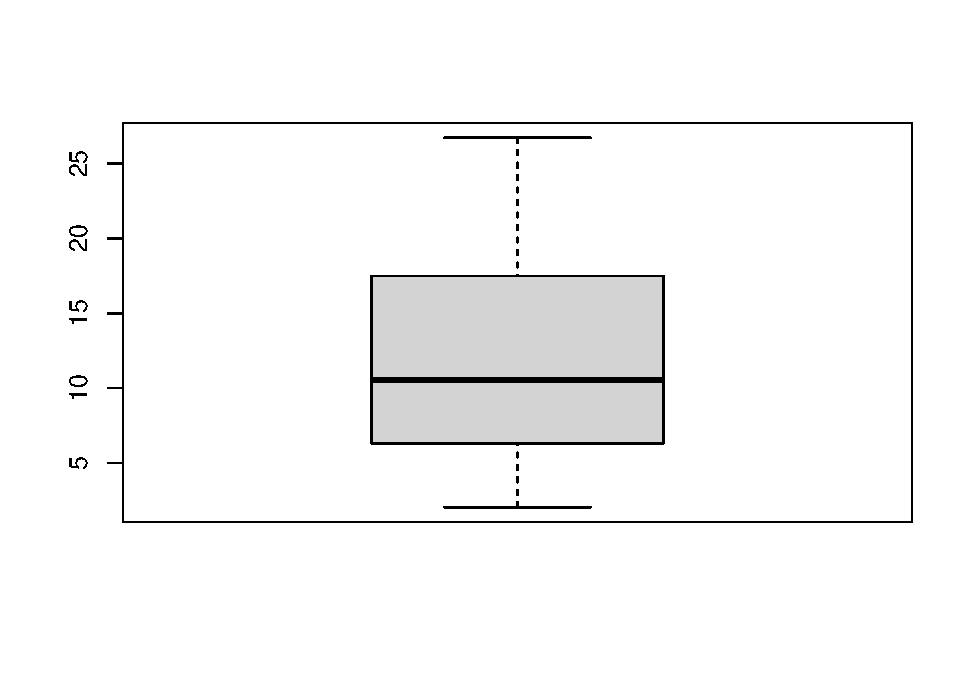
\includegraphics{_main_files/figure-latex/boxplot meals base-1.pdf}

With the basic boxplot we can quickly see that no outliers are present in our data and that our data is slight right skewed with the median is below the center of the boxplot. To label our boxplot, we can add the following arguments.

\begin{Shaded}
\begin{Highlighting}[]
\FunctionTok{boxplot}\NormalTok{(travel\_full\_clean\_subset}\SpecialCharTok{$}\NormalTok{Meal\_Inexpensive\_Restaurant,}
        \AttributeTok{main =} \StringTok{"Average price of resturant meals"}\NormalTok{, }\CommentTok{\# Title of the graph}
        \AttributeTok{xlab =} \StringTok{""}\NormalTok{, }\CommentTok{\# x{-}axis label}
        \AttributeTok{ylab=} \StringTok{"Dollar amount (CAD)"}\NormalTok{, }\CommentTok{\# y{-}axis label}
        \AttributeTok{col =} \StringTok{"white"}\NormalTok{) }\CommentTok{\# color of the boxplot}
\end{Highlighting}
\end{Shaded}

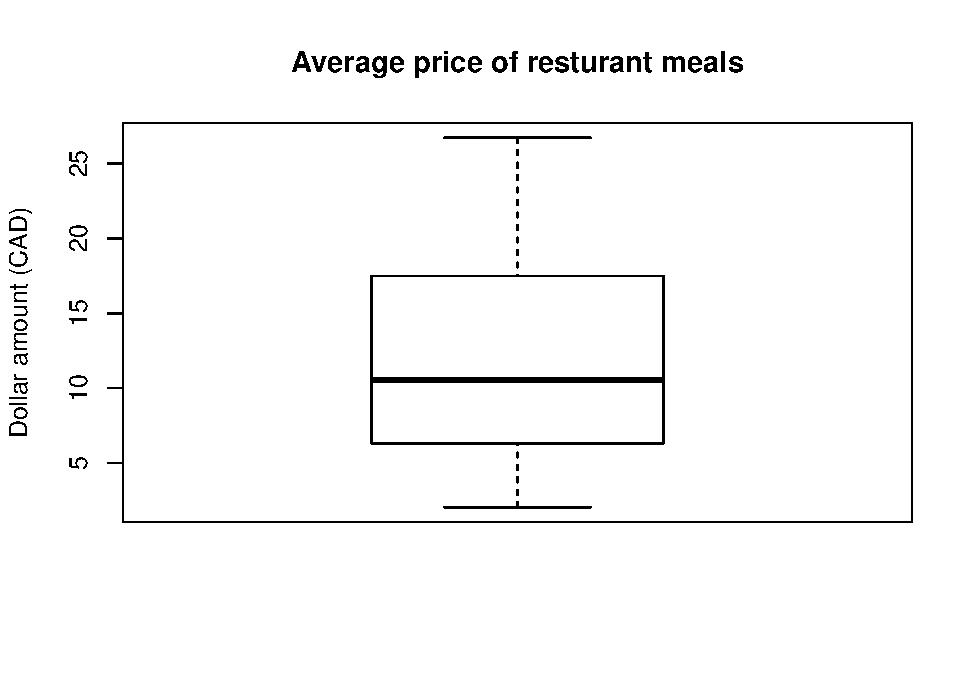
\includegraphics{_main_files/figure-latex/boxplot with labels base-1.pdf}

\hypertarget{histogram}{%
\subsection{Histogram}\label{histogram}}

Histograms can show the how our data is distributed. We can use the \textbf{hist( )} function to do this.

\begin{Shaded}
\begin{Highlighting}[]
\FunctionTok{hist}\NormalTok{(travel\_full\_clean\_subset}\SpecialCharTok{$}\NormalTok{Meal\_Inexpensive\_Restaurant, }
     \AttributeTok{breaks=} \DecValTok{30}\NormalTok{, }\CommentTok{\# number of breaks }
     \AttributeTok{ylim =} \FunctionTok{c}\NormalTok{(}\DecValTok{0}\NormalTok{,}\DecValTok{6}\NormalTok{),}
     \AttributeTok{main =} \StringTok{"Distribution of Average meal cost (CAD)"}\NormalTok{,}
     \AttributeTok{xlab =} \StringTok{""}\NormalTok{) }\CommentTok{\# y{-}axis limit}
\end{Highlighting}
\end{Shaded}

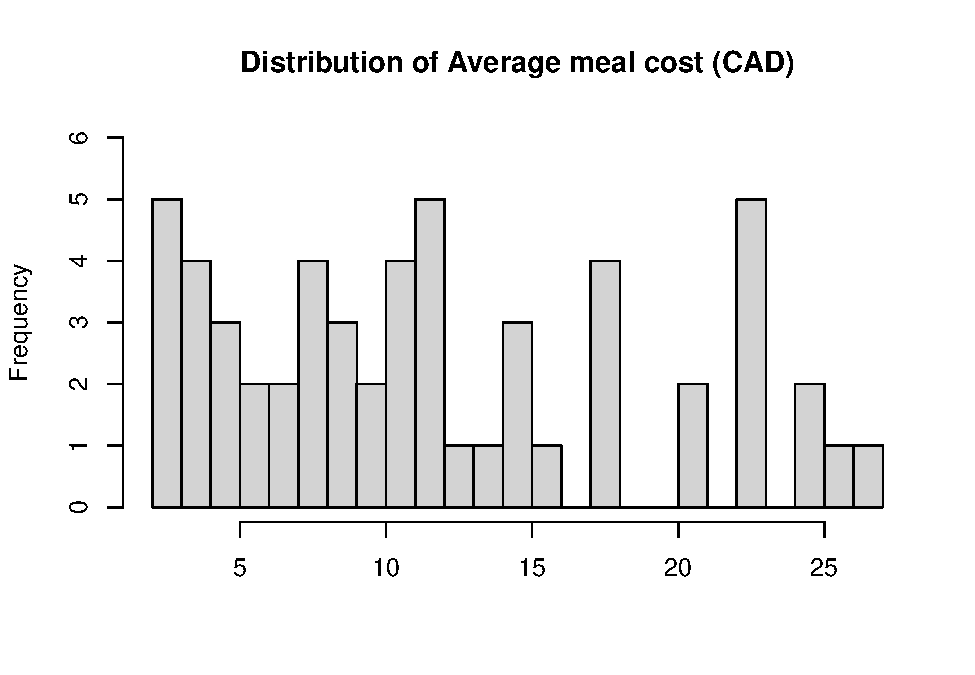
\includegraphics{_main_files/figure-latex/distribution of cost base-1.pdf}

\hypertarget{scatterplots}{%
\subsection{Scatterplots}\label{scatterplots}}

Scatterplots are useful to show a relationship between two different variables. For example, we can plot the the arrivals over time. Let's examine how Finland has changed over time. There are a few steps we need to take

\begin{itemize}
\item
  Filter our dataset to show data for Finland
\item
  Select the columns related to arrival (1995-2020)
\item
  Pivot our data from wide format to long format
\item
  Rename our columns to meaningful columns
\item
  Draw the scatterplot
\end{itemize}

\begin{Shaded}
\begin{Highlighting}[]
\FunctionTok{library}\NormalTok{(tidyr)}
\NormalTok{sweden\_travel }\OtherTok{\textless{}{-}}\NormalTok{ travel\_full\_clean\_subset }\SpecialCharTok{\%\textgreater{}\%}
  \FunctionTok{filter}\NormalTok{(country\_code}\SpecialCharTok{==}\StringTok{"SWE"}\NormalTok{ ) }\SpecialCharTok{\%\textgreater{}\%}
  \FunctionTok{select}\NormalTok{(}\FunctionTok{c}\NormalTok{(}\StringTok{"1995"}\SpecialCharTok{:}\StringTok{"2020"}\NormalTok{)) }\SpecialCharTok{\%\textgreater{}\%}
  \FunctionTok{gather}\NormalTok{() }\SpecialCharTok{\%\textgreater{}\%}
  \FunctionTok{rename}\NormalTok{(}\AttributeTok{years=}\NormalTok{ key,}
         \AttributeTok{arrivals=}\NormalTok{ value)}

\FunctionTok{plot}\NormalTok{(sweden\_travel}\SpecialCharTok{$}\NormalTok{years, sweden\_travel}\SpecialCharTok{$}\NormalTok{arrivals}\SpecialCharTok{/}\DecValTok{100000}\NormalTok{,}
     \AttributeTok{main=}\StringTok{"Number of Travellers from 1995 to 2020 (Sweden)"}\NormalTok{,}
     \AttributeTok{xlab=}\StringTok{"Years"}\NormalTok{,}
     \AttributeTok{ylab=}\StringTok{"Number of arrivals (x100,000)"}\NormalTok{) }
\end{Highlighting}
\end{Shaded}

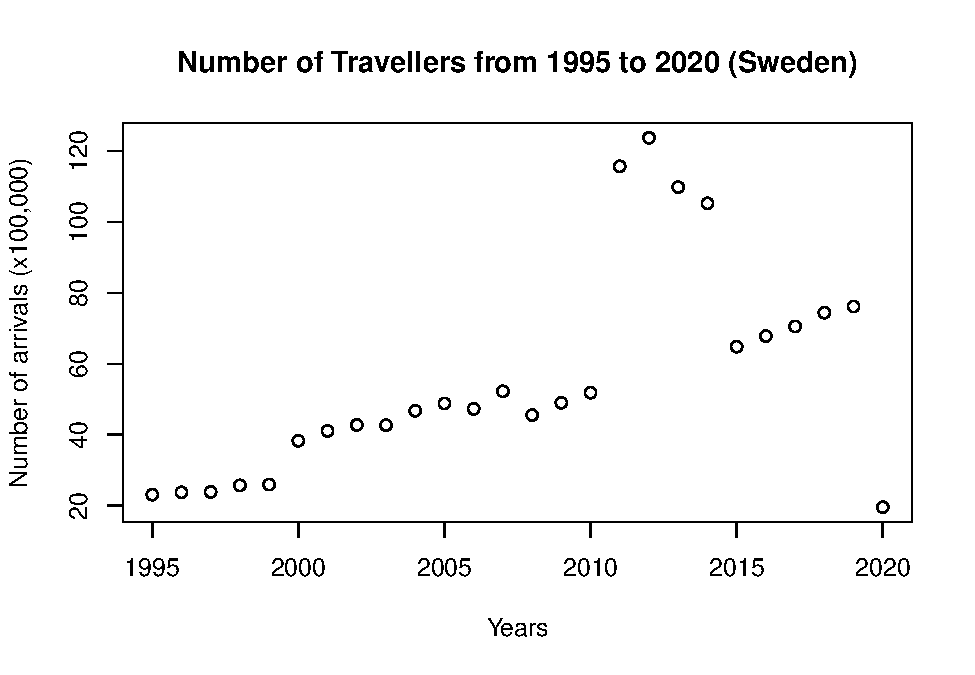
\includegraphics{_main_files/figure-latex/scatterplot base-1.pdf}

From the scatterplot, we see a steady increase in arrivals to sweeden over the years. We do see a few years between 2010, and 2015 with a high spike in arrivals which could indicate a few outliers in our data. To check we can run another boxplot on the arrivals data.

\begin{Shaded}
\begin{Highlighting}[]
\FunctionTok{boxplot}\NormalTok{(sweden\_travel}\SpecialCharTok{$}\NormalTok{arrivals}\SpecialCharTok{/}\DecValTok{100000}\NormalTok{,}
        \AttributeTok{main =} \StringTok{"Number of arrivals from 1995 {-} 2020 (Sweden)"}\NormalTok{, }\CommentTok{\# Title of the graph}
        \AttributeTok{xlab =} \StringTok{""}\NormalTok{, }\CommentTok{\# x{-}axis label}
        \AttributeTok{ylab=} \StringTok{"Number of arrivals (x100,000)"}\NormalTok{, }\CommentTok{\# y{-}axis label}
        \AttributeTok{col =} \StringTok{"white"}\NormalTok{) }\CommentTok{\# color of the boxplot)}
\end{Highlighting}
\end{Shaded}

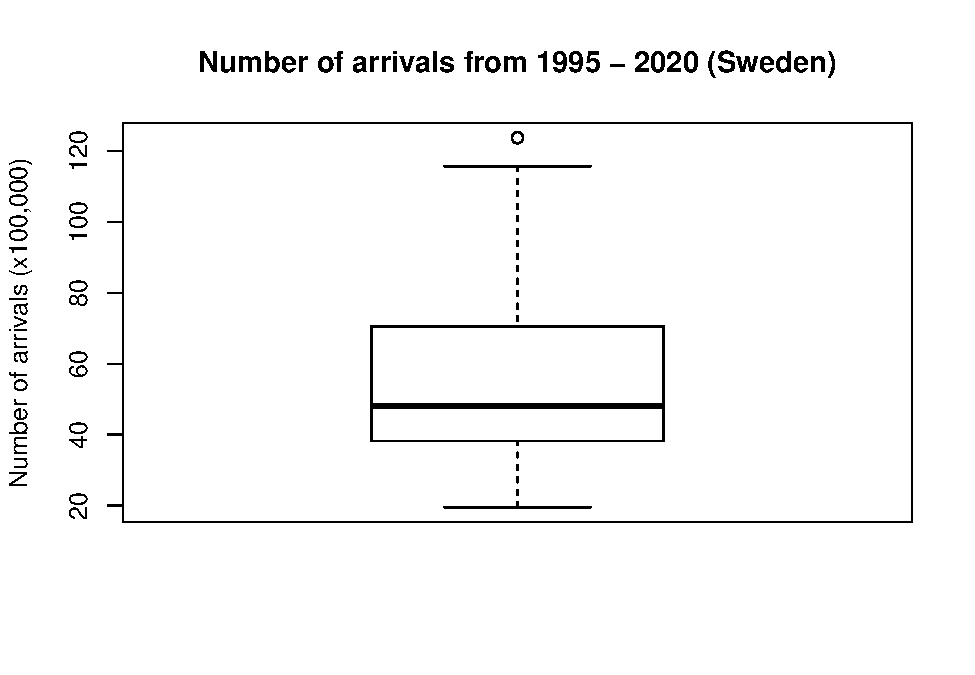
\includegraphics{_main_files/figure-latex/boxplot arrival base-1.pdf}

From the boxplot, we can see that there is at least 1 point that is an outlier in the data indicated by the circle above the maximum value

\hypertarget{ggplot2}{%
\section{ggplot2}\label{ggplot2}}

You can use the \textbf{ggplot2} package to create plots and figures instead of using the base R. It gives you more control over your plots to specify how you want it to look. Let's remake the previous 3 plots using \textbf{ggplot2}

Note

\begin{quote}
You can refer to the \textbf{ggplot2} \url{https://ggplot2.tidyverse.org/reference/index.html} to find all the possible plots that you can build with ggplot2
\end{quote}

First, we will need to install the package and then load the pack using the \textbf{library( )} function.

\begin{Shaded}
\begin{Highlighting}[]
\FunctionTok{library}\NormalTok{(ggplot2)}
\end{Highlighting}
\end{Shaded}

\hypertarget{boxplot}{%
\subsection{Boxplot}\label{boxplot}}

The basic structure for using \textbf{ggplot( )} is

\textbf{ggplot(data = x, aes(x = x-axis, y = y-axis)) + geom\_typeOfPlot() }

where \emph{aes} stands for aesthetic. This defines what variables you want to plot. For our boxplot, we want look at the meal prices as a whole so we only need to declare the y-variable.

\begin{Shaded}
\begin{Highlighting}[]
\FunctionTok{ggplot}\NormalTok{(}\AttributeTok{data =}\NormalTok{ travel\_full\_clean\_subset, }\FunctionTok{aes}\NormalTok{(}\AttributeTok{y=}\NormalTok{Meal\_Inexpensive\_Restaurant)) }\SpecialCharTok{+} 
  \FunctionTok{geom\_boxplot}\NormalTok{()}
\end{Highlighting}
\end{Shaded}

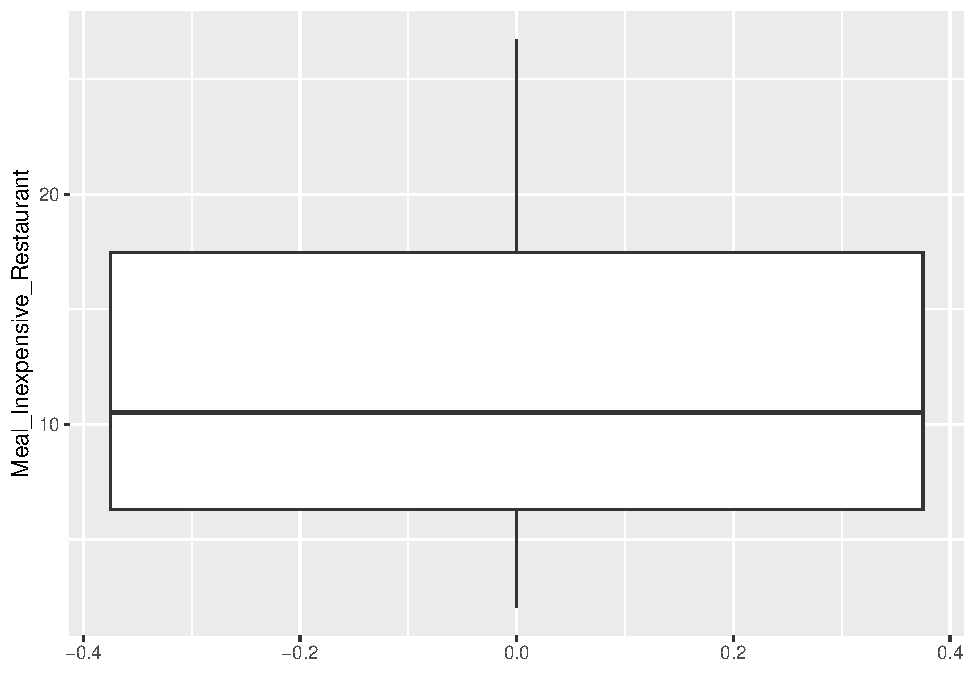
\includegraphics{_main_files/figure-latex/boxplot ggplot2-1.pdf}

We can also rename our axis in a simliar way to our base R plot by using the \textbf{labs( )} argument

\begin{Shaded}
\begin{Highlighting}[]
\FunctionTok{ggplot}\NormalTok{(}\AttributeTok{data =}\NormalTok{ travel\_full\_clean\_subset, }\FunctionTok{aes}\NormalTok{(}\AttributeTok{y=}\NormalTok{Meal\_Inexpensive\_Restaurant)) }\SpecialCharTok{+} 
  \FunctionTok{geom\_boxplot}\NormalTok{() }\SpecialCharTok{+}
  \FunctionTok{labs}\NormalTok{(}\AttributeTok{title=}\StringTok{"Average price of resturant meals"}\NormalTok{,}
       \AttributeTok{x=}\StringTok{""}\NormalTok{, }
       \AttributeTok{y =} \StringTok{"Dollar amount (CAD)"}\NormalTok{)}
\end{Highlighting}
\end{Shaded}

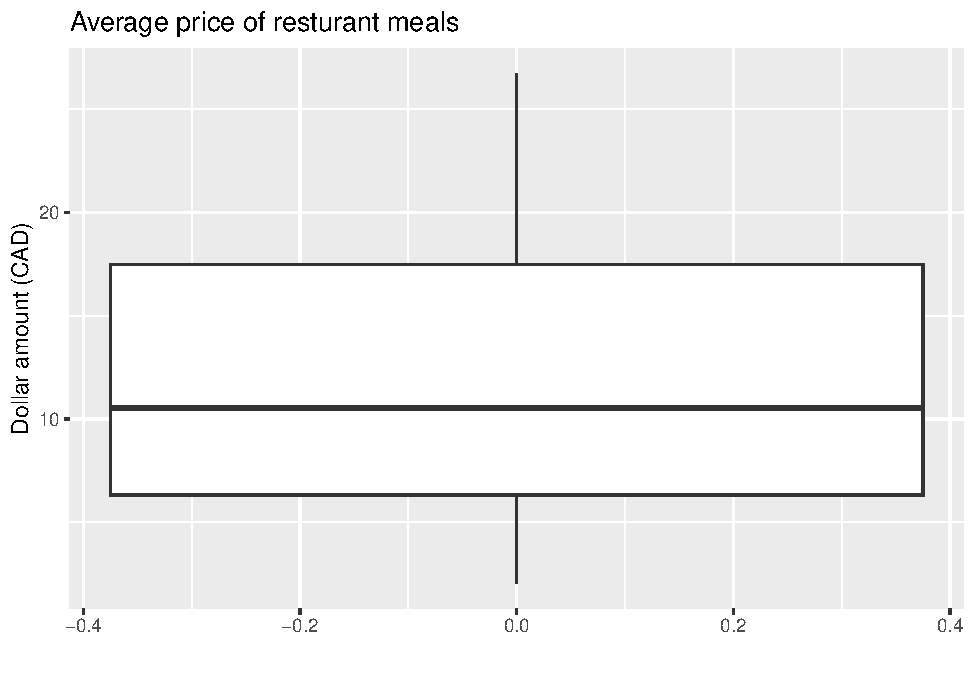
\includegraphics{_main_files/figure-latex/boxplot ggplot2 clean-1.pdf}

From here, we can customize the look of our boxplot with other arguments.

\hypertarget{histogram-1}{%
\subsection{Histogram}\label{histogram-1}}

We can do the same with our histogram. Instead of using \textbf{geom\_boxplot( )} we will use \textbf{geom\_histogram( )}

\begin{Shaded}
\begin{Highlighting}[]
\FunctionTok{ggplot}\NormalTok{(}\AttributeTok{data =}\NormalTok{ travel\_full\_clean\_subset, }\FunctionTok{aes}\NormalTok{(}\AttributeTok{x=}\NormalTok{Meal\_Inexpensive\_Restaurant)) }\SpecialCharTok{+} 
  \FunctionTok{geom\_histogram}\NormalTok{(}\AttributeTok{bins=}\DecValTok{30}\NormalTok{) }\SpecialCharTok{+}
  \FunctionTok{labs}\NormalTok{(}\AttributeTok{title=}\StringTok{"Distribution of Average meal cost (CAD)"}\NormalTok{,}
       \AttributeTok{y=} \StringTok{"Frequency"}\NormalTok{,}
       \AttributeTok{x=}\StringTok{""}\NormalTok{)}
\end{Highlighting}
\end{Shaded}

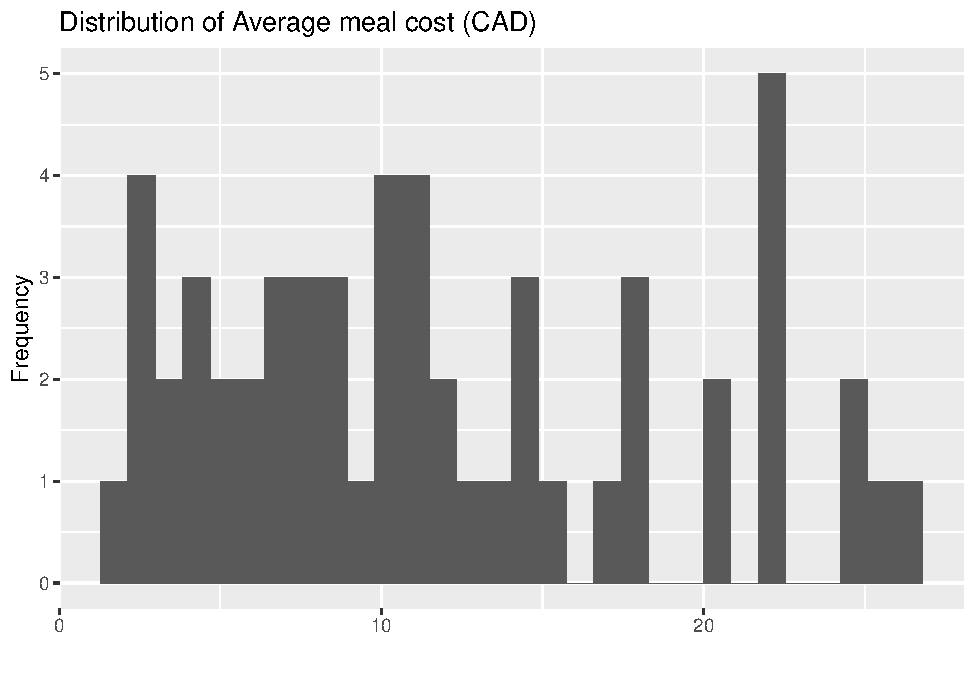
\includegraphics{_main_files/figure-latex/distribution of cost ggplot2-1.pdf}

\hypertarget{scatterplot}{%
\subsection{Scatterplot}\label{scatterplot}}

Similarly with the scatterplot, we can use \textbf{geom\_point( )}

\begin{Shaded}
\begin{Highlighting}[]
\FunctionTok{ggplot}\NormalTok{(}\AttributeTok{data =}\NormalTok{ sweden\_travel, }\FunctionTok{aes}\NormalTok{(}\AttributeTok{x=}\NormalTok{years, }\AttributeTok{y =}\NormalTok{ arrivals}\SpecialCharTok{/}\DecValTok{100000}\NormalTok{)) }\SpecialCharTok{+} 
  \FunctionTok{geom\_point}\NormalTok{() }\SpecialCharTok{+}
  \FunctionTok{labs}\NormalTok{(}\AttributeTok{title=}\StringTok{"Number of Travellers from 1995 to 2020 (Sweden)"}\NormalTok{,}
     \AttributeTok{x=}\StringTok{"Years"}\NormalTok{,}
     \AttributeTok{y=}\StringTok{"Number of arrivals (x100,000)"}\NormalTok{)}
\end{Highlighting}
\end{Shaded}

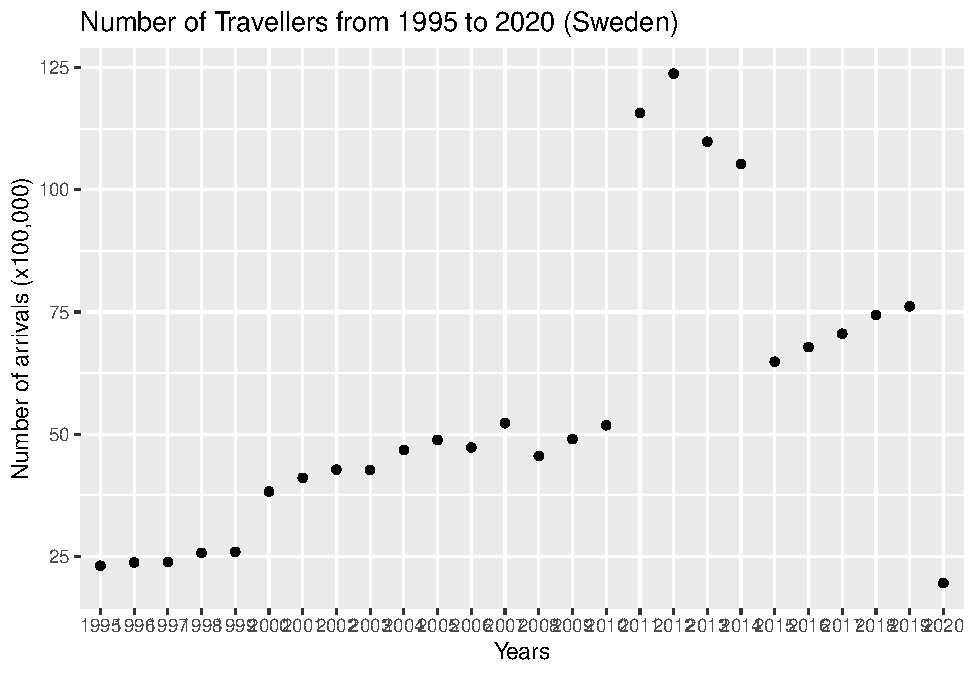
\includegraphics{_main_files/figure-latex/scatter ggplot2 base-1.pdf}

We can see that the scatterplot has the same trend but looks a little different. We can easily adjust the graph so it matches our previous one.

\begin{Shaded}
\begin{Highlighting}[]
\FunctionTok{ggplot}\NormalTok{(}\AttributeTok{data =}\NormalTok{ sweden\_travel, }\FunctionTok{aes}\NormalTok{(}\AttributeTok{x=}\NormalTok{years, }\AttributeTok{y =}\NormalTok{ arrivals}\SpecialCharTok{/}\DecValTok{100000}\NormalTok{)) }\SpecialCharTok{+} 
  \FunctionTok{geom\_point}\NormalTok{(}\AttributeTok{shape=}\DecValTok{1}\NormalTok{,}
             \AttributeTok{size=}\DecValTok{2}\NormalTok{) }\SpecialCharTok{+}
  \FunctionTok{labs}\NormalTok{(}\AttributeTok{title=}\StringTok{"Number of Travellers from 1995 to 2020 (Sweden)"}\NormalTok{,}
     \AttributeTok{x=}\StringTok{"Years"}\NormalTok{,}
     \AttributeTok{y=}\StringTok{"Number of arrivals (x100,000)"}\NormalTok{)}\SpecialCharTok{+}
  \FunctionTok{scale\_x\_discrete}\NormalTok{(}\AttributeTok{guide =} \FunctionTok{guide\_axis}\NormalTok{(}\AttributeTok{check.overlap =} \ConstantTok{TRUE}\NormalTok{)) }\SpecialCharTok{+}
  \FunctionTok{theme\_classic}\NormalTok{()}
\end{Highlighting}
\end{Shaded}

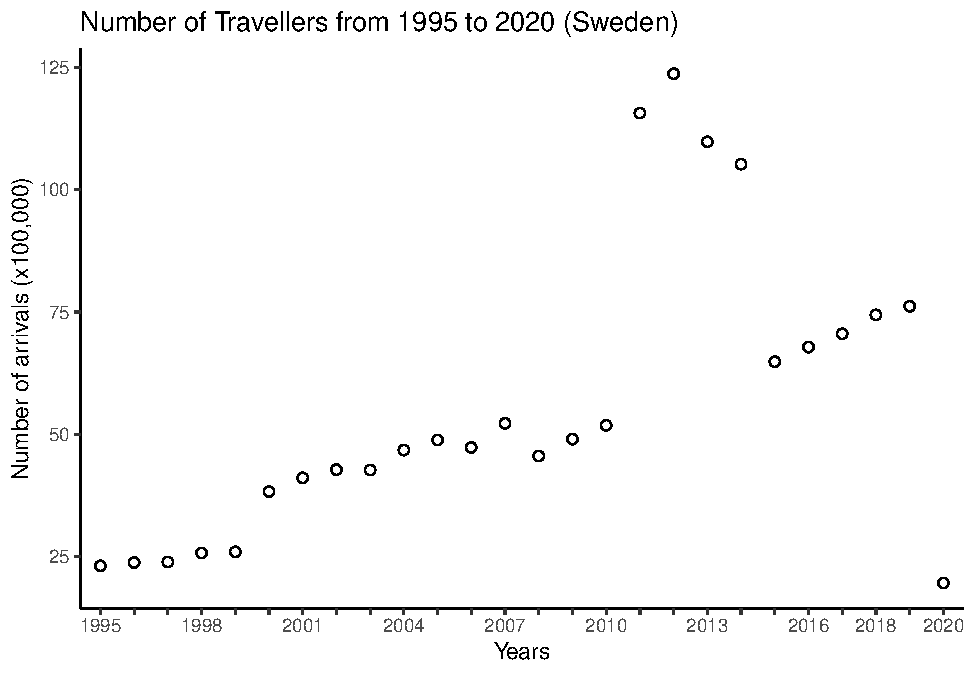
\includegraphics{_main_files/figure-latex/scatter ggplot2 clean-1.pdf}

By adding a few arguments we can create clean and meaningful graphs using \textbf{ggplot2}

\begin{Shaded}
\begin{Highlighting}[]
\FunctionTok{ggplot}\NormalTok{(}\AttributeTok{data =}\NormalTok{ sweden\_travel, }\FunctionTok{aes}\NormalTok{(}\AttributeTok{y=}\NormalTok{arrivals}\SpecialCharTok{/}\DecValTok{100000}\NormalTok{)) }\SpecialCharTok{+} 
  \FunctionTok{geom\_boxplot}\NormalTok{(}\AttributeTok{outlier.color =} \StringTok{"red"}\NormalTok{, }\AttributeTok{outlier.shape =} \DecValTok{1}\NormalTok{, }\AttributeTok{outlier.size =} \DecValTok{3}\NormalTok{) }\SpecialCharTok{+}
  \FunctionTok{labs}\NormalTok{(}\AttributeTok{title=}\StringTok{"Number of Travellers from 1995 to 2020 (Sweden)"}\NormalTok{,}
       \AttributeTok{x=}\StringTok{""}\NormalTok{, }
       \AttributeTok{y =} \StringTok{"Arrivals"}\NormalTok{)}
\end{Highlighting}
\end{Shaded}

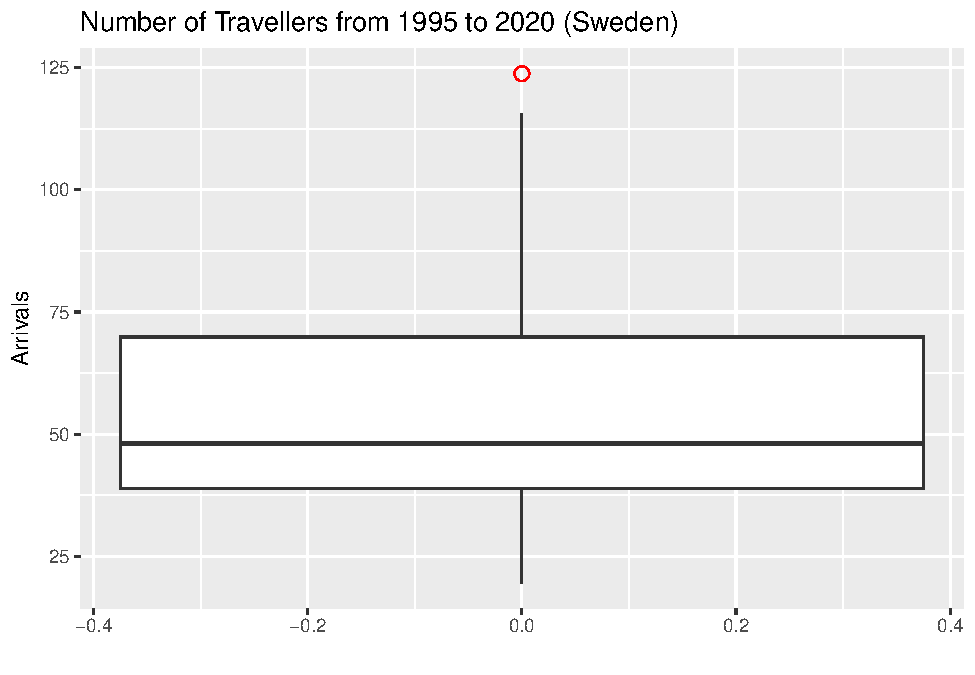
\includegraphics{_main_files/figure-latex/boxplot travel outlier ggplot2-1.pdf}

\hypertarget{exporting-plots}{%
\subsection{Exporting plots}\label{exporting-plots}}

Once you are finished with creating your desired graph, you can export the file as a pdf or other vector image formats for journals. Let's use our last boxplot on the number of arrivals as a example. First we need to save the boxplot as a variable.

\begin{Shaded}
\begin{Highlighting}[]
\NormalTok{boxplot\_arrivals\_swe }\OtherTok{\textless{}{-}} \FunctionTok{ggplot}\NormalTok{(}\AttributeTok{data =}\NormalTok{ sweden\_travel, }\FunctionTok{aes}\NormalTok{(}\AttributeTok{y=}\NormalTok{arrivals}\SpecialCharTok{/}\DecValTok{100000}\NormalTok{)) }\SpecialCharTok{+} 
  \FunctionTok{geom\_boxplot}\NormalTok{(}\AttributeTok{outlier.color =} \StringTok{"red"}\NormalTok{, }\AttributeTok{outlier.shape =} \DecValTok{1}\NormalTok{, }\AttributeTok{outlier.size =} \DecValTok{3}\NormalTok{) }\SpecialCharTok{+}
  \FunctionTok{labs}\NormalTok{(}\AttributeTok{title=}\StringTok{"Number of Travellers from 1995 to 2020 (Sweden)"}\NormalTok{,}
       \AttributeTok{x=}\StringTok{""}\NormalTok{, }
       \AttributeTok{y =} \StringTok{"Arrivals"}\NormalTok{)}
\end{Highlighting}
\end{Shaded}

Next, we will use the \textbf{ggsave( )} function and specify the location, the format, and the height and width we want to save the image as.

\begin{Shaded}
\begin{Highlighting}[]
\FunctionTok{ggsave}\NormalTok{(}\StringTok{"/Users/markly/boxplot\_swe\_arrival.pdf"}\NormalTok{, }\AttributeTok{plot =}\NormalTok{ boxplot\_arrivals\_swe, }\AttributeTok{device =} \StringTok{"pdf"}\NormalTok{, }\AttributeTok{width =} \DecValTok{12}\NormalTok{, }\AttributeTok{height =} \DecValTok{6}\NormalTok{, }\AttributeTok{dpi=}\DecValTok{150}\NormalTok{)}
\end{Highlighting}
\end{Shaded}

Note:

\begin{quote}
We can save images in different formats including
\end{quote}

\begin{itemize}
\tightlist
\item
  png, eps, ps, tex, jpeg, tiff, bmp, svg or wmf
\end{itemize}

\hypertarget{gtsummary}{%
\section{gtsummary}\label{gtsummary}}

Another powerful package that helps with data visulizuation is \textbf{gtsummary} which can quickly generate summary tables. We will need to install the package and load the package using the \textbf{library( )} function.

\begin{Shaded}
\begin{Highlighting}[]
\FunctionTok{library}\NormalTok{(gtsummary)}
\end{Highlighting}
\end{Shaded}

Let's say we are interested in summarizing the meal and ticket costs in a table. First, we will need to subset that from our dataset and then pass that into the \textbf{tbl\_summary()} function.

\begin{Shaded}
\begin{Highlighting}[]
\NormalTok{travel\_full\_clean\_subset }\SpecialCharTok{\%\textgreater{}\%}
  \FunctionTok{select}\NormalTok{(}\FunctionTok{c}\NormalTok{(Meal\_Inexpensive\_Restaurant,one\_way\_ticket\_local)) }\SpecialCharTok{\%\textgreater{}\%}
  \FunctionTok{tbl\_summary}\NormalTok{()}
\end{Highlighting}
\end{Shaded}

\begin{verbatim}
## Table printed with `knitr::kable()`, not {gt}. Learn why at
## https://www.danieldsjoberg.com/gtsummary/articles/rmarkdown.html
## To suppress this message, include `message = FALSE` in code chunk header.
\end{verbatim}

\begin{tabular}{l|c}
\hline
**Characteristic** & **N = 55**\\
\hline
Meal\_Inexpensive\_Restaurant & 11 (6, 17)\\
\hline
one\_way\_ticket\_local & 1.20 (0.50, 2.20)\\
\hline
\end{tabular}

This produced a summary table of all the meals and ticket information giving us the \textbf{median} and \textbf{IQR} without any additional steps. We can customize this table a bit further by adding a few arguments.

\begin{Shaded}
\begin{Highlighting}[]
\NormalTok{travel\_full\_clean\_subset }\SpecialCharTok{\%\textgreater{}\%}
  \FunctionTok{select}\NormalTok{(}\FunctionTok{c}\NormalTok{(Meal\_Inexpensive\_Restaurant,one\_way\_ticket\_local)) }\SpecialCharTok{\%\textgreater{}\%}
  \FunctionTok{tbl\_summary}\NormalTok{(}\AttributeTok{label =} \FunctionTok{list}\NormalTok{(}\StringTok{"Meal\_Inexpensive\_Restaurant"}\SpecialCharTok{\textasciitilde{}}\StringTok{"Meal Price"}\NormalTok{,}
                           \StringTok{"one\_way\_ticket\_local"}\SpecialCharTok{\textasciitilde{}}\StringTok{"One{-}way Ticket Price"}\NormalTok{)) }\SpecialCharTok{\%\textgreater{}\%}
  \FunctionTok{modify\_header}\NormalTok{(}\AttributeTok{label =} \StringTok{"**Variable**"}\NormalTok{) }\SpecialCharTok{\%\textgreater{}\%} \CommentTok{\# update the column header}
  \FunctionTok{bold\_labels}\NormalTok{() }
\end{Highlighting}
\end{Shaded}

\begin{verbatim}
## Table printed with `knitr::kable()`, not {gt}. Learn why at
## https://www.danieldsjoberg.com/gtsummary/articles/rmarkdown.html
## To suppress this message, include `message = FALSE` in code chunk header.
\end{verbatim}

\begin{tabular}{l|c}
\hline
**Variable** & **N = 55**\\
\hline
\_\_Meal Price\_\_ & 11 (6, 17)\\
\hline
\_\_One-way Ticket Price\_\_ & 1.20 (0.50, 2.20)\\
\hline
\end{tabular}

\textbf{gtsummary} is also great for separating and summarizing groups in the same table. We can add region information to our data set using a left join. After saving our new dataframe, we can select only the variables needed, region, meal price, and ticket price, and apply the \textbf{gtsummary( )} function to output a table based on region.

\begin{Shaded}
\begin{Highlighting}[]
\NormalTok{region}\OtherTok{\textless{}{-}} \FunctionTok{read.csv}\NormalTok{(}\StringTok{"data/csv\_region.csv"}\NormalTok{)}
\NormalTok{region\_select }\OtherTok{\textless{}{-}}\NormalTok{region }\SpecialCharTok{\%\textgreater{}\%}
  \FunctionTok{select}\NormalTok{(}\FunctionTok{c}\NormalTok{(alpha}\FloatTok{.3}\NormalTok{,region)) }\SpecialCharTok{\%\textgreater{}\%}
  \FunctionTok{rename}\NormalTok{(}\AttributeTok{country\_code =}\NormalTok{ alpha}\FloatTok{.3}\NormalTok{)}

\NormalTok{travel\_region }\OtherTok{\textless{}{-}}\NormalTok{ travel\_full\_clean\_subset }\SpecialCharTok{\%\textgreater{}\%}
  \FunctionTok{select}\NormalTok{(}\FunctionTok{c}\NormalTok{(}\DecValTok{1}\SpecialCharTok{:}\DecValTok{4}\NormalTok{)) }\SpecialCharTok{\%\textgreater{}\%}
  \FunctionTok{inner\_join}\NormalTok{(.,region\_select,}\AttributeTok{by=}\StringTok{"country\_code"}\NormalTok{)}

\NormalTok{travel\_region }\SpecialCharTok{\%\textgreater{}\%} 
  \FunctionTok{select}\NormalTok{(}\SpecialCharTok{{-}}\FunctionTok{c}\NormalTok{(Country,country\_code))}\SpecialCharTok{\%\textgreater{}\%}
  \FunctionTok{tbl\_summary}\NormalTok{(}\AttributeTok{by=}\NormalTok{region,}
              \AttributeTok{label =} \FunctionTok{list}\NormalTok{(}\StringTok{"Meal\_Inexpensive\_Restaurant"}\SpecialCharTok{\textasciitilde{}}\StringTok{"Meal Price"}\NormalTok{,}
                           \StringTok{"one\_way\_ticket\_local"}\SpecialCharTok{\textasciitilde{}}\StringTok{"One{-}way Ticket Price"}\NormalTok{)) }\SpecialCharTok{\%\textgreater{}\%}
  \FunctionTok{modify\_header}\NormalTok{(}\AttributeTok{label =} \StringTok{"**Variable**"}\NormalTok{) }\SpecialCharTok{\%\textgreater{}\%} \CommentTok{\# update the column header}
  \FunctionTok{bold\_labels}\NormalTok{()}
\end{Highlighting}
\end{Shaded}

\begin{verbatim}
## Table printed with `knitr::kable()`, not {gt}. Learn why at
## https://www.danieldsjoberg.com/gtsummary/articles/rmarkdown.html
## To suppress this message, include `message = FALSE` in code chunk header.
\end{verbatim}

\begin{tabular}{l|c|c|c|c|c}
\hline
**Variable** & **Africa**, N = 6 & **Americas**, N = 10 & **Asia**, N = 14 & **Europe**, N = 23 & **Oceania**, N = 2\\
\hline
\_\_Meal Price\_\_ & 5 (4, 8) & 10 (6, 12) & 6 (3, 10) & 16 (12, 22) & 22 (21, 22)\\
\hline
\_\_One-way Ticket Price\_\_ & 0.49 (0.33, 1.01) & 0.85 (0.76, 1.29) & 0.49 (0.35, 0.93) & 2.20 (1.29, 4.20) & 3.46 (3.18, 3.75)\\
\hline
\end{tabular}

\begin{Shaded}
\begin{Highlighting}[]
\NormalTok{travel\_full\_clean\_subset }\SpecialCharTok{\%\textgreater{}\%}
  \FunctionTok{inner\_join}\NormalTok{(.,region\_select,}\AttributeTok{by=}\StringTok{"country\_code"}\NormalTok{) }\SpecialCharTok{\%\textgreater{}\%}
  \FunctionTok{select}\NormalTok{(}\FunctionTok{c}\NormalTok{(Meal\_Inexpensive\_Restaurant,one\_way\_ticket\_local,}\StringTok{"2015"}\SpecialCharTok{:}\StringTok{"2020"}\NormalTok{,region)) }\SpecialCharTok{\%\textgreater{}\%}
  \FunctionTok{tbl\_summary}\NormalTok{(}\AttributeTok{by=}\NormalTok{region)}
\end{Highlighting}
\end{Shaded}

\begin{verbatim}
## Table printed with `knitr::kable()`, not {gt}. Learn why at
## https://www.danieldsjoberg.com/gtsummary/articles/rmarkdown.html
## To suppress this message, include `message = FALSE` in code chunk header.
\end{verbatim}

\begin{tabular}{l|c|c|c|c|c}
\hline
**Characteristic** & **Africa**, N = 6 & **Americas**, N = 10 & **Asia**, N = 14 & **Europe**, N = 23 & **Oceania**, N = 2\\
\hline
Meal\_Inexpensive\_Restaurant & 5 (4, 8) & 10 (6, 12) & 6 (3, 10) & 16 (12, 22) & 22 (21, 22)\\
\hline
one\_way\_ticket\_local & 0.49 (0.33, 1.01) & 0.85 (0.76, 1.29) & 0.49 (0.35, 0.93) & 2.20 (1.29, 4.20) & 3.46 (3.18, 3.75)\\
\hline
2015 & 3,534,500 (1,308,000, 9,246,250) & 3,531,500 (2,639,500, 5,859,500) & 6,151,000 (2,706,750, 14,025,375) & 9,317,000 (3,576,500, 30,849,000) & 5,289,000 (4,209,000, 6,369,000)\\
\hline
2016 & 3,881,500 (1,490,000, 9,438,750) & 3,756,000 (2,585,250, 6,327,500) & 6,511,000 (2,745,750, 15,182,000) & 10,223,000 (4,066,500, 31,838,000) & 5,881,500 (4,687,750, 7,075,250)\\
\hline
2017 & 4,751,500 (1,641,000, 10,418,000) & 4,166,000 (2,695,500, 6,703,750) & 7,014,000 (3,164,000, 16,578,750) & 10,926,000 (4,554,500, 33,456,000) & 6,269,000 (4,996,000, 7,542,000)\\
\hline
2018 & 5,478,000 (1,737,500, 11,441,500) & 4,289,500 (2,693,500, 6,762,500) & 7,855,500 (3,368,000, 17,833,500) & 11,720,000 (5,056,500, 34,848,500) & 6,552,000 (5,205,000, 7,899,000)\\
\hline
2019 & 5,900,000 (1,656,250, 12,189,000) & 4,382,000 (2,761,500, 6,895,250) & 8,413,000 (3,717,750, 18,839,250) & 12,552,000 (5,290,500, 35,723,500) & 6,677,000 (5,282,500, 8,071,500)\\
\hline
2020 & 1,301,500 (536,250, 2,604,500) & 1,362,850 (771,875, 3,598,500) & 1,837,000 (907,000, 3,999,000) & 3,382,000 (1,306,500, 11,775,000) & 1,412,000 (1,204,000, 1,620,000)\\
\hline
\end{tabular}

With both \textbf{ggplot2} and \textbf{gtsummary}, we have lots of tools to use to display and communicate our data.

\hypertarget{regression}{%
\chapter{Regression}\label{regression}}

R is a statistical computing language which is capable of performing multiple statistical models including

\begin{itemize}
\item
  lm(y \textasciitilde{} x) linear regression model with one explanatory variable
\item
  lm(y \textasciitilde{} x1 + x2 + x3) multiple regression, a linear model with multiple explanatory variables
\item
  glm(y \textasciitilde{} x, family = poisson) generalized linear model, poisson distribution; see ?family to see those supported, including binomial, gaussian, poisson, etc.
\item
  glm(y \textasciitilde{} x + y, family = binomial) glm for logistic regression
\item
  aov(y \textasciitilde{} x) analysis of variance (same as lm except in the summary)
\item
  gam(y \textasciitilde{} x) generalized additive models
\item
  tree(y \textasciitilde{} x) or rpart(y \textasciitilde{} x) regression/classification trees
\end{itemize}

\hypertarget{linear-regression}{%
\section{Linear regression}\label{linear-regression}}

Linear regression is a statistical method used for predictive analysis where we want to show if there is a linear relationship between an \textbf{independent predictor} variable and a \textbf{dependent output} variable. The goal is to build a mathematical formula that defines y as a function of the x variable. Once, we built a statistically significant model, it's possible to use it for predicting future outcome on the basis of new x values.

From the previous scatterplot, we noticed that there might be a relationship between the years and arrivals for Sweden. We can try to perform a linear regression to determine if that is the case. The hypothesis we want to propose is that the number of arrivals to Sweden increases linearly per year.

The general formula for a linear model is

\[Y_{i} = \beta_{0} + \beta_{1}X_{1} + \epsilon \]
where

\[Y_{i} = \text{Dependent Variable}\]
\[\beta_{0} = \text{Constant/Intercept}\]
\[\beta_{1} = \text{Slope/Intercept}\]
\[X_{1} = \text{Independent Variable}\]
\[\epsilon = \text{Error Term}\]

For our model, we would write out our linear regression equation as

\[\text{arrivals} = \beta_{0} + \beta_{1}*\text{Years} + \epsilon\]

\hypertarget{assumptions-of-linear-regression}{%
\subsection{Assumptions of Linear Regression}\label{assumptions-of-linear-regression}}

Before we begin with linear regression, there are some assumptions that need to be satisfied. We can use the \texttt{LINE} acronym to explain these assumptions.

\begin{itemize}
\item
  \textbf{L}inearity of residuals - There needs to be a linear relationship between the dependent and independent variables(s)
\item
  \textbf{I}ndependance of residuals - The error terms should not be dependent on one another. For example, in time series, the next value is dependent on the previous one.
\item
  \textbf{N}ormal distribution of residuals - The mean residuals should follow a normal distribution with a mean equal to zero or close to zero.
\item
  \textbf{E}qual variance of the residuals - The error terms must have constant variance
\end{itemize}

\hypertarget{residuals}{%
\subsection{Residuals}\label{residuals}}

Residuals represent the difference between the predicted value and the observed value. The formula for residuals is.

\[\text{Residual} - \text{actual y value} - \text{predicted y value}\]
This is what residuals look like on a linear regression plot.

\begin{figure}
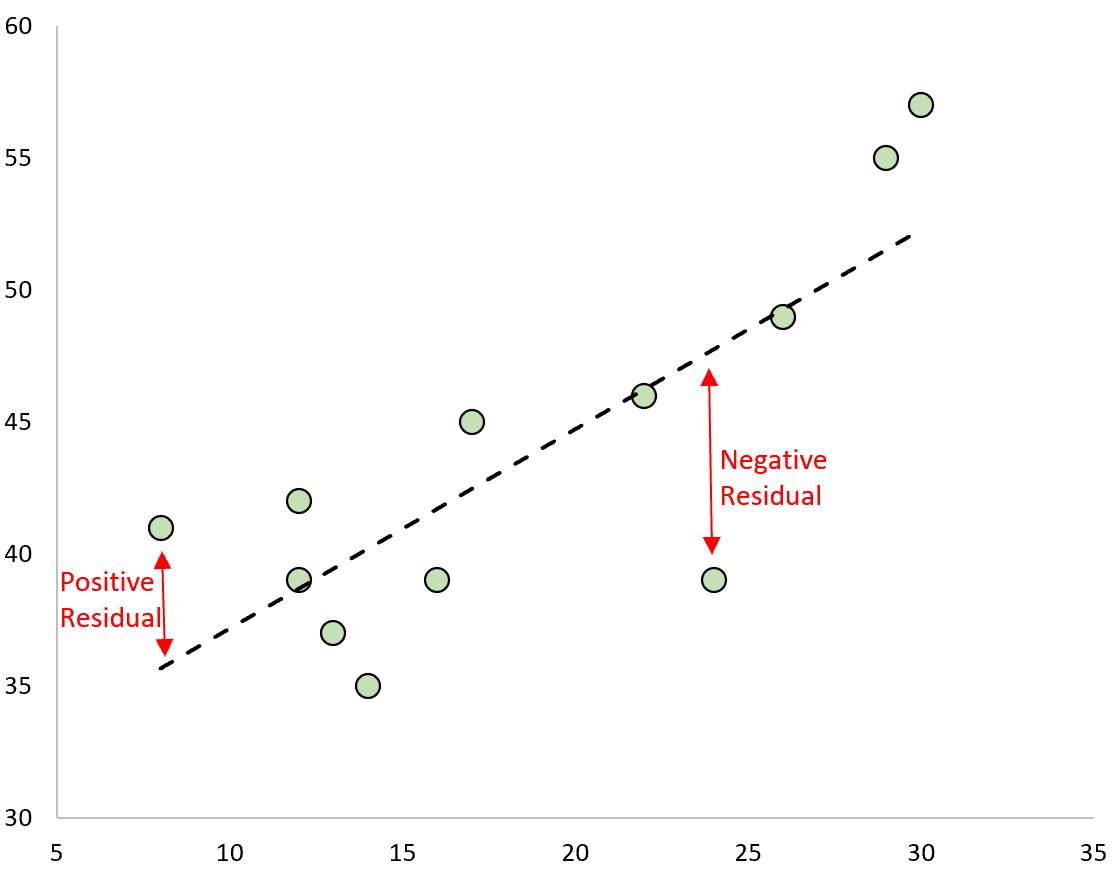
\includegraphics[width=15.5in]{images/residuals2} \caption{Residuals on a linear regression}\label{fig:unnamed-chunk-22}
\end{figure}

\hypertarget{creating-our-intial-model}{%
\subsection{Creating our intial model}\label{creating-our-intial-model}}

To create a linear model, we use this function when we have one explanatory variable

\begin{quote}
\textbf{lm({[}target{]} \textasciitilde{} {[}predictor / features{]}, data = {[}data source{]})}
\end{quote}

In this case our y-variable is the number of \texttt{arrivals} and the x-variable is the \texttt{years}

Note:

\begin{quote}
The years variable in our dataframe is a \emph{character}. We need to convert it to a numeric to perform the linear regression.
\end{quote}

\begin{Shaded}
\begin{Highlighting}[]
\NormalTok{swe\_model }\OtherTok{\textless{}{-}} \FunctionTok{lm}\NormalTok{(arrivals}\SpecialCharTok{\textasciitilde{}}\FunctionTok{as.numeric}\NormalTok{(sweden\_travel}\SpecialCharTok{$}\NormalTok{years),}\AttributeTok{data=}\NormalTok{sweden\_travel)}
\NormalTok{swe\_model}
\end{Highlighting}
\end{Shaded}

\begin{verbatim}
## 
## Call:
## lm(formula = arrivals ~ as.numeric(sweden_travel$years), data = sweden_travel)
## 
## Coefficients:
##                     (Intercept)  as.numeric(sweden_travel$years)  
##                      -470402333                           237113
\end{verbatim}

\hypertarget{interpretation-of-results}{%
\subsection{Interpretation of results}\label{interpretation-of-results}}

We can print out a summary of our model using the \textbf{summary( )} function. This will give us information on the intercept, standard error, p-value, test-statistic, \(r^2\) value.

\begin{Shaded}
\begin{Highlighting}[]
\FunctionTok{summary}\NormalTok{(swe\_model)}
\end{Highlighting}
\end{Shaded}

\begin{verbatim}
## 
## Call:
## lm(formula = arrivals ~ as.numeric(sweden_travel$years), data = sweden_travel)
## 
## Residuals:
##      Min       1Q   Median       3Q      Max 
## -6608564  -826391  -507921   -40090  5703338 
## 
## Coefficients:
##                                   Estimate Std. Error t value Pr(>|t|)    
## (Intercept)                     -470402333  126815668  -3.709  0.00109 ** 
## as.numeric(sweden_travel$years)     237113      63170   3.754  0.00098 ***
## ---
## Signif. codes:  0 '***' 0.001 '**' 0.01 '*' 0.05 '.' 0.1 ' ' 1
## 
## Residual standard error: 2416000 on 24 degrees of freedom
## Multiple R-squared:  0.3699, Adjusted R-squared:  0.3436 
## F-statistic: 14.09 on 1 and 24 DF,  p-value: 0.0009798
\end{verbatim}

In this output, the estimate column shows the estimates of our beta coefficients \(\beta_0\) and \(\beta_1\).
The intercept (\(\beta_0\)) is -470,402,333 and the coefficient of years variable is 237,113. We can rewrite our original equation with our new results

\[\text{arrivals} = \beta_{0} + \beta_{1}*\text{Years} + \epsilon\]
\[\text{arrivals} = -470,402,333 + 237,113*\text{Years} + \epsilon\]
In writen form, we would say

\begin{itemize}
\item
  If the Years is equal to zero, we can expect -470,402,333 arrivals
\item
  For every 1 increase in Years, we can expect 237,113 arrivals
\end{itemize}

The first point doesn't make any sense since we can't have year equal to 0.

\hypertarget{assumption-checking}{%
\subsection{Assumption checking}\label{assumption-checking}}

If we plot our linear regression, it will give us diagnostic plots that will help determine if our linear model satisfies certain assumptions

\begin{itemize}
\item
  \textbf{Residual vs Fitted} - Used to check linear relationship assumptions.
\item
  \textbf{Normal Q-Q}- Used to check if the residuals are normally distributed.
\item
  \textbf{Scale-Location} - Used to check homogeneity of variance.
\item
  \textbf{Residuals vs Leverage} - Used to check for influential cases or extreme values that might influence the regression results.
\end{itemize}

\begin{Shaded}
\begin{Highlighting}[]
\FunctionTok{plot}\NormalTok{(swe\_model,}\AttributeTok{which=}\NormalTok{(}\DecValTok{1}\NormalTok{))}
\end{Highlighting}
\end{Shaded}

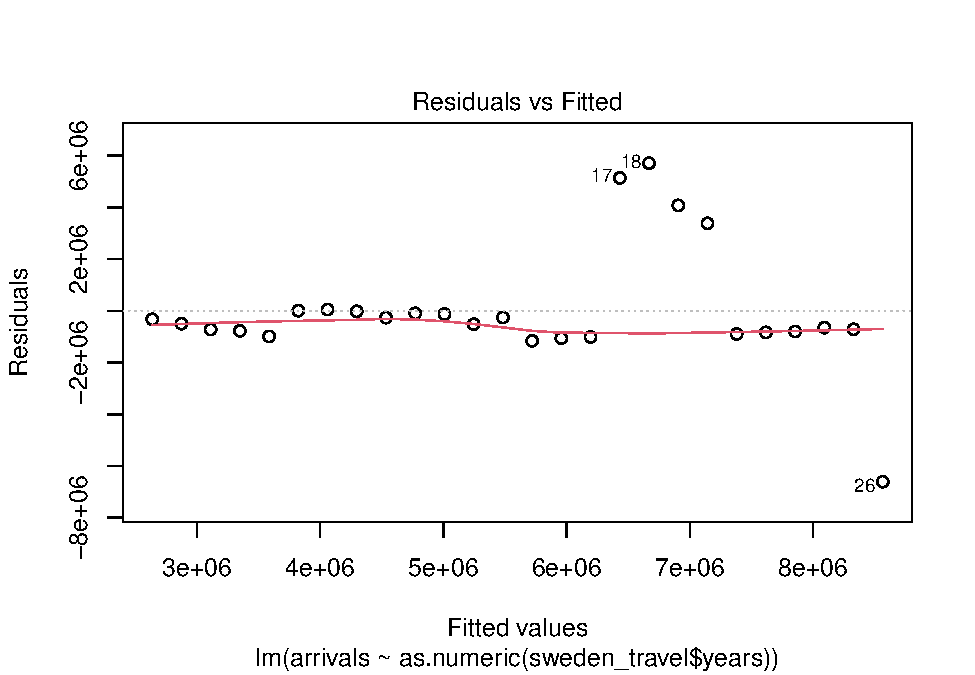
\includegraphics{_main_files/figure-latex/lm resdiual vs fitted plots-1.pdf}

If our linearity assumption is met, we should see no pattern and the red line show be fairly flat. In our model, we see that this is the case with a few points cluster of points that lie above the line.

\begin{Shaded}
\begin{Highlighting}[]
\FunctionTok{plot}\NormalTok{(swe\_model,}\AttributeTok{which=}\NormalTok{(}\DecValTok{2}\NormalTok{))}
\end{Highlighting}
\end{Shaded}

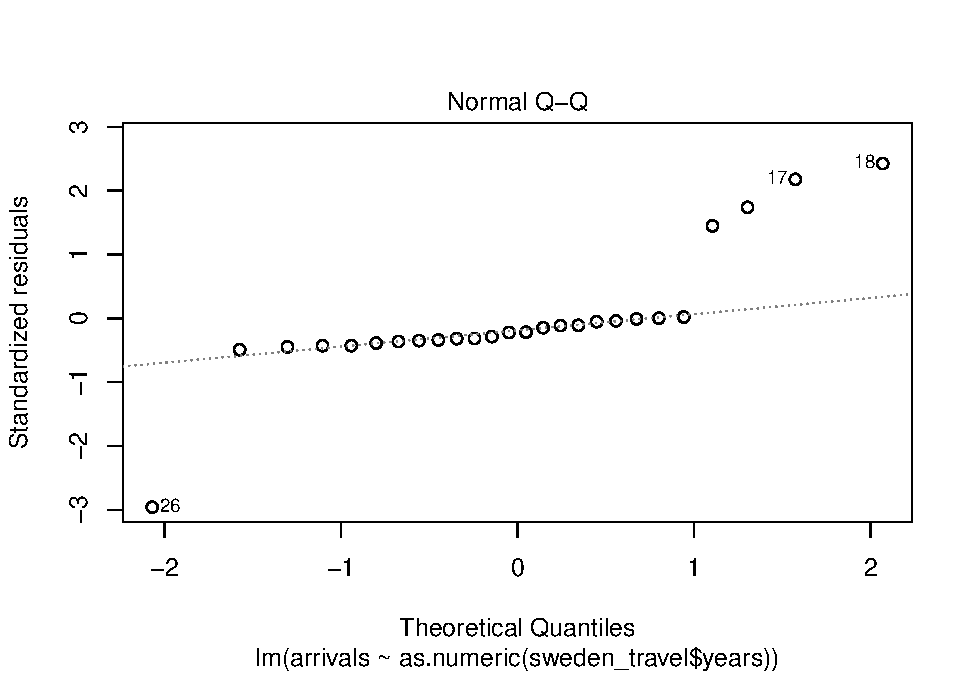
\includegraphics{_main_files/figure-latex/lm normal q-q plots-1.pdf}

For our normality assumption we can use the second plot, the Normal Q-Q plot. what we expect to see is a 45 degree line and most of the points should lie on this line. For our model this does not seem to hold true as our points are closer to a 10-20 degree slope.

\begin{Shaded}
\begin{Highlighting}[]
\FunctionTok{plot}\NormalTok{(swe\_model,}\AttributeTok{which=}\NormalTok{(}\DecValTok{3}\NormalTok{))}
\end{Highlighting}
\end{Shaded}

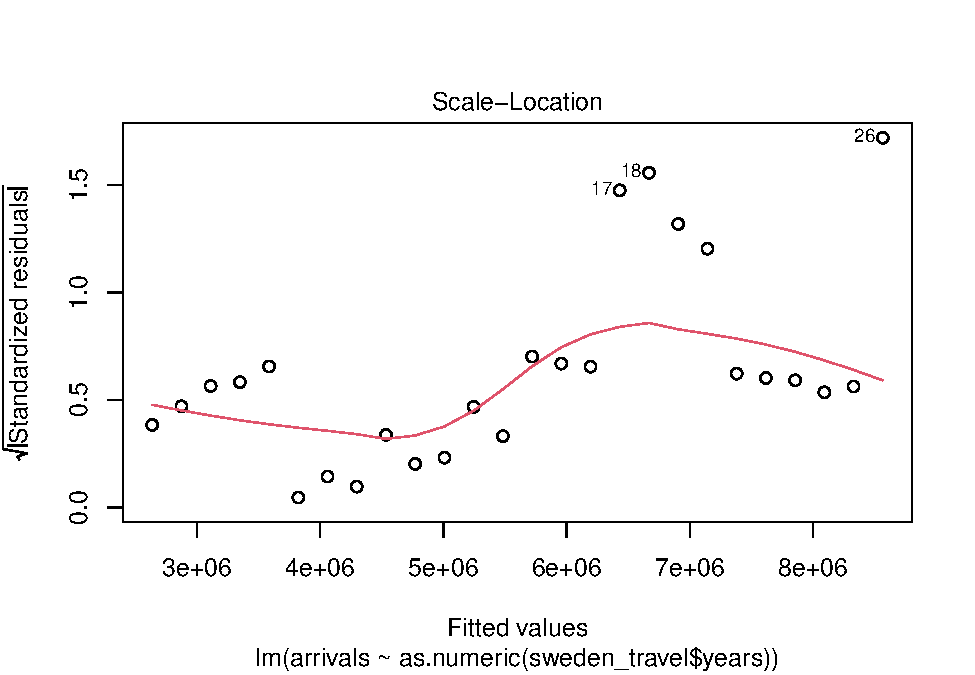
\includegraphics{_main_files/figure-latex/lm scale-location plots-1.pdf}

To check our assumption of constant variance we can use the third plot, the scale-location plot. What we want to see here are points scattered randomly and the red line to be close to horizontal. However, what we see is there is a pattern and that indicates that the constant variance assumption does not hold true for this model. What we can try to do is transform our y variable using:

\begin{itemize}
\item
  Log transformation
\item
  Square Root transformation
\item
  Cube Root transformation
\end{itemize}

\begin{Shaded}
\begin{Highlighting}[]
\FunctionTok{par}\NormalTok{(}\AttributeTok{mfrow=}\FunctionTok{c}\NormalTok{(}\DecValTok{1}\NormalTok{,}\DecValTok{2}\NormalTok{))}
\FunctionTok{plot}\NormalTok{(swe\_model, }\AttributeTok{which=}\FunctionTok{c}\NormalTok{(}\DecValTok{4}\NormalTok{,}\DecValTok{5}\NormalTok{))}
\end{Highlighting}
\end{Shaded}

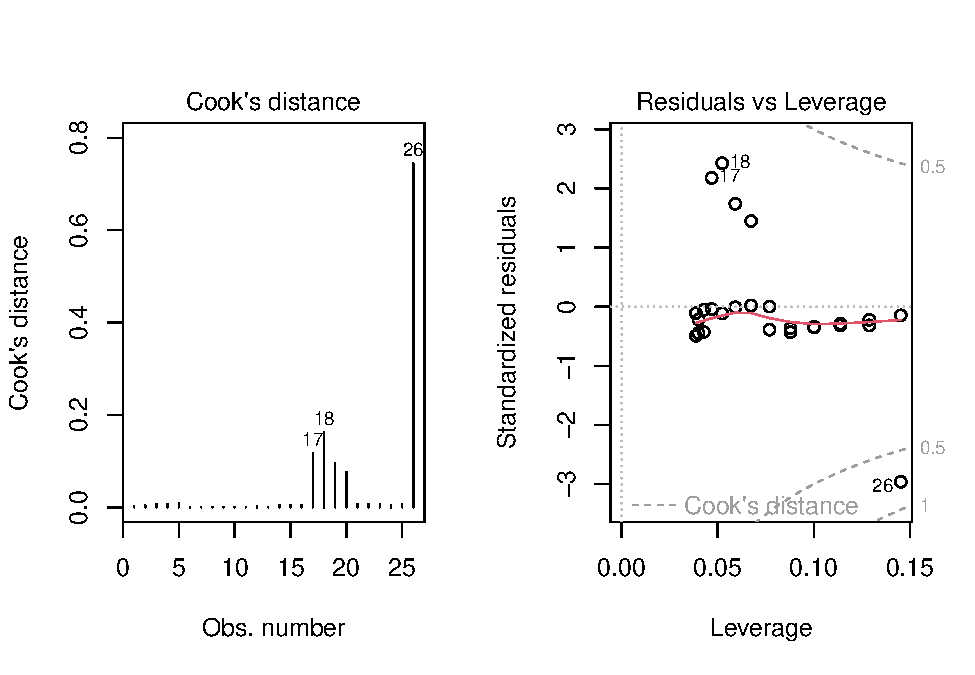
\includegraphics{_main_files/figure-latex/lm leverage-1.pdf}

The last plot is the Residuals vs leverage plot. Leverage refers to to the extent where our coefficients would change if we removed an observation from the data set. Points that have high leverage would noticeably change our coefficients. If a point falls outside of the red dashed line, cook's distance, it is considered to be a influential point and requires further investigation. For our model, we don't have any points that are influential.

\hypertarget{summary}{%
\subsection{Summary}\label{summary}}

Our initial hypothesis was

\begin{quote}
Does the number of arrivals increase linearly over time (Years)?
\end{quote}

Since this model does not satisfy the normality assumption and the constant variance assumption that is required for linear regression, we cannot say that the number of arrivals increases linearly as years increases.

\hypertarget{next-steps}{%
\subsection{Next steps}\label{next-steps}}

Since our linear regression model did not work, we can try using a different model that might be better in explaining trend. In this case, our independent variable is the number of arrivals which count data. Count data is data that does not contain any non-negative integer numbers, (0,1,2,3\ldots). The usual function to deal with count data is a \texttt{Poisson\ Regression}, which is a generalized linear model used when the independent variable deals with count data that follows a Poisson distribution. It assumes the logarithm of expected values (mean) that can be modeled into a linear form by some unknown parameters.

\hypertarget{other-capabilties}{%
\chapter{Other capabilties}\label{other-capabilties}}

We can create and perform other tasks using R. We will go quickly go through some R's capabilities and things you can do with R including

\begin{itemize}
\item
  R-bookdown
\item
  R-Shiny
\item
  R-Markdown
\item
  Machine learning
\end{itemize}

\hypertarget{r-bookdown}{%
\section{R-bookdown}\label{r-bookdown}}

With R you can create books using the \textbf{R-bookdown} package. This entire workshop was created using R-bookdown. With R-Bookdown, we can create books and long form articles and reports. We can output these books as a PDF, LaTeX, HTML, EPUB and word files. It is a great way to produce a structured document with chaptures, sections, subsections and appendices.

You can visit \url{https://bookdown.org/} to find out more about bookdown.

\hypertarget{r-shiny}{%
\section{R-Shiny}\label{r-shiny}}

We can build web applications and dashboards using \textbf{R-Shiny}. This is an alternative way to present data in a more interactive way. Some examples of R-Shiny applications can be found on \url{https://shiny.rstudio.com/gallery/} which includes COVID-19 trackers, A/B Testing sample size calculators, Nutritional calculators, Hospital dashboards and genome browsers.

\hypertarget{r-markdown}{%
\section{R-markdown}\label{r-markdown}}

One advantage to using R-studio is the ability to output reports into as a word, html, or pdf format. Using the \textbf{knit} function capabilities, we can create reports that can be easily reproduced since the code and outputs are all in the same R-markdown file. This is an advantage if you need to generate reports if data gets updated.

\hypertarget{machine-learning}{%
\section{Machine learning}\label{machine-learning}}

We can perform machine learning tasks in R using the \textbf{caret} and \textbf{factoextra} packages. This includes models like

\begin{itemize}
\item
  Random forests
\item
  Decisions Trees
\item
  XGBoost
\item
  K-means
\item
  Neural Networks
\end{itemize}

It is important to note that although these technologies can be powerful and provide a new insight to existing data, we have to ask ourselves if it is necessary and why we would want to attempt to use machine learning.

  \bibliography{book.bib,packages.bib}

\end{document}
